%                      Code_Saturne version 1.3
%                      ------------------------
%
%     This file is part of the Code_Saturne Kernel, element of the
%     Code_Saturne CFD tool.
% 
%     Copyright (C) 1998-2007 EDF S.A., France
%
%     contact: saturne-support@edf.fr
% 
%     The Code_Saturne Kernel is free software; you can redistribute it
%     and/or modify it under the terms of the GNU General Public License
%     as published by the Free Software Foundation; either version 2 of
%     the License, or (at your option) any later version.
% 
%     The Code_Saturne Kernel is distributed in the hope that it will be
%     useful, but WITHOUT ANY WARRANTY; without even the implied warranty
%     of MERCHANTABILITY or FITNESS FOR A PARTICULAR PURPOSE.  See the
%     GNU General Public License for more details.
% 
%     You should have received a copy of the GNU General Public License
%     along with the Code_Saturne Kernel; if not, write to the
%     Free Software Foundation, Inc.,
%     51 Franklin St, Fifth Floor,
%     Boston, MA  02110-1301  USA
%
%-----------------------------------------------------------------------
%
%%%%%%%%%%%%%%%%%%%%%%%%%%%%%%%%%%%%%%%%%%%%%%%%%%%%%%%%%%%%%%%%%%%%%%
%                                                                    %
%                                                                    %
%                                                                    %
% Titre :           Code_Saturne user manual                         %
%                                                                    %
%                                                                    %
%                                                                    %
%%%%%%%%%%%%%%%%%%%%%%%%%%%%%%%%%%%%%%%%%%%%%%%%%%%%%%%%%%%%%%%%%%%%%%
\documentclass[a4paper,10pt,twoside]{article}

%
%%%%%%%%%%%%%%%%%%%%%%%%%%%%%%%%%%%%%%%%%%%%%%%%%%%%%%%%%%%%%%%%%%%%%%
% PACKAGES OBLIGATOIRES
\usepackage{../../style/csdoc}
%
%%%%%%%%%%%%%%%%%%%%%%%%%%%%%%%%%%%%%%%%%%%%%%%%%%%%%%%%%%%%%%%%%%%%%%

%
%%%%%%%%%%%%%%%%%%%%%%%%%%%%%%%%%%%%%%%%%%%%%%%%%%%%%%%%%%%%%%%%%%%%%%
% PACKAGES ET COMMANDES POUR LE DOCUMENTS PDF ET LES HYPERLIENS
\usepackage[pdftex,
            bookmarksopen=true,
            colorlinks=true,
            linkcolor=blue,
            filecolor=blue,
            urlcolor=blue,
            citecolor=blue]{hyperref}
\hypersetup{%
  pdftitle = {Code_Saturne version 1.3 practical user's guide},
  pdfauthor = {MFEE},
  pdfpagemode = UseOutlines
}
\pdfinfo{/CreationDate (D:20030429000000-01 00 )}
%
% Pour avoir les Thumbnails a l'ouverture du document sous ACROREAD :
% pdfpagemode = UseThumbs
%
%%%%%%%%%%%%%%%%%%%%%%%%%%%%%%%%%%%%%%%%%%%%%%%%%%%%%%%%%%%%%%%%%%%%%%
% R�ALISATION D'UN INDEX
\usepackage{makeidx}
\makeindex
%
%%%%%%%%%%%%%%%%%%%%%%%%%%%%%%%%%%%%%%%%%%%%%%%%%%%%%%%%%%%%%%%%%%%%%%
% PACKAGES ALLTT D'ENVIRONNEMENT VERBATIM AMELIORE
\usepackage{alltt}
%
%%%%%%%%%%%%%%%%%%%%%%%%%%%%%%%%%%%%%%%%%%%%%%%%%%%%%%%%%%%%%%%%%%%%%%
% MACROS SUPPLEMENTAIRES
% \newcommand{/...}{...}
%
% repertoire et extension des images
\newcommand{\repgraphics}{../graphics}
\newcommand{\extgraphics}{pdf}
%
\newbox\tempbox
\newcommand{\motcle}[7]{%
   \noindent
   \setbox\tempbox\hbox{\hspace*{2.5cm}}
   \makebox[2.5cm][l]{#1}\index{#1}\makebox[1.3cm][l]{#2}\makebox[6.cm][l]{#3}%
   \makebox[4.cm][l]{[#4]}#5\hspace{1cm}#6\\
   \hangindent\wd\tempbox\quad\ignorespaces#7\bigskip}
\newcommand{\motcleb}[7]{%
   \noindent
   \setbox\tempbox\hbox{\hspace*{2.5cm}}
   \makebox[2.5cm][l]{\bf #1}\index{#1}\makebox[1.3cm][l]{#2}\makebox[6.cm][l]{#3}%
   \makebox[4.cm][l]{[#4]}#5\hspace{1cm}#6\\
   \hangindent\wd\tempbox\quad\ignorespaces#7\bigskip}
%
%\newcommand{\variab}[4]{%
%       \hangindent\wd\tempbox\noindent{#2\index{#1} [#3] \quad\\}
%       \hspace*{0.5cm}\ignorespaces#4.}
\newcommand{\variab}[4]{%
       \setbox\tempbox\hbox{IFACEL [E] : }
       \hangindent\wd\tempbox\noindent{#2\index{#1} [#3] :\quad}\ignorespaces#4.}
\newcommand{\variablist}[4]{%
       \setbox\tempbox\hbox{IFACEL [E] : }
       \hangindent\wd\tempbox\noindent{#2\index{#1} [#3] :\quad}\ignorespaces#4\quad}
%\newcommand{\variab}[4]{%
%       \setbox\tempbox\hbox{#2 [#3] :\quad}
%       \hangindent\wd\tempbox\noindent{#2\index{#1} [#3] :\quad}\ignorespaces#4.}
%
%%%%%%%%%%%%%%%%%%%%%%%%%%%%%%%%%%%%%%%%%%%%%%%%%%%%%%%%%%%%%%%%%%%%%%
% INFO POUR PAGES DE GARDES
\titreCS{\CS\ version~\verscs\ practical user's guide}
\docassociesCS{}
\resumeCS{This document presents all the necessary elements to run a calculation
with \CS\ version \verscs. It then lists all the variables of the code
which may be useful for more advanced utilisation.
The user subroutines of all the modules within the code are also documented.
Eventually, for each key word and user-modifiable parameter in the code,
their definition, allowed values, default values and conditions for use are given.
These key words and parameters are grouped under headings
based on their function. An alphabetical index list is also given at the end of
the document for easier consultation.}
%
%%%%%%%%%%%%%%%%%%%%%%%%%%%%%%%%%%%%%%%%%%%%%%%%%%%%%%%%%%%%%%%%%%%%%%
% DEBUT DU DOCUMENT
\begin{document}
\pdfgraphics
\def\contentsname{\textbf{\normalsize TABLE OF CONTENTS}\pdfbookmark[1]{Table of
contents}{contents}}
\def\indexname{Index of the main variables and keywords}

\pdfbookmark[1]{Flyleaf}{pdg}
\large
\makepdgCS
\normalsize

\input summary

\passepage

\begin{center}\begin{singlespace}
\tableofcontents
\end{singlespace}\end{center}
%
%%%%%%%%%%%%%%%%%%%%%%%%%%%%%%%%%%%%%%%%%%%%%%%%%%%%%%%%%%%%%%%%%%%%%%
% CORPS DU DOCUMENT
%
\passepage
%-------------------------------------------------------------------------------

% This file is part of code_saturne, a general-purpose CFD tool.
%
% Copyright (C) 1998-2022 EDF S.A.
%
% This program is free software; you can redistribute it and/or modify it under
% the terms of the GNU General Public License as published by the Free Software
% Foundation; either version 2 of the License, or (at your option) any later
% version.
%
% This program is distributed in the hope that it will be useful, but WITHOUT
% ANY WARRANTY; without even the implied warranty of MERCHANTABILITY or FITNESS
% FOR A PARTICULAR PURPOSE.  See the GNU General Public License for more
% details.
%
% You should have received a copy of the GNU General Public License along with
% this program; if not, write to the Free Software Foundation, Inc., 51 Franklin
% Street, Fifth Floor, Boston, MA 02110-1301, USA.

%-------------------------------------------------------------------------------

\nopagebreak
%==================================
%==================================
\section{Introduction}
%==================================
%==================================

This document is a practical user guide for \CS version \verscs.
It is the result of the joint effort of
all the members in the development team.

This document provides practical information for the usage of \CS.
For more details about the algorithms and their numerical implementation,
please refer to the reports
 \cite{ijvf}, and \cite{mechitoua98},
and to the theoretical documentation \cite{theory}.

The latest updated version of this document is available on-line with the version of \CS
and accessible through the command
\texttt{code\_saturne info --guide theory}.

This document presents some the necessary elements to run a calculation
with \CS version \verscs. It then lists all the variables of the code
which may be useful for more advanced users.
The user functions of all the modules within the code are then documented.
Eventually, for each keyword and user-modifiable parameter in the code,
their definition, allowed values, default values and conditions for use are given.
These keywords and parameters are grouped under headings
based on their function. An alphabetical index is also given at the end of
the document for easier reference.

In addition to the present user guide, a complete
\texttt{Doxygen} documentation is available with \CS. It can provide
information about the implementation such as details on variables used
throughout the solver and the user functions. It also provides an easily
explorable set of user function examples and Fortran-C naming references for
quantities linked to the mesh or the physical fields.

The user documentation is in the process of migration from this pdf documentation
to the Doxygen documentation, so the user should first lok there.
One can access the \texttt{Doxygen} main page through \doxygenfile{index.html}{this link} or from a terminal by typing the following command:
\texttt{code\_saturne info --guide theory}.

%==================================
\section{Basic modelling setup}
%==================================

%==================================
\subsection{Manage boundary conditions}
%==================================

\texttt{cs\_user\_boundary\_conditions} is the second compulsory function for every calculation launched
without interface (except in the case of specific physics where the
corresponding boundary condition user function must be used).

When using the interface, only complex boundary conditions (input profiles, conditions varying in time, ...)
need to be defined with \texttt{cs\_user\_boundary\_conditions}.
In the case of a calculation launched without the
interface, all the boundary conditions must appear in \texttt{cs\_user\_boundary\_conditions}.

\texttt{cs\_user\_boundary\_conditions} is essentially constituted of loops on boundary
face subsets. Users can uses a function \texttt{cs\_boundary\_zone\_by\_name("criterion")}
allow selecting the boundary faces with respect to their group(s), their
color(s) or geometric criteria. If needed, geometric and
physical variables are also available to the user. These allow him
to select the boundary faces using other criteria.

For more details about the treatment of boundary conditions, the user
may refer to the theoretical and computer documentation \cite{theory} of
the function \texttt{condli} (for wall conditions, see
\texttt{clptur}) (to access this document on a workstation, use
\mbox{\texttt{code\_saturne~info --guide theory}}).

From the user point of view, the boundary conditions are fully
defined by three arrays\footnote{Except with Lagrangian boundary condition}:
\texttt{bc\_type[n\_b\_faces]}\index{\texttt{bc\_type}},
\texttt{icodcl[n\_b\_faces*nvar]}\index{\texttt{icodcl}} and
\texttt{rcodcl[n\_b\_faces*nvar*3]}\index{\texttt{rcodcl}}.
\begin{list}{-}{}
\item \texttt{bc\_type[face\_id]} defines the type of the face \texttt{face\_id}
      (input, wall, ...).
\item \texttt{icodcl[ivar*n\_b\_faces + face\_id]} defines the type of boundary
      condition for the variable \texttt{ivar = cs\_field\_get\_key\_int(field, keyvar) - 1 and keyvar = cs\_field\_key\_id("variable\_id")} on the face \texttt{face\_id}
      (Dirichlet, flux ...).
\item \texttt{rcodcl[ivar*n\_b\_faces + face\_id]} gives the numerical values associated with the
      boundary condition (value of the Dirichlet condition, of the flux ...).
\end{list}

In Fortran, the matching array dimensions are:

\texttt{itypfb(nfabor)}\index{\texttt{itypfb}},
\texttt{icodcl(nfabor,nvar)}\index{\texttt{icodcl}} and
\texttt{rcodcl(nfabor,nvar,3)}\index{\texttt{rcodcl}}.
\begin{list}{-}{}
\item \texttt{itypfb(ifac)} defines the type of the face \texttt{ifac}.
\item \texttt{icodcl(ifac,ivar)} defines the type of boundary
      condition for the variable \texttt{ivar} on the face \texttt{ifac}.
\item \texttt{rcodcl(ifac,ivar,.)} gives the numerical values associated with the
      boundary condition.
\end{list}

In the case of standard boundary conditions (see
\S\ref{sec:prg_clstandard}), it is sufficient to complete \texttt{bc\_type[face\_id]} and
parts of the array \texttt{rcodcl}; the array \texttt{icodcl} and most of \texttt{rcodcl} are filled automatically. For non-standard boundary
conditions (see \S\ref{sec:prg_clnonstandard}), the arrays \texttt{icodcl} and
\texttt{rcodcl} must be fully completed.

%==================================
\subsubsection{Coding of standard boundary conditions}
%==================================
\label{sec:prg_clstandard}%
The standard keywords used by the indicator \texttt{bc\_type} are, in C:
\texttt{CS\_INLET}\index{CS\_INLET}, \texttt{CS\_SMOOTHWALL\index{CS\_SMOOTHWALL}},
\texttt{CS\_ROUGHWALL\index{CS\_ROUGHWALL}}, \texttt{CS\_SYMMETRY\index{CS\_SYMMETRY}},
\texttt{CS\_OUTLET\index{CS\_OUTLET}}, \texttt{CS\_FREE\_INLET\index{CS\_FREE\_INLET}}, \texttt{CS\_FREE\_SURFACE\index{CS\_FREE\_SURFACE}},
\texttt{CS\_CONVECTIVE\_INLET\index{CS\_CONVECTIVE\_INLET}} and \texttt{CS\_INDEF\index{CS\_INDEF}}.

With the matching Fortran names:
\texttt{ientre\index{ientre}}, \texttt{iparoi\index{iparoi}},
\texttt{iparug\index{iparug}}, \texttt{isymet\index{isymet}},
\texttt{isolib\index{isolib}}, \texttt{ifrent\index{ifrent}}, \texttt{ifresf\index{ifresf}},
\texttt{i\_convective\_inlet\index{i\_convective\_inlet}} and \texttt{iindef\index{iindef}}.

\begin{list}{$\bullet$}{}
\item If \texttt{bc\_type[face\_id] = CS\_INLET}: inlet face.

\begin{list}{$\rightarrow$}{}
\item Zero-flux condition for pressure and Dirichlet condition for all
      other variables. The value of the Dirichlet condition must be given in
      \texttt{rcodcl[ivar*n\_b\_faces + face\_id]} for every value of \texttt{ivar}, except for
      \texttt{ivar=cs\_field\_get\_key\_int(CS\_F\_(p), cs\_field\_key\_id("variable\_id")) - 1}. The other values of \texttt{rcodcl} and
      \texttt{icodcl} are filled automatically.
\end{list}

\item If \texttt{bc\_type[face\_id]=CS\_SMOOTHWALL}: smooth solid wall face, impermeable and with friction.

\begin{list}{$\rightarrow$}{}
\item the eventual sliding wall velocity of the face is
      found in \texttt{rcodcl[(ivar+ii)*n\_b\_faces + face\_id]} (\texttt{ivar=cs\_field\_get\_key\_int(CS\_F\_(vel),
      cs\_field\_key\_id("variable\_id")-1)} and ii being
      \texttt{0}, \texttt{1} or \texttt{2}). The initial
      values of \texttt{rcodclrcodcl[(ivar+ii)*n\_b\_faces + face\_id]} are zero for
      the three velocity components (and therefore are to be specified
      only if the velocity is not equal to zero). \\
{\em WARNING: the wall sliding velocity must belong to the boundary face
      plane. For safety, the code only uses the projection of this
      velocity on the face. As a consequence, if the velocity specified
      by the user does not belong to the face plane, the wall sliding velocity really
      taken into account will be different.}

\item For scalars, two kinds of boundary conditions can be
      defined:
\begin{list}{$\rightsquigarrow$}{}
\item Imposed value at the wall. The user must write\\
\hspace*{1cm}\texttt{icodcl[ivar*n\_b\_faces + face\_id]}=5\\
\hspace*{1cm}\texttt{rcodcl[(ivar+1)*n\_b\_faces + face\_id]}=imposed value\\
\item Imposed flux at the wall. The user must write\\
\hspace*{1cm}\texttt{icodcl[ivar*n\_b\_faces + face\_id]}=3\\
\hspace*{1cm}\texttt{rcodcl[2*n\_b\_faces*nvar+ivar*n\_b\_faces + face\_id]}=imposed flux value (depending on the
variable, the user may refer to the case \texttt{icodcl}=3 of \S~\ref{sec:prg_clnonstandard} for the flux definition).
\item If the user does not fill these arrays, the default condition
      is zero flux.
\end{list}
\end{list}

\item If \texttt{bc\_type[face\_id]=CS\_ROUGHWALL}: rough solid wall face, impermeable and with friction.

\begin{list}{$\rightarrow$}{}
\item the eventual moving velocity of the wall tangent to the face is
      given by \texttt{rcodcl[(ivar+ii)*n\_b\_faces + face\_id]} (\texttt{ivar=cs\_field\_get\_key\_int(CS\_F\_(vel),
      cs\_field\_key\_id("variable\_id")-1)} and ii being
      \texttt{0}, \texttt{1} or \texttt{2}). The initial
      value of \texttt{rcodcl[ivar*n\_b\_faces + face\_id]} is zero for
      the three velocity components (and therefore must be specified
      only in the case of the existence of a slipping velocity). \\
{\em WARNING: the wall moving velocity must be in the boundary face
      plane. By security, the code uses only the projection of this
      velocity on the face. As a consequence, if the velocity specified
      by the user is not in the face plane, the wall moving velocity really
      taken into account will be different.}
\item The dynamic roughness must be specified in \texttt{rcodcl[2*n\_b\_faces*nvar+ivar*n\_b\_faces + face\_id]}.\\
      The values of  \texttt{rcodcl[2*n\_b\_faces*nvar+(ivar+1)*n\_b\_faces + face\_id]} stores the thermal and scalar roughness.
      The values of \texttt{rcodcl[2*n\_b\_faces*nvar+(ivar+2)*n\_b\_faces + face\_id]} is not used.
\item For scalars, two kinds of boundary conditions can be defined:
\begin{list}{$\rightsquigarrow$}{}
\item Imposed value at the wall. The user must write\\
\hspace*{1cm}\texttt{icodcl[ivar*n\_b\_faces + face\_id]}=6\\
\hspace*{1cm}\texttt{rcodcl[(ivar+1)*n\_b\_faces + face\_id]}=imposed value\\
\item Imposed flux at the wall. The user must write\\
\hspace*{1cm}\texttt{icodcl[ivar*n\_b\_faces + face\_id]}=3\\
\hspace*{1cm}\texttt{rcodcl[2*n\_b\_faces*nvar+ivar*n\_b\_faces + face\_id]}= imposed flux value (definition
      of the flux condition according to the variable, the user can refer to the
      case \texttt{icodcl}=3 of the paragraph \ref{sec:prg_clnonstandard}).
\item If the user does not complete these arrays, the default condition
      is zero flux.
\end{list}
\end{list}
\item If \texttt{bc\_type=CS\_SYMMETRYC}: symmetry face (or wall without friction).
\begin{list}{$\rightarrow$}{}
\item Nothing to be writen in \texttt{icodcl} and  \texttt{rcodcl}.
\end{list}

\item If \texttt{bc\_type=CS\_OUTLET}: free outlet face (or more precisely free
      inlet/outlet with forced pressure)
\begin{list}{$\rightarrow$}{}
\item The pressure is always treated with a Dirichlet condition, calculated
      with the constraint $\displaystyle \frac{\partial }{\partial n}\left(\frac{ \partial P}{\partial \tau}\right)=0$.
      The pressure is set to $P_0$ at the first \texttt{CS\_OUTLET} face met.
      The pressure calibration is always done on a single face, even if there are
      several outlets.
\item If the mass flow is coming in, the velocity is set to zero
      and a Dirichlet condition for the scalars and the turbulent quantities is used
      (or zero-flux condition if no Dirichlet value has been specified).
\item If the mass flow is going out, zero-flux condition are set for the velocity,
      the scalars and the turbulent quantities.
\item Nothing is written in \texttt{icodcl} or \texttt{rcodcl} for the pressure or
      the velocity. An optional Dirichlet condition can be specified for the scalars
      and turbulent quantities.
\end{list}

\item If \texttt{bc\_type=CS\_FREE\_INLET}: free outlet, free inlet (based on Bernoulli relationship) face.

\begin{list}{$\rightarrow$}{}
\item if outlet, the equivalent to standard outlet.
      In case of ingoing flux, the Benoulli relationship which links pressure and velocity is used (see the thory guide for more information). An additional head loss modelling what is going on outward of the domain can be added by the user.
\end{list}

\item If \texttt{bc\_type=CS\_FREE\_SURFACE}: free-surface boundary condition.

\item If \texttt{bc\_type=CS\_CONVECTIVE\_INLET}: inlet with zero diffusive flux for all transported variables (species and velocity). This allows to exactly impose the ingoing flux.

\item If \texttt{bc\_type=CS\_INDEF}: undefined type face (non-standard case).
\begin{list}{$\rightarrow$}{}
\item Coding is done in a non-standard way by filling both arrays \texttt{rcodcl} and
      \texttt{icodcl} (see \S~\ref{sec:prg_clnonstandard}).
\end{list}
\end{list}

\minititre{Notes}

$\bullet\ $ Whatever is the value of the indicator \texttt{bc\_type[face\_id]}, if
the array \texttt{icodcl[ivar*n\_b\_faces + face\_id]} is modified by the user ({\em i.e.} filled
with a non-zero value), the code will not use the default
conditions for the variable \texttt{ivar=cs\_field\_get\_key\_int(field, cs\_field\_key\_id("variable\_id")-1)} at the face \texttt{face\_id}. It will
take into account only the values of \texttt{icodcl} and \texttt{rcodcl} provided by the
user (these arrays must then be fully completed, like in the non-standard case). \\
For instance, for a normal symmetry face where scalar 1 is associated with a
Dirichlet condition equal to 23.8 (with an infinite exchange
coefficient):\\
\hspace*{2cm}\texttt{bc\_type[face\_id]=CS\_SYMMETRY}\\
\hspace*{2cm}\texttt{icodcl[isca* n\_b\_faces + face\_id])=1}\\
\hspace*{2cm}\texttt{rcodcl[isca* n\_b\_faces + face\_id]=23.8}\\
(\texttt{rcodcl[(isca+2)*n\_b\_faces+face\_id]=cs\_math\_infinite\_r} is the default value, therefore it is
not necessary to specify a value and isca=cs\_field\_get\_key\_int(f, cs\_field\_key\_id("scalar\_id")))\\
The boundary conditions for the other variables are automatically
defined.

\noindent
%$\bullet\ $The user can define new types of boundary faces. He only must
%choose a value $N$ and to fully specify the boundary conditions (see
%\S\ref{sec:prg_clnonstandard}). He must specify
%\texttt{bc\_type[face\_id]}=$N$ where $N$ range is 1 to
%\texttt{ntypmx\index{ntypmx}} (maximum number of boundary face types), and of
%course different from the values \texttt{ientre}, \texttt{iparoi},
%\texttt{iparug}, \texttt{isymet}, \texttt{isolib} and \texttt{iindef} (the values
%of these variables are given in the \texttt{paramx} module). This allows to
%easily isolate some boundary faces, in order for instance to calculate balances.

\minititre{Boundary condition types}

The \textbf{gradient} boundary conditions in \CS boil down to determine a
value for the current variable $\varia$ at the boundary faces $\fib$, that is to
say $\varia_\fib$, value expressed as a function of $\varia_{\centip}$, value
of $\varia$ in $\centip$, projection of the center of the adjacent cell on the
straight line perpendicular to the boundary face and crossing its center:
\begin{equation}
\varia_\fib=A_{\fib}^g +B_{\fib}^g \varia_{\centip}.
\end{equation}

For a face \texttt{face\_id}, the pair of coefficients $A_{\fib}^g , \, B_{\fib}^g$ is
may be accessed using the \texttt{field->bc\_coeffs->a} and
\texttt{field->bc\_coeffs->b} where the field can be the velocity (cs\_field\_t *field=CS\_F\_(vel)),
the temperature (cs\_field\_t *field=CS\_F\_(t))... .

The \textbf{flux} boundary conditions in \CS boil down to determine the
value of the diffusive flux of the
current variable $\varia$ at the boundary faces $\fib$, that is to say
 $D_{\ib} \left(K_\fib, \, \varia \right)$,
value expressed as a function of $\varia_{\centip}$, value of $\varia$ in $\centip$,
projection of the center of the adjacent cell on the straight line
perpendicular to the boundary face and crossing its center:
\begin{equation}
D_{\ib} \left(K_\fib, \, \varia \right) = A_{\fib}^f +B_{\fib}^f \varia_{\centip}.
\end{equation}

For a face \texttt{face\_id}, the pair of coefficients $A_{\fib}^f , \, B_{\fib}^f$
may be accessed using the \texttt{field->bc\_coeffs->af} and
\texttt{field->bc\_coeffs->bf} where the field can be the velocity (cs\_field\_t *field=CS\_F\_(vel)),
the temperature (cs\_field\_t *field=CS\_F\_(t))... .

The \textbf{divergence} boundary conditions in \CS boil down to determine a value for the
current variable $\varia$ (mainly the Reynolds stress components, the divergence $\divv \left(\tens{R} \right)$ used in the calculation of the momentum equation) at the boundary
faces $\fib$, that is to say $\varia_\fib$,
value expressed as a function of $\varia_{\centip}$, value of $\varia$ in $\centip$,
projection of the center of the adjacent cell on the straight line
perpendicular to the boundary face and crossing its center:
\begin{equation}
\varia_\fib=A_{\fib}^d +B_{\fib}^d \varia_{\centip}.
\end{equation}

For a face \texttt{face\_id}, the pair of coefficients $A_{\fib}^d , \, B_{\fib}^d$
may be accessed using the \texttt{field->bc\_coeffs->ad} and
\texttt{field->bc\_coeffs->bd} where the field can be the velocity
(cs\_field\_t *field=CS\_F\_(vel)), the temperature (cs\_field\_t *field=CS\_F\_(t))... .

%==================================
\subsubsection{Coding of non-standard boundary conditions}
%==================================
\label{sec:prg_clnonstandard}%
If a face does not correspond to a standard type, the user
must completely fill the arrays \texttt{bc\_type}, \texttt{icodcl} and
\texttt{rcodcl}. \texttt{bc\_type[face\_id]} is then equal to \texttt{CS\_INDEF}
or another value defined by the user (see note at the end of
\S~\ref{sec:prg_clstandard}). The arrays \texttt{icodcl} and \texttt{rcodcl}
must be filled as follows:

\begin{list}{$\bullet$}{}
\item If \texttt{icodcl[ivar* n\_b\_faces + face\_id]}=1: Dirichlet condition at the face
      \texttt{face\_id} for the variable \texttt{ivar=cs\_field\_get\_key\_int(field,
       cs\_field\_key\_id("variable\_id")-1)}.

\begin{list}{$\rightarrow$}{}
\item \texttt{rcodcl[n\_b\_faces*nvar+ivar* n\_b\_faces + face\_id]} is the value of the variable\\
       \texttt{ivar=cs\_field\_get\_key\_int(field, cs\_field\_key\_id("variable\_id")-1)}
      at the face \texttt{face\_id}.

\item \texttt{rcodcl[n\_b\_faces*nvar+ivar*n\_b\_faces + face\_id]} is the value of the exchange coefficient
      between the outside and the fluid for the variable \texttt{ivar=cs\_field\_get\_key\_int(field,\\
       cs\_field\_key\_id("variable\_id")-1)}. An
      infinite value (\texttt{rcodcl[n\_b\_faces*nvar+(ivar)*n\_b\_faces + face\_id]=cs\_math\_infinite\_r}) indicates an
      ideal transfer between the outside and the fluid (default case).

\item \texttt{rcodcl[2*n\_b\_faces*nvar+ivar*n\_b\_faces + face\_id]} is not used.

\item \texttt{rcodcl[ivar*n\_b\_faces + face\_id]} has the units of the variable
      \texttt{ivar=cs\_field\_get\_key\_int(field,
       cs\_field\_key\_id("variable\_id")-1)}, {\em i.e.}:
\begin{list}{$\rightsquigarrow$}{}
\item $m/s$ for the velocity

\item $m^2/s^2$ for the Reynolds stress

\item $m^2/s^3$ for the dissipation

\item $Pa$ for the pressure

\item \degresC\ for the temperature

\item $J.kg^{-1}$ for the enthalpy

\item \degresC$^2$ for temperature fluctuations

\item $J^2.kg^{-2}$ for enthalpy fluctuations
\end{list}

\item \texttt{rcodcl[n\_b\_faces*nvar+ivar*n\_b\_faces + face\_id]} has the following units (defined in such way
      that when multiplying the exchange coefficient by the variable, the
      given flux has the same units as the flux defined below when
      \texttt{icodcl=3}):

\begin{list}{$\rightsquigarrow$}{}
\item $kg.m^{-2}.s^{-1}$ for the velocity

\item $kg.m^{-2}.s^{-1}$ for the Reynolds stress

\item $s.m^{-1}$ for the pressure

\item $W.m^{-2}.\mbox{\degresC}^{-1}$ for the temperature

\item $kg.m^{-2}.s^{-1}$ for the enthalpy
\end{list}

\end{list}

\item If \texttt{icodcl[ivar*n\_b\_faces + face\_id]=2}: radiative outlet at the face \texttt{face\_id}
      for the variable \texttt{ivar=cs\_field\_get\_key\_int(field,
       cs\_field\_key\_id("variable\_id")-1)}. \\
        It reads $ \dfrac{\partial \varia }{\partial t} + C \dfrac{\partial \varia}{\partial n} = 0 $,
        where $C$ is a to be defined celerity of radiation.

\begin{list}{$\rightarrow$}{}
\item \texttt{rcodcl[2*n\_b\_faces*nvar+ivar*n\_b\_faces + face\_id]} is not used.

\item \texttt{rcodcl[ivar*n\_b\_faces + face\_id]} is the flux value of \texttt{ivar=cs\_field\_get\_key\_int(field,
      cs\_field\_key\_id("variable\_id")-1)} at the cell center $\centip$,
      projection of the center of the adjacent cell on the straight line
      perpendicular to the boundary face and crossing its center,
      at the previous time step.
      It corresponds to:
\item \texttt{rcodcl[n\_b\_faces*nvar+ivar*n\_b\_faces + face\_id]} is CFL number based on the parameter $C$,
      the distance to the boundary $\centip \centf$ and the time step:
      $CFL = \dfrac{C dt }{\centip \centf}$,

\end{list}

\item If \texttt{icodcl[ivar*n\_b\_faces + face\_id]=3}: flux condition at the face \texttt{face\_id}
      for the variable \texttt{ivar=cs\_field\_get\_key\_int(field,
       cs\_field\_key\_id("variable\_id")-1)}.

\begin{list}{$\rightarrow$}{}
\item \texttt{rcodcl[ivar*n\_b\_faces + face\_id]} and \texttt{rcodcl[(ivar+2)*n\_b\_faces + face\_id]} are not used.

\item \texttt{rcodcl[2*n\_b\_faces*nvar+ivar*n\_b\_faces + face\_id]} is the flux value of \texttt{ivar=cs\_field\_get\_key\_int(field,
       cs\_field\_key\_id("variable\_id")-1)} at the
      wall. This flux is negative if it is a source for the fluid. It corresponds to:
\begin{list}{$\rightsquigarrow$}{}
\item
$\displaystyle -(\lambda_T+C_p\frac{\mu_t}{\sigma_T})\grad T\cdot\vect{n}$ for a temperature (in $W/m^2$)

$\displaystyle -(\frac{\lambda_T}{C_p}+\frac{\mu_t}{\sigma_h})\grad h\cdot\vect{n}$
     for an enthalpy (in $W/m^2$).

$\displaystyle -(\lambda_\varphi+\frac{\mu_t}{\sigma_\varphi})\grad\varphi\cdot\vect{n}$ in the case of another scalar $\varphi$ (in $kg.m^{-2}.s^{-1}.[\varphi]$, where $[\varphi]$ are the units of $\varphi$).

\item $-\Delta t\ \grad P\cdot\vect{n}$ for the pressure (in $kg.m^{-2}.s^{-1}$).

\item $-(\mu+\mu_t)\grad U_i\cdot\vect{n}$ for a velocity component (in $kg.m^{-1}.s^{-2}$).

\item $-\mu\grad R_{ij}\cdot\vect{n}$ for a $R_{ij}$ tensor component (in $W/m^2$).
\end{list}

\end{list}

\item If \texttt{icodcl[ivar*n\_b\_faces + face\_id]}=4: symmetry condition, for the symmetry
      faces or wall faces without friction. This condition can only be(
      used for velocity components ($\vect{U}\cdot\vect{n}=0$) and
      the $R_{ij}$ tensor components (for other variables, a zero-flux
      condition type is usually used).\\

\item If \texttt{icodcl[ivar*n\_b\_faces + face\_id]=5}: friction condition, for wall faces
      with friction. This condition can not be applied to the pressure.
\begin{list}{$\rightsquigarrow$}{}
\item For the velocity and (if necessary) the turbulent variables, the
      values at the wall are calculated from theoretical profiles. In
      the case of a sliding wall, the three components of the sliding
      velocity are given by (\texttt{rcodcl[ivar*n\_b\_faces + face\_id]},
      \texttt{rcodcl[(ivar+1)*n\_b\_faces + face\_id]}, and \\\texttt{rcodcl[(ivar+2)*n\_b\_faces + face\_id]}).\\
      (\texttt{ivar=cs\_field\_get\_key\_int(CS\_F\_(vel), cs\_field\_key\_id("variable\_id")-1)})
{\em WARNING: the wall sliding velocity must belong to the boundary face
      plane. For safety, the code uses only the projection of this
      velocity on the face. Therefore, if the velocity vector specified
      by the user does not belong to the face plane, the wall sliding velocity really
      taken into account will be different.}

\item For other scalars, the condition \texttt{icodcl}=5 is similar to
      \texttt{icodcl=1}, but with a wall exchange coefficient calculated from a
      theoretical law. Therefore, the values of \\\texttt{rcodcl[ivar*n\_b\_faces + face\_id]} and
      \texttt{rcodcl[n\_b\_faces*nvar+ivar*n\_b\_faces + face\_id]} must be specified: see \cite{theory}.
\end{list}

\item If \texttt{icodcl[ivar*n\_b\_faces + face\_id]}=6: friction condition, for the rough-wall faces
      with friction. This condition can not be used with the pressure.
\begin{list}{$\rightsquigarrow$}{}
\item For the velocity and (if necessary) the turbulent variables, the
      values at the wall are calculated from theoretical profiles. In
      the case of a sliding wall, the three components of the sliding
      velocity are given by (\texttt{rcodcl[ivar*n\_b\_faces + face\_id]},
      \texttt{rcodcl[(ivar+1)*n\_b\_faces + face\_id]}, and \\\texttt{rcodcl[(ivar+2)*n\_b\_faces + face\_id]}).\\
      (\texttt{ivar=cs\_field\_get\_key\_int(CS\_F\_(vel), cs\_field\_key\_id("variable\_id")-1)})
      {\em WARNING: the wall sliding velocity must belong to the boundary face
      plane. For safety, the code uses only the projection of this
      velocity on the face. Therefore, if the velocity vector specified
      by the user does not belong to the face plane, the wall sliding velocity really
      taken into account will be different.}\\
      The dynamic roughness height is given by \texttt{rcodcl(ifac,iu,3)} only.

\item For the other scalars, the condition \texttt{icodcl}=6 is similar to
      \texttt{icodcl}=1, but with a wall exchange coefficient calculated from a
      theoretical law. The values of \texttt{rcodcl(ifac,ivar,1)} and
      \texttt{rcodcl(ifac,ivar,2)} must therefore be specified: see \cite{theory}.
      The thermal roughness height is then given by \texttt{rcodcl[2*n\_b\_faces*nvar+ivar*n\_b\_faces + face\_id]}.
\end{list}

\item If \texttt{icodcl[ivar*n\_b\_faces + face\_id]}=9: free outlet condition for the
      velocity. This condition is only applicable to velocity
      components.\\
      If the mass flow at the face is negative, this condition is equivalent
      to a zero-flux condition.\\
      If the mass flow at the face is positive, the velocity at the face is set to zero (but not the mass flow).\\
\texttt{rcodcl} is not used.

\item If \texttt{icodcl[ivar*n\_b\_faces + face\_id]}=14: generalized symmetry boundary condition for vectors (Marangoni
      effect for the velocity for instance).
      This condition is only applicable to vectors and set a Dirichlet boundary condition on the normal
      component and a Neumann condition on the tangential components.\\
      If the three components are  \texttt{ivar1, ivar2, ivar3}, the required values are:

\begin{list}{$\rightarrow$}{}
      \item \texttt{rcodcl[ivar1*n\_b\_faces + face\_id]}: Dirichlet value in the $x$ direction.
      \item \texttt{rcodcl[ivar2*n\_b\_faces + face\_id]}: Dirichlet value in the $y$ direction.
      \item \texttt{rcodcl[ivar3*n\_b\_faces + face\_id]}: Dirichlet value in the $z$ direction.
      \item \texttt{rcodcl[2*n\_b\_faces*nvar+ivar1*n\_b\_faces + face\_id]}: flux value for the $x$ direction.
      \item \texttt{rcodcl[2*n\_b\_faces*nvar+ivar2*n\_b\_faces + face\_id]}: flux value for the $y$ direction.
      \item \texttt{rcodcl[2*n\_b\_faces*nvar+ivar3*n\_b\_faces + face\_id]}: flux value for the $z$ direction.
\end{list}
      Therefore, the code automatically computes the boundary condition to impose to the normal and to
      the tangential components.

\end{list}

\minititre{Note}
$\bullet\ $A standard \texttt{CS\_OUTLET} outlet face amounts to a Dirichlet
condition (\texttt{icodcl}=1) for the pressure, a free outlet condition
(\texttt{icodcl}=9) for the velocity and a Dirichlet condition
(\texttt{icodcl}=1) if the user has specified a Dirichlet value or a zero-flux
condition (\texttt{icodcl}=3) for the other variables.\\

%==================================
\subsubsection{Checking of the boundary conditions}
%==================================

The code checks the main compatibilities between the boundary
conditions. In particular, the following rules must be respected: \\
$\bullet\ $On each face, the boundary conditions of the three velocity components must belong to the same type. The same is true for the components of the $R_{ij}$ tensor.\\
$\bullet\ $If the boundary conditions for the velocity belong to the
``sliding'' type (\texttt{icodcl}=4), the conditions for $R_{ij}$ must belong to
the ``symmetry'' type (\texttt{icodcl}=4), and vice versa.\\
$\bullet\ $If the boundary conditions for the velocity belong to the
``friction'' type (\texttt{icodcl}=5 or 6), the boundary conditions for the turbulent variables
must belong to the ``friction'' type, too.\\
$\bullet\ $If the boundary condition of a scalar belongs to the
``friction'' type, the boundary condition of the velocity must belong to
the ``friction'' type, too.

In case of mistakes, if the post-processing output is activated (which is the default setting),
a special error output, similar to the mesh format, is produced in order to help
correcting boundary condition definitions.

%==================================
\subsubsection{Sorting of the boundary faces}
%==================================

In the code, it may be necessary to have access to all the boundary
faces of a given type. To ease this kind of search, an array made of
sorted faces is automatically filled (and updated at each time step):
\texttt{itrifb(nfabor)\index{itrifb}}.\\
\texttt{ifac=itrifb(i)} is the number of the i$^{\text{th}}$  face of type
1.\\
\texttt{ifac=itrifb(i+n)} is the number of the i$^{\text{th}}$ face of type
2, if there are $n$ faces of type 1.\\
... etc.

Two auxiliary arrays of size \texttt{ntypmx} are also defined.\\
\texttt{idebty(ityp)\index{idebty}} is the index
corresponding to the first
face of type \texttt{ityp} in the array \texttt{itrifb}.\\
\texttt{ifinty(ityp)\index{ifinty}} is the index
corresponding to the last
face of type \texttt{ityp} in the array \texttt{itrifb}.

Therefore, a value \texttt{ifac0} found between \texttt{idebty(ityp)} and
\texttt{ifinty(ityp)} is associated to each face \texttt{ifac} of type
\texttt{ityp=itypfb(ifac)}, so that \texttt{ifac=itrifb(ifac0)}.

If there is no face of type \texttt{ityp}, the code set \\
\texttt{ifinty(ityp)=idebty(ityp)-1},\\
which enables to bypass, for all the missing \texttt{ityp}, the loops such as \\
\texttt{do ii=idebty(ityp),ifinty(ityp)}.

%The values of all these indicators are displayed at the beginning of the
%code execution log.

%==================================
\section{Advanced modelling setup}
%==================================


%==================================
\subsection{\CS-\CS coupling}
%==================================

\noindent
\textit{Function called once during the calculation initialisation.}

The user function \texttt{cs\_user\_saturne\_coupling} (in
 \texttt{cs\_user\_coupling.c} is used to couple \CS with itself.
 It is used for turbo-machine applications for instance, the first \CS managing
 the fluid around the rotor and the other the fluid around the stator.
In the case of a coupling between two \CS instances, first argument \texttt{saturne\_name}
 of the function '\texttt{cs\_sat\_coupling\_define}' is ignored.
 In case of multiple couplings, a coupling will be matched with available \CS
 instances based on that argument, which should match the directory name for the
 given coupled domain..\\
The arguments of '\texttt{cs\_sat\_coupling\_define}' are:
\begin{list}{-}{}
\item \texttt{saturne\_name}: the matching \CS application name,
\item \texttt{volume\_sup\_criteria}: the cell selection criteria for support,
\item \texttt{boundary\_sup\_criteria}: the boundary face selection criteria for support (not functional),
\item \texttt{volume\_cpl\_criteria}: the cell selection criteria for coupled cells,
\item \texttt{boundary\_cpl\_criteria}: the boundary face selection criteria for coupled faces,
\item \texttt{verbosity}: the verbosity level.
\end{list}


%==================================
\subsection{Fluid-Structure external coupling}
%==================================

\noindent
\textit{Function called only once}

The function \texttt{usaste} belongs to the module dedicated to external
 Fluid-Structure coupling with \textit{Code\_Aster}. Here one defines the boundary
 faces coupled with \textit{Code\_Aster} and the fluid forces components which are
 given to structural calculation. When using external coupling with \textit{Code\_Aster},
 structure numbers necessarily need to be negative; the references of coupled faces being
 i.e. -1, -2, \emph{etc.}
The function performs the following operations:
\begin{list}{-}{}
 \item '\texttt{getfbr}' is called to get a list of elements matching a
geometrical criterion or reference number then a structure number (negative value) is associated
 to these elements.
 \item the value passed to \texttt{asddlf}, for user-chosen component, for every negative
 structure number, defines the movement imposed to the external structure.
\end{list}
%
\clearpage
%
%==================================
\subsection{ALE module}
%==================================
%==================================
\subsubsection{Initialisation of the options}
%==================================
This initialisation can be performed in the Graphical User Interface (GUI)
 or in the function \texttt{cs\_user\_model} and \texttt{usstr1}. Firstly,
 when the ``Deformable mesh'' is selected in GUI under the ``Calculation features''
 heading, additional options are displayed. The user must choose the type of mesh
 viscosity and describe its spatial distribution, see \figurename~\ref{fig:Ini-ale}.

\begin{figure}[!ht]
\begin{center}
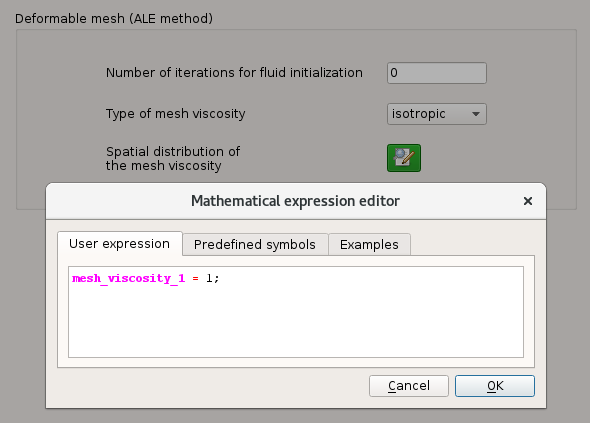
\includegraphics[width=12cm]{gui_ale_mei}
\caption{Thermophysical models - mobile mesh (ALE method)}
\label{fig:Ini-ale}
\end{center}
\end{figure}

The following paragraphs are relevant if the GUI is not used.

\minititre{Function \texttt{cs\_user\_model}}
\noindent
\textit{Function called at the beginning.}
This function completes \texttt{cs\_user\_parameters.c}.

\texttt{cs\_user\_model} allows setting options for the ALE module, and in
particular to activate the ALE module (\texttt{cs\_glob\_ale = CS\_ALE\_LEGACY}).

\minititre{Function \texttt{usstr1}}

This function reads in \texttt{cs\_user\_fluid\_structure\_interaction.f90}. It allows to specify the following pieces of information for the structure module:
\begin{list}{-}{}
  \item the index of the structure, (\texttt{idfstr(ifac)} where \texttt{ifac} is the index of the face). Then the total number of structures \texttt{nbstru} is automatically computed by the code. Be careful, the value must belong to 1, ..., \texttt{nbstru}.
  \item the initial value of displacement, velocity and acceleration
    (\texttt{xstr0}, \texttt{xstreq} and \texttt{vstr0}).
\end{list}

Below is a list of the different variables that might be modified:

\begin{list}{$\bullet$}{}

\item{\texttt{idfstr(ifac)}} \\
{the index of the structure, (\texttt{idfstr(ifac)} where \texttt{ifac} is the index of the face), 0 if the face is not coupled to any structure.}

\item{\texttt{xstr0(i,k)}} \\
{initial position of a structure, where \texttt{i} is the dimension of space
and \texttt{k} the index of the structure}

\item{\texttt{xstreq(i,k)}} \\
{equilibrum position of a structure, where \texttt{i} is the dimension of space
and \texttt{k} the index of the structure}

\item{\texttt{vstr0(i,k)}} \\
{initial velicity of a structure, where \texttt{i} is the dimension of space
and \texttt{k} the index of the structure }
\end{list}

%==================================
\subsubsection{Mesh velocity boundary conditions}
%==================================
These boundary conditions can be managed through the Graphical User Interface (GUI)
 or using the function \texttt{usalcl} (called at each time step). With the GUI,
 when the item ``Deformable mesh'' is selected in ``Calculation features''
 the item ``coupling parameters'' appears under the heading ``Boundary conditions''.
 The user can choose a boundary condition type for ALE (internal coupling) see \figurename~
 \ref{fig:CL-ale1} and \figurename~\ref{fig:CL-ale2}.


\begin{figure}[ht]
\begin{center}
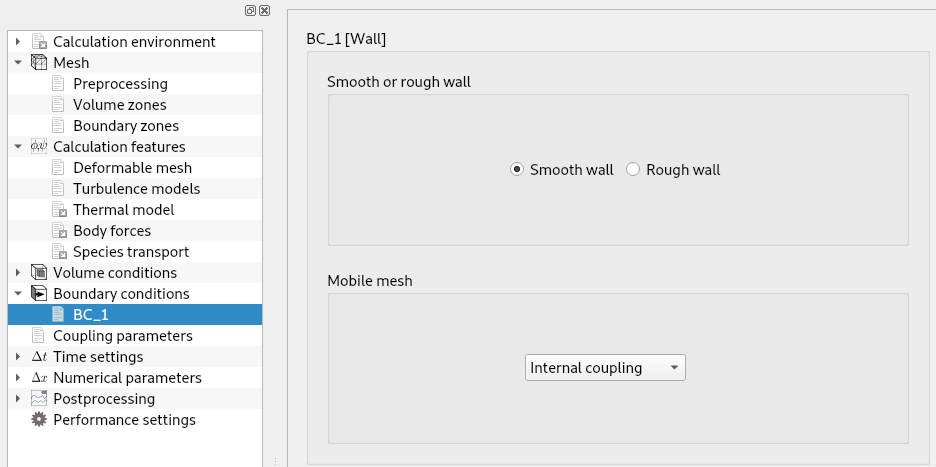
\includegraphics[width=0.9\textwidth]{gui_ale_internal_bc_add}
\caption{Boundary conditions - internal coupling actived}
\label{fig:CL-ale1}
\end{center}
\end{figure}

\begin{figure}[ht]
\begin{center}
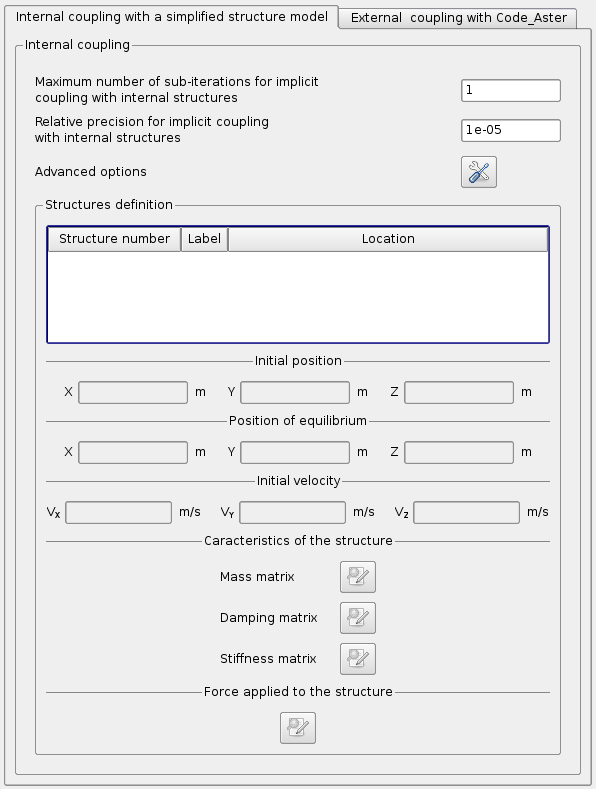
\includegraphics[width=0.9\textwidth]{gui_ale_internal}
\caption{Boundary conditions - internal coupling}
\label{fig:CL-ale2}
\end{center}
\end{figure}

\minititre{Function \texttt{usalcl}}
When the GUI is not used, the use of \texttt{usalcl} is mandatory to run
a calculation using
the ale module just as it is in \texttt{cs\_user\_parameters.f90}. It is used the same way as
\texttt{cs\_user\_boundary\_conditions} in the framework of
standard calculations, that is to say a loop on the boundary faces
marked out by their colour (or more generally by a property of their
family), where the type of mesh velocity boundary condition is definied for
each variable.

The main numerical variables are described below.

\variab{ialtyb}{ialtyb(nfabor)}{ia}{In the ale module, the user
defines the mesh velocity from the colour of the boundary faces, or
more generally from their properties (colours, groups, ...), from the
boundary conditions defined in \texttt{cs\_user\_boundary\_conditions}, or even from their
coordinates. To do so, the array \texttt{ialtyb(nfabor)} gives for each face
\texttt{ifac} the mesh velocity boundary condition types marked out by the key
words \texttt{ivimpo\index{ivimpo}}, \texttt{igliss\index{igliss}},
\texttt{ibfixe\index{ibfixe}} or \texttt{ifresf\index{ifresf}}}.

\begin{list}{$\bullet$}{}

\item If \texttt{ialtyb(ifac) = ivimpo}: imposed velocity.

\begin{list}{$\rightarrow$}{}
\item In the cases where all the nodes of a face have a imposed displacement,
 it is not necessary to fill the tables with mesh velocity boundary conditions
 for this face, these will be erased. In the other case,
 the value of the Dirichlet must be given in \texttt{rcodcl(ifac,ivar,1)} for
 every value of \texttt{ivar} (\texttt{iuma}, \texttt{ivma} and \texttt{iwma}).
 The other boxes of \texttt{rcodcl} and \texttt{icodcl} are completed automatically.

 The tangential mesh velocity is taken like a tape speed under the
 boundary conditions of wall for the fluid, except if wall fluid velocity
 was specified by the user in the interface or \texttt{cs\_user\_boundary\_conditions} (in which case
 it is this speed which is considered).
\end{list}

 \item if \texttt{ialtyb(ifac) = ibfixe}: fixed wall
\begin{list}{$\rightarrow$}{}
 \item the velocity is null.
\end{list}

 \item if \texttt{ialtyb(ifac) = igliss}: sliding wall
\begin{list}{$\rightarrow$}{}
\item symmetry boundary condition on the mesh velocity vector, which means a homogeneous Neumann on the tangential mesh velocity and a zero Dirichlet on the normal mesh velocity.
\end{list}

 \item if \texttt{ialtyb(ifac) = ifresf}: free-surface
\begin{list}{$\rightarrow$}{}
\item an imposed mesh velocity such that the fluid mass flux is equal to the mesh displacement in order to mimic the free-surface automatically. Note that the boundary condition on the fluid velocity must be set separately (homogeneous Neumann condition for instance).
\end{list}

\end{list}

%==================================
\subsubsection{Modification of the mesh viscosity}
%==================================

The user function \texttt{cs\_user\_physical\_properties} can be used along the ALE (Arbitrary Lagrangian Eulerian
 Method) module, and allows modifying the mesh viscosity.
 It is called before the time loop, and before reading restart files
 (so the mesh is always in its initial position at this stage).
The user can modify mesh viscosity values to prevent cells and nodes from huge
 displacements in awkward areas, such as boundary layer for example.

Note that for more complex settings, the mesh viscosity could be modified in
 \texttt{cs\_user\_initialization} or \texttt{cs\_user\_extra\_operations}.
 The matching field's name is \texttt{mesh\_viscosity}.

%==================================
\subsubsection{Fluid - Structure internal coupling}\label{sec:ALE}
%==================================

In the function \texttt{cs\_user\_fluid\_structure\_interaction} the user provides the parameters of two other functions.
\texttt{usstr1} is called at the beginning of the calculation. It is used to define
 and initialise the internal structures where fluid-Structure coupling occurs.
For each boundary face \texttt{ifac}, \texttt{idfstr(ifac)} is the index of the structure
 the face belongs to (if \texttt{idfstr(ifac)} = 0, the face \texttt{ifac} doesn't belong
 to any structure). When using internal coupling, structure index necessarily must be
 strictly positive and smaller than the number of structures. The number of "internal" structures is automatically defined with the maximum
 value of the \texttt{idfstr} table, meaning that internal structure numbers must be defined
 sequentially with positive values, beginning with integer value '1'.

For each internal structure the user can define:
\begin{list}{-}{}
 \item an initial velocity \texttt{vstr0}
 \item an initial displacement \texttt{xstr0} ({\em i.e.} \texttt{xstr0} is the value of the
 displacement \texttt{xstr} compared to the initial mesh at time t = 0)
 \item a displacement compared to equilibrium  \texttt{xstreq} (i.e. \texttt{xstreq}
 is the initial displacement of the internal structure compared to its position at
 equilibrium; at each time step t and for a displacement \text{xstr}(t), the associated
 internal structure will undergo a force $-k*(\text{}t+XSTREQ)$ due to the spring).
\end{list}
\text{xstr0} and \text{vstr0} are initialised with the value 0.
When starting a calculation using ALE, or re-starting a calculation with ALE, based
 on a first calculation without ALE, an initial iteration 0 is automatically performed
 in order to take initial arrays \text{xstr0}, \text{vstr0} and \text{xstreq} into
 account. In any other case, add the following expression '\text{italin=1}' in function
 \text{usipsu}, so that the code can deal with the arrays \text{xstr0}, \text{vstr0} and \text{xstreq}.

When \texttt{ihistr} is set to 1, the code writes in the output the history of the
 displacement, of the structural velocity, of the structural acceleration and of the
 fluid force. The value of structural history output step is the same as the one for
 standard variables \text{nthist}.

The second function, \text{usstr2}, is called at each iteration. One defines in this
 function structural parameters (considered as potentially time dependent): {\em i.e.},
 mass m \text{xmstru}, friction coefficients c \text{xcstru}, and stiffness k \text{xkstru}.
 \text{forstr} array gives fluid stresses acting on each internal structure. Moreover it is also
 possible to take external forces (gravity for example ) into account.
\begin{list}{.}{}
 \item the \text{xstr} array indicates the displacement of the structure compared to its position in the initial mesh,
 \item the \text{xstr0} array gives the displacement of the structures in the initial mesh
 compared to structural equilibrium,
 \item the \text{vstr} array stands for structural velocity.
\end{list}
\text{xstr}, \text{xstr0} and \text{vstr} are \text{DATA} tables that can be used to
 define the  Mass, Friction and Stiffness arays. These are not to be modified.

The 3D structural equation that is solved is the following one:
\begin{equation}\label{eq:FluidStruct}
\displaystyle
\tens{m}.\partial_{tt}\vect{x}+\tens{c}.\partial_{t}\vect{x}+\tens{k}.\left(\vect{x}+\vect{x_0}\right)=\vect{f},
\end{equation}
where $x$ stands for the structural displacement compared to initial mesh position
 \text{xstr}, $x_0$ represents
 the displacement of the structure in initial mesh compared to equilibrium.
Note that $\tens{m}$,$\tens{c}$, and $\tens{k}$ are 3\text{x}3 matrices.
Equation \eqref{eq:FluidStruct} is solved using a Newmark HHT algorithm.
Note that the time step used to solve this equation, \text{dtstr}, can be
 different from the one of fluid calculations. The user is free to define \text{dtstr}
 array. At the beginning of the calculation \text{dtstr} is initialised to the value of
 \text{dtcel} (fluid time step).

%==================================
\subsection{Management of the structure property}
%==================================

The use of \texttt{usstr2} is mandatory to run a calculation using the ALE
 module with a structure module. It is called at each time step.

For each structure, the system that will be solved is:

\begin{equation}
M.x^{''}+C.x^{'}+K.(x-x_{0}) = 0
\end{equation}

where

\begin{list}{-}{}
 \item $M$ is the mass structure (\texttt{xmstru}).
 \item $C$ is the damping coefficient of the structure (\texttt{xcstru}).
 \item $K$ is the spring constant or force constant of the structure (\texttt{xkstru}).
 \item $x_{0}$ is the initial position.
\end{list}

Below is a list of the different variables that might be modified:

\begin{list}{$\bullet$}{}

\item{\texttt{xmstru(i,j,k})} \\
{mass matrix of the structure, where \texttt{i},\texttt{j} is
the array of mass structure and \texttt{k} the index of the structure.}

\item{\texttt{xcstru(i,j,k})}\\
{damping matrix coefficient of the structure, where \texttt{i},\texttt{j} is the array of
damping coefficient and \texttt{k} the index of the structure.}

\item{\texttt{xkstru(i,j,k)}}\\
{spring matrix constant of the structure, where \texttt{i},\texttt{j} is the array of spring
constant and \texttt{k} the index of the structure.}

\item{\texttt{forstr(i,k)}}\\
{force vector of the structure, where \texttt{i} is the force vector and
\texttt{k} the index of the structure.}
\end{list}

%===========================================================
\subsection{Management of the atmospheric module}
%===========================================================

This section describes how to set a calculation using the atmospheric module
of \CS. Each paragraph describes a step of the data setting process.

\subsubsection{Directory structure}\label{sec:atmo_struct}
%
The flowchart (\figurename~\ref{fig:organisation}) recalls the directory
structure of a study generated by \CS .
When using the atmospheric module, the structure is identical but a file called
\texttt{meteo} may be added to the data settings in order to provide vertical
profiles of the main variables. This file should be put in the \texttt{DATA}
directory. For more details about the \texttt{meteo} file, see \S~
~\ref{sec:atmo_BCs}).
%
\begin{figure}[ht]
 \centerline{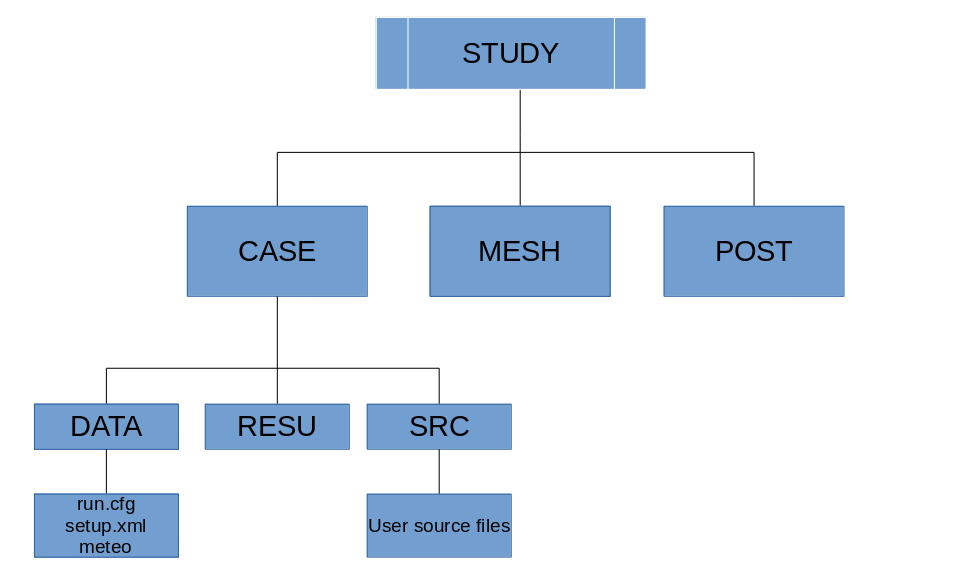
\includegraphics[width=0.99\textwidth]{gui_atmospheric_user_s_guide_v91.png}}
 \caption{Organization of a study (specific files of atmospheric version in bold type)}
 \label{fig:organisation}
\end{figure}
%
\subsubsection{The atmospheric mesh features}
%
An atmospheric mesh has the following specific features:
%
\begin{itemize}
\item The boundary located at the top of the domain should be a plane.
So, horizontal wind speed at a given altitude can be prescribed at the top
face as an inlet boundary.
\item Cells may have very different sizes, from very small (near ground or
buildings) to very large (near the top of domain or far from zone of interest).
\item Vertical resolution: from tiny cells (e.g. $\Delta $\upshape z = 1 m) near
the ground to a few hundreds of meters at the top.
\item Horizontal resolution: from a few meters to hundreds of meters.
\item The length ratio between two adjacent cells (in each direction) should
preferably be between $0.7$ and $1.3$.
\item The z axis represents the vertical axis.
\end{itemize}
%
A topography map can be used to generate a mesh. In this case, the preprocessor
 mode is particularly useful to check the quality of the mesh (run type Mesh
quality criteria).
%
\subsubsection{Atmospheric flow model and steady/unsteady algorithm}
%
The Graphical User Interface (GUI) may be used to enable the atmospheric flow
module and set up the following calculation parameters in the
\texttt{Thermophysical models}-\texttt{Calculation features} page
(see \figurename~\ref{fig:steady}):
%
\subsubsubsection{The atmospheric flow model}
%
The user can choose one of the following atmospheric flow models:
%
\begin{itemize}
\item \textbf{Constant density}: To simulate neutral atmosphere.
\item \textbf{Dry atmosphere}: To simulate dry, thermally-stratified
atmospheric flows (enables \texttt{Potential temperature} as thermal model).
\item \textbf{Humid atmosphere}: To simulate thermally stratified atmospheric
flows (air-water mixture) with phase changes (enables \texttt{Liquid potential
temperature} as thermal model). The model is described in
Bouzereau \cite{bouzereau}.
\end{itemize}
%
\subsubsubsection{The time algorithm}
%
\begin{itemize}
\item Steady flow algorithm: is the one usually set. It sets a time step
variable in space and time. It has to be selected if constant boundary
conditions are used.
\item Unsteady flow algorithm has to be selected for time varying boundary
conditions (the time step can then be variable in time or constant).
\end{itemize}
%
\begin{figure}[ht]
\centerline{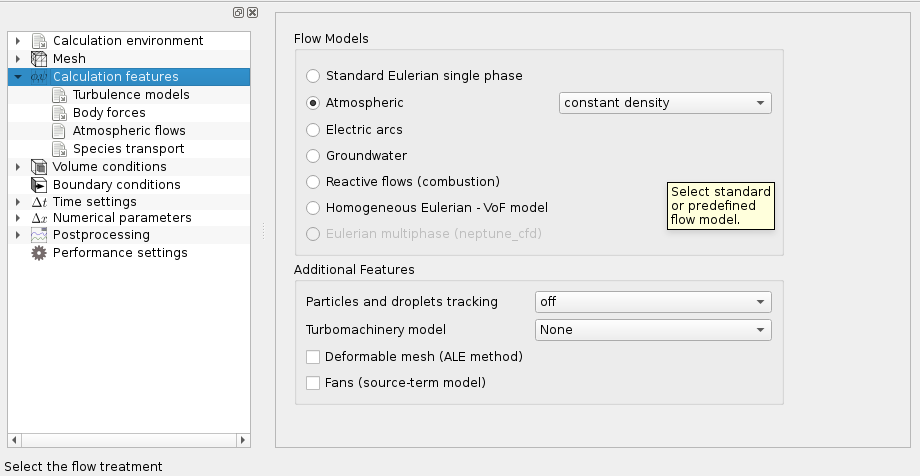
\includegraphics[width=0.7\textwidth]{gui_atmospheric_user_s_guide_v92.png}}
\caption{Selection of atmospheric model}
\label{fig:steady}
\end{figure}
%
\begin{figure}[ht]
\centerline{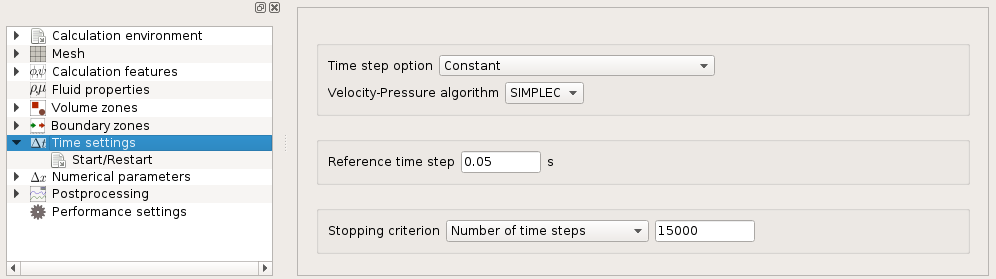
\includegraphics[width=0.9\textwidth]{gui_atmospheric_user_s_guide_v93.png}}
\caption{Selection of steady/unsteady flow algorithm}
\label{fig:global}
\end{figure}
%
Table \tablename~\ref{tab:param_list} can help to choose the right parameters
depending on the type of atmospheric flow.
%
\subsubsubsection{Warnings}
The following points have to be considered when setting the parameters
described above:
\begin{itemize}
\item The potential temperature thermal model and the liquid potential
temperature one (see the paragraph ``Atmospheric main variables'' for the
definition) requires that the vertical component of the gravity is set to
$g_z=-9.81 m.s^{-2}$ ($g_x=g_y=0 m.s^{-2}$),
otherwise pressure and density won't be correctly computed.
\item As well, the use of scalar with drift for atmospheric dispersion requires
the gravity to be set to $g_z=-9.81$ ($g_x=g_y=0 m.s^{-2}$), even if the density
is constant.
\end{itemize}
%
\subsubsection{Physical properties}
%
The specific heat value has to be set to the atmospheric value
$C_{p}=1005 J/kg/K$.
%
\begin{table}[ht]\label{tab:param_list}
\begin{center}
\begin{tabular}{|p{80pt}|p{70pt}|p{70pt}|p{80pt}|p{100pt}|}
\hline
\textbf{Parameters} & \textbf{Constant density} & \textbf{Dry atmosphere} & \textbf{Humid atmosphere} & \textbf{Explanation} \\
\hline
pressure boundary condition & Neumann first order & Extrapolation & Extrapolation &
In case of \textbf{Extrapolation}, the pressure gradient is assumed (and set) constant, whereas in case of \textbf{Neumann first order},
the pressure gradient is assumed (and set) to zero. \\
\hline
Improved pressure interpolation in stratified flows & no & yes & yes & If yes, exact balance between the hydrostatic part of the pressure gradient and the gravity term $\rho g$ is numerically ensured. \\
\hline
Gravity (gravity is assumed aligned with the z-axis) & $g_z=0$ or $g_z=-9.81 m.s^{-2}$ (the latter is useful for scalar with drift) & $g_z=-9.81 m.s^{-2}$ & $g_z=-9.81 m.s^{-2}$ &  \\
\hline
Thermal variable & no & potential temperature & liquid potential temperature &  \\
\hline
Others variables & no & no & total water content, droplets number &  \\
\hline
\end{tabular}\label{tab1}
\caption[List of parameters]{List of parameters}
\end{center}
\end{table}
%
\subsubsection{Boundary and initial conditions}\label{sec:atmo_BCs}
%
The \texttt{meteo} file can be used to define initial conditions for the
different fields and to set up the inlet boundary conditions. For the velocity
field, \CS can automatically detect if the boundary is an inlet boundary or an
outflow boundary, according to the wind speed components given in the
\texttt{meteo} file with respect to the boundary face orientation. This is often
used for the lateral boundaries of the atmospheric domain, especially if the
profile is evolving in time. In the case of inlet flow, the data given in the
\texttt{meteo} file will be used as the input data (Dirichlet boundary condition)
for velocity, temperature, humidity and turbulent variables. In the case of
outflow, a Neumann boundary condition is automatically imposed (except for the
pressure). The unit of temperature in the \texttt{meteo} file is the degree
Celsius whereas the unit in the GUI is the kelvin.

To be taken into account, the \texttt{meteo} file has to be selected in the GUI
(\texttt{Atmospheric flows} page, see \figurename~\ref{fig:meteo}) and the check
box on the side ticked. This file gives the profiles of prognostic atmospheric
variables containing one or a list of time stamps. The file has to be put in the
\texttt{DATA} directory.
%
\begin{figure}[htbp]
\centerline{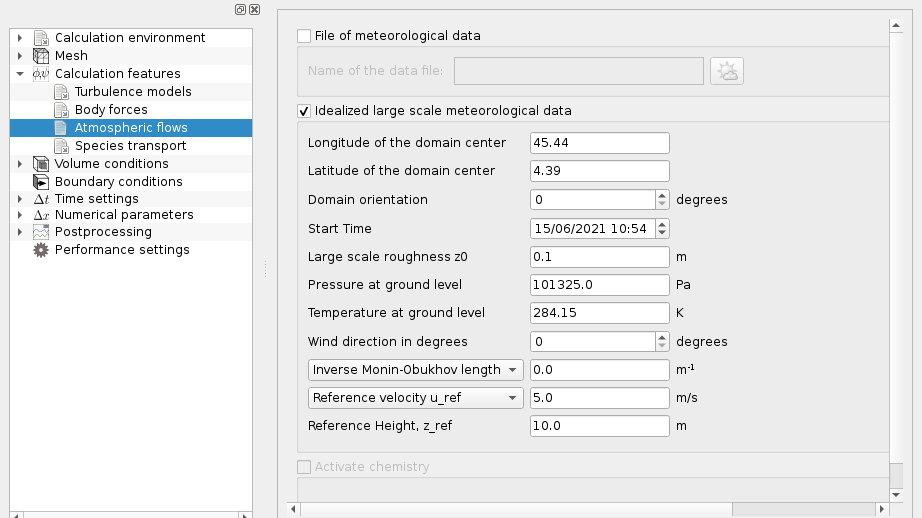
\includegraphics[width=0.9\textwidth]{gui_atmo_read.png}}
\caption{Selection of the \texttt{meteo} file}
\label{fig:meteo}
\end{figure}
%
An example of file \texttt{meteo} is given in the directory
\texttt{data/user/meteo}. The file format has to be strictly respected.
The horizontal coordinates are not used at the present time (except when
boundary conditions are based on several meteorological vertical profiles)
and the vertical profiles are defined with the altitude above sea level. The
highest altitude of the profile should be above the top of the simulation domain
and the lowest altitude of the profile should be below or equal to the lowest
level of the simulation domain. The line at the end of the \texttt{meteo} file
should not be empty.

If the boundary conditions are variable in time, the vertical profiles for
the different time stamps have to be written sequentially in the \texttt{meteo}
file.

You can also set the profiles of atmospheric variables directly in the GUI.
The following boundary conditions can be selected in the GUI:
%
\begin{itemize}
\item Inlet/Outlet is automatically calculated for lateral boundaries
(e.g. North, West\textellipsis ) of the computational domain
(see \figurename~\ref{fig:inlet}).
\item Inlet for the top of the domain (see \figurename~\ref{fig:top}).
\item Rough wall for building walls (see \figurename~\ref{fig:walls}) or for
the ground (see \figurename~\ref{fig:ground}).
The user has to enter the roughness length. In case of variable roughness
length, the user has to provide the land use data and the association
between the roughness length values and land use categories.
\end{itemize}
%
\begin{figure}[htbp]
\centerline{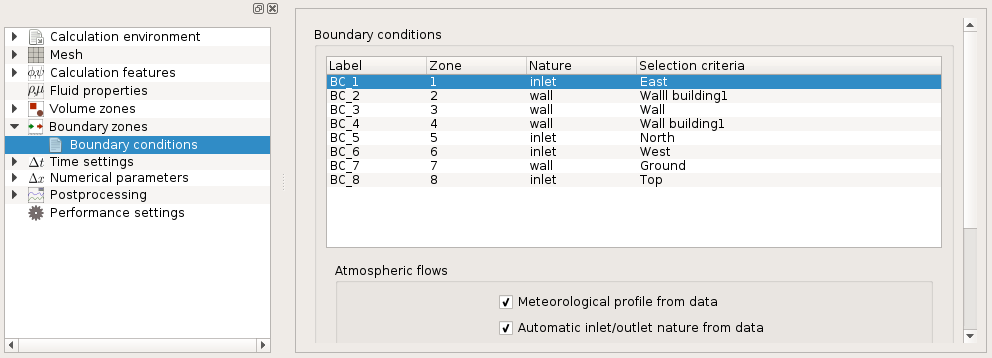
\includegraphics[width=0.9\textwidth]{gui_atmospheric_user_s_guide_v95.png}}
\caption{Selection of automatic inlet/ outlet for boundary conditions }
\label{fig:inlet}
\end{figure}
%
\begin{figure}[htbp]
\centerline{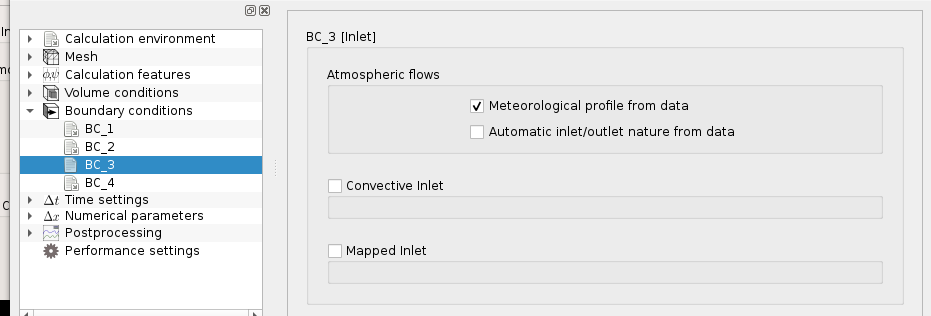
\includegraphics[width=0.9\textwidth]{gui_atmospheric_user_s_guide_v96.png}}
\caption{Selection of the boundary condition for the top of the domain }
\label{fig:top}
\end{figure}
%
\begin{figure}[htbp]
\centerline{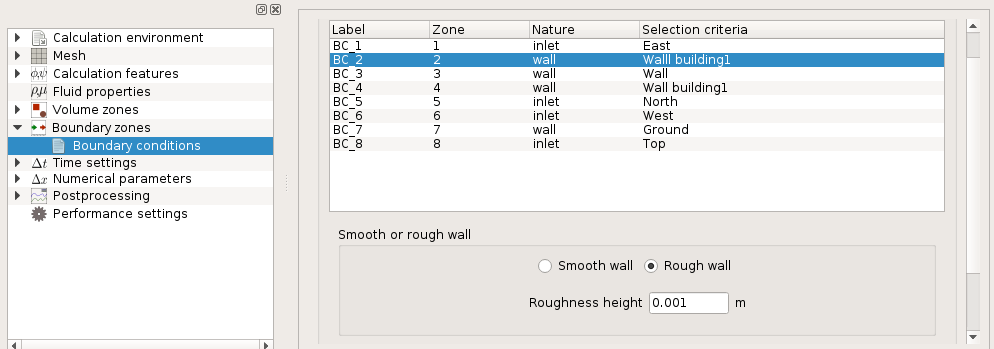
\includegraphics[width=0.9\textwidth]{gui_atmospheric_user_s_guide_v97.png}}
\caption{Selection of the boundary condition for building walls}
\label{fig:walls}
\end{figure}
%
\begin{figure}[htbp]
\centerline{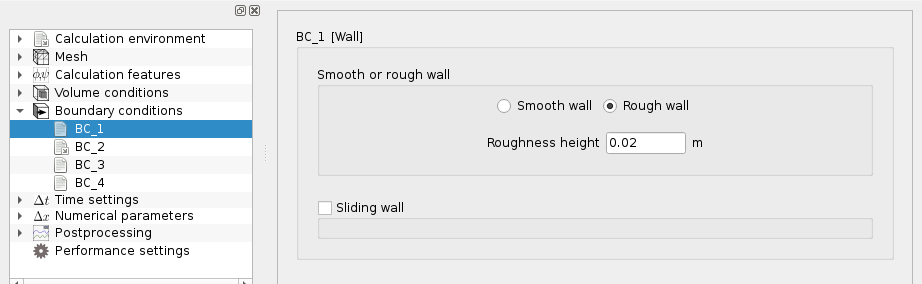
\includegraphics[width=0.9\textwidth]{gui_atmospheric_user_s_guide_v98.png}}
\caption{Selection of the boundary condition for the ground}
\label{fig:ground}
\end{figure}

\paragraph{Remark:} If a meteorological file is given, it is used by default to
initialize the variables. If a meteorological file is not given, the user can
use the standard \CS initial and boundary conditions set up but has to be aware
that even small inconsistencies can create very large buoyancy forces and
spurious circulations.

\subsubsubsection{Boundary conditions based on several meteorological vertical profiles}

In some cases, especially when outputs of a mesoscale model are used, you
need to build input boundary conditions from several meteorological vertical
wind profiles. Cressman interpolation is then used to create the boundary
conditions. The following files need to be put in the \texttt{DATA} directory:
\begin{itemize}
\item All \texttt{meteo} files giving the different vertical profiles of
prognostic variables (wind, temperature, turbulent kinetic energy and
dissipation).
\item A file called \texttt{imbrication\_files\_list.txt} which is a list
of the \texttt{meteo} files used.
\item A separate \texttt{meteo} file which is used for the initial conditions
and to impose inlet boundary conditions for the variables for which Cressman
interpolation is not used (for example: temperature, turbulent kinetic energy).
This file must follow the rules indicated previously.
\end{itemize}
The following files should be put in the SRC directory:
\begin{itemize}
\item The user source file \texttt{cs\_user\_parameters.f90}. In this file, set
the \texttt{cressman\_} flag of each variable, for which the Cressman
interpolation should be enabled, to \texttt{.true.}.
\end{itemize}
%
\subsubsection{User functions}
%
The user functions are used when the graphical user interface is not
sufficient to set up the calculation. We give some examples of user file for
atmospheric application:
\begin{itemize}
\item \texttt{cs\_user\_source\_terms.c}: to add a source term in the
prognostic equations for forest canopy modelling, wind turbine wake modelling...
%See the associated \doxygenfile{cs_user_source_terms.html}{\texttt{doxygen} documentation}.
for examples of use of \texttt{cs\_user\_source\_terms.c}.
\item \texttt{cs\_user\_parameters.f90}: to activate the Cressman interpolation.
For example, it is used to impose inhomogeneous boundary conditions.% See the associated
%\doxygenfile{f_parameters.html}{\texttt{doxygen} documentation}.
for examples of use of \texttt{cs\_user\_parameters.f90}.
\item \texttt{cs\_user\_extra\_operations.c}: to generate vertical
profiles for post processing. %See the associated
%\doxygenfile{cs_user_extra_operations_examples.html}{\texttt{doxygen} documentation}.
for examples of use of \texttt{cs\_user\_extra\_operations-mean\_profiles.c}
\item \texttt{cs\_user\_boundary\_conditions.f90}: show how to set
up the boundary conditions and to put a heterogeneous roughness length...
%See the associated \doxygenfile{cs_user_boundary_conditions_examples.html}{\texttt{doxygen}
%documentation}.
for examples of use of \texttt{cs\_user\_boundary\_conditions-atmospheric.f90}.
\end{itemize}
%
\paragraph{Remark:}
If the computation is set without the GUI, other user functions such as the
following have to be used:
\begin{itemize}
\item \texttt{cs\_user\_initialization.c}: allows to initialize
or modify (in case of a restarted calculation) the calculation variables and
the values of the time step. %See the associated \doxygenfile{user_initialization.html}{\texttt{doxygen} documentation}.
\\for examples of use of \texttt{cs\_user\_initialization-atmospheric.c}
\item \texttt{cs\_user\_boundary\_conditions-atmospheric.f90}: allows to define
all the boundary conditions. For each type of boundary condition, faces should
be grouped as physical zones characterized by an arbitrary number \texttt{izone}
chosen by the user. If a boundary condition is retrieved from a meteorological
profile, the variable \texttt{iprofm(izone)} of the zone has to be set to 1.
The vertical profiles of atmospheric variables can be described in this file.
\end{itemize}
%
Examples are available in the directory \texttt{SRC/USER\_EXAMPLE}.
%
\subsubsection{Physical models}
%
\subsubsubsection{Atmospheric dispersion of pollutants}
%
To simulate the atmospheric dispersion of pollutant, one first need to define
the source(s) term(s). That is to say the location i.e. the list of cells or
boundary faces, the total air flow, the emitted mass fraction of pollutant,
the emission temperature and the speed with the associated turbulent parameters.
The mass fraction of pollutant is simulated through a user added scalar that
could be a `scalar with drift' if wanted (aerosols for example).

The simulations can be done using 3 different methods:
\begin{enumerate}
\item Using a mass source term, that is added in the Navier-Stokes
equations using the \texttt{cs\_user\_mass\_source\_terms.f90} user function.

\item Prescribing a boundary condition code ``total imposed mass flux`` for
some boundary faces using the \texttt{cs\_user\_boundary\_conditions.f90} user
function.

\item Using a scalar source term. In this case, the air inflow is not taken
into account. The user has to add an explicit part to the equations
for the scalar through the \texttt{cs\_user\_source\_terms.c} file. This is
done by selecting the cells and adding the source term \texttt{st\_exp (cells)}
which equals to the air flux multiplied by the mass fraction, while the
implicit part \texttt{st\_imp} is set to zero.
\end{enumerate}

The first method is recommended, but one must take care that each source
influences the dispersion of the others, which is physically realistic. So
if the impact of several sources has to be analyzed independently it has first
to be verified that these influences are negligible or as many simulations
as there are sources have to be run.

With the second method, the same problem of sources interactions appears, and
moreover standard Dirichlet conditions should not be used (use
\texttt{itypfb=i\_convective\_inlet} and \texttt{icodcl=13} instead) as
the exact emission rate cannot be prescribed because the diffusive part
(usually negligible) cannot be quantified. Additionally, it requires that
the boundary faces of the emission are explicitly represented in the mesh.

Finally the third method does not take into account the jet effect of the
emission and so must be used only if it is sure that the emission does not
modify the flow.

Whatever solution is chosen, the mass conservation should be verified by using
for example the
\texttt{cs\_user\_extra\_operations-scalar\_balance.c} file.

\subsubsubsection{Soil/atmosphere interaction model}

This model is based on the force restore model (Deardorff \cite{deardorff}).
It takes into account heat and humidity exchanges between the ground and the
atmosphere at daily scale and the time evolution of ground surface temperature
and humidity. Surface temperature is calculated with a prognostic equation
whereas a 2-layers model is used to compute surface humidity.

The parameter \texttt{iatsoil} in the file \texttt{atini0.f90} needs to be equal to one to
activate the model. Then, the source file \texttt{solvar.f90} is used.

Three variables need to be initialized in the file \texttt{atini0.f90}: deep soil
temperature, surface temperature and humidity.

The user needs to give the values of the model constants in the file
\texttt{solcat.f90}: roughness length, albedo, emissivity...

In case of a 3D simulation domain, land use data has to be provided for the domain.
Values of model constants for the land use categories have also to be
provided.

\subsubsubsection{Radiative model (1D)}

The 1D-radiative model calculates the radiative exchange between different
atmospheric layers and the surface radiative fluxes.

The radiative exchange is computed separately for two wave lengths intervals

\begin{itemize}
\item Calculation in the infrared spectral domain (file \texttt{rayir.f90})
\item Calculation in the spectral range of solar radiation (file
\texttt{rayso.f90})
\end{itemize}
This 1D-radiative model is needed if the soil/atmosphere interaction model
is activated.

This model is activated if the parameter \texttt{iatra1} is equal to one in the
file \texttt{cs\_users\_parameters.f90}.

\subsubsection{Atmospheric main variables}

For more details on the topic of atmospheric boundary layers, see  Stull
\cite{stull}.
%
\begin{itemize}
\item Definition of the potential temperature:
\[
\theta =T\left(\frac{P}{P_{r}}\right)^{-\frac{R_{d}}{C_{p}}}
\]
\item Definition of liquid potential temperature:
\[
\theta_{l} = \theta \left( 1-\frac{L}{C_{p}T} q_{l} \right)
\]
\item Definition of virtual temperature:
\[
T_{v} = \left(1+0.61q\right)T
\]
\item Gas law:
\[
P = \rho \frac{R}{M_{d}}\left(1+0,61q\right)T
\]
with $R=R_{d} M_{d}$.
\item Hydrostatic state:
\[
\frac{\partial P}{\partial z} = -\rho g
\]
\end{itemize}
%
\begin{table}[htbp]
\begin{center}
\begin{tabular}{|l|l|l|l|}
\hline
\textbf{Constant name} & \textbf{Symbol} & \textbf{Values} & \textbf{Unit} \\
\hline
Gravity acceleration at sea level & $g$ & $9.81$ & $m.s^{-2}$ \\
\hline
Effective Molecular Mass for dry air & $M_{d}$ & $28.97$ & $kg.kmol^{-1}$ \\
\hline
Standard reference pressure & $P_{r}$ & $10^{5}$ & $Pa$ \\
\hline
Universal gas constant & $R$ & $8.3143$ & $J.K^{-1}.mol$ \\
\hline
Gas constant for dry air & $R_{d}$ & $287$ & $J.kg^{-1}.K^{-1}$ \\
\hline
\end{tabular}\label{tab2}
\end{center}
\caption{Constant name}
\end{table}

\begin{table}[htbp]
\begin{center}
\begin{tabular}{|l|p{113pt}|}
\hline
\textbf{Variable name} &\textbf{Symbol} \\
\hline
Specific heat capacity of dry air & $C_{p}$ \\
\hline
Atmospheric pressure & $P$ \\
\hline
Specific humidity & $q$ \\
\hline
Specific content for liquid water & $q_{l}$ \\
\hline
Temperature & $T$ \\
\hline
Virtual temperature & $T_{v}$ \\
\hline
Potential temperature & $\theta$ \\
\hline
Liquid potential temperature & $\theta_{l}$ \\
\hline
Latent heat of vaporization & $L$ \\
\hline
Density & $\rho $ \\
\hline
Altitude & $z$ \\
\hline
\end{tabular}\label{tab3}
\caption{Variable name}
\end{center}
\end{table}
%
\subsubsection{Recommendations}\label{subsubsec:recommendations}
%
This part is a list of recommendations for atmospheric numerical simulations.
%
\begin{itemize}
\item Enough probes at different vertical levels in the domain should be used
to check the convergence of the calculation.
\item An inflow boundary condition at the top level of the domain should be set
(symmetry and automatic inlet/outlet are not appropriate).
\item A Courant number too small or too big has to be avoided (see \CS Best
Practice Guidelines). That is the reason why the option \texttt{variable time
step in space and in time} is recommended for steady simulations when there are
large differences of cell size inside the domain (which is generally the case
for atmospheric simulations). With this option, it can be necessary to change
the reference time step and the time step maximal increase (by default, the time
step increase rate is $10\%$).
\end{itemize}
%
In some cases, results can be improved with the following modifications:
%
\begin{itemize}
\item In some case, the turbulent eddy viscosity can drop to unrealistically low
values (especially with $k-\varepsilon$ model in stable atmospheric condition).
In those cases, it is suggested to put an artificial molecular viscosity around
$0.1 m^{2}.s^{-1}$.
\item If the main direction of wind is parallel to the boundary of your computing
domain, try to set symmetry boundary conditions for the lateral boundaries to
avoid inflow and outflow on the same boundary zone (side of your domain).
Another possibility is to use a cylindrical mesh.
\item To avoid inflow and outflow on the same boundary zone (side of your domain),
avoid the case of vertical profile in the input data \texttt{meteo} file with
changes of the sign of velocity of wind ($V_x$ or/and $V_y$).
\end{itemize}

%==================================
%\subsection{Cooling tower modelling}
%==================================

%==================================
%\subsubsection{Parameters}
%==================================

%\noindent
%\textit{Function called only during calculation initialisation? OR AT EACH ITERATION?.}

%The function \texttt{uscti1} contains calculation parameters such as:
%\begin{list}{-}{}
% \item  temperature parameters,
% \item  the number of exchange zones at various locations,
% \item  the air properties.
%\end{list}

%==================================
%\subsubsection{Initialisation of the variables}
%==================================

%With the additional variables introduced with the air-cooling module, the
%following quantities may be initialized by  \texttt{cs\_user\_initialization} in
%user selected zones in addition to the usual quantities:
%\begin{list}{-}{}
% \item the air temperature, variable of index \texttt{isca(ihumid)},
% \item the air humidity, variable of index \texttt{isca(itemp4)},
%\end{list}
%where \texttt{iel} can be an element found in a list returned by the routine
% '\texttt{getcel}'.

%==================================
%\subsubsection{Definition of the exchange zones}
%==================================

%The function \texttt{usctdz} is used to define the exchange zones of a cooling
% tower. The user provides the following parameters:
%\begin{list}{-}{}
% \item \texttt{imzech}: its value is related to the model used:
%      \begin{list}{$\rightarrow$}{}
%       \item 0: no model is used,
%       \item 1: Merkel model is used,
%       \item 2: Poppe model is used,
%      \end{list}
% \item 10 exchange zone parameters.
%\end{list}
%These arguments are passed to the function '\texttt{defct}' along with a
%geometrical selection criterion.

%==================================
\subsection{Turbomachinery computations}
%==================================

\subsubsection{Introduction}

Two classical models are available in \CS for rotor/stator
interactions modelling in turbomachinery computations: the steady
approach which is based on the so-called \emph{Frozen Rotor} modelling
and the \emph{transient rotor/stator} approach which is based on a
sliding mesh technique.

\underline{\emph{Warning:}} This section describes these functionalities based on
a single \CS computation. An alternative rotor/stator coupling based
on coupling of boundary conditions is also possible (and only briefly
described in this section) but it is not recommended.

\subsubsection{Meshing reccomendations}\label{tbm_mesh}

\paragraph{Periodicity}\label{tbm_mesh_perio}

The rotational periodicity treatment is possible only in \emph{Frozen
Rotor}. However, the interface plane between rotor and stator
must match in the azimutal $\theta$ direction:
$$\theta_{\text{min}}^{\text{rotor}}(z)=\theta_{\text{min}}^{\text{stator}}(z),\quad\theta_{\text{max}}^{\text{rotor}}(z)=\theta_{\text{max}}^{\text{stator}}(z)$$
for all $z$ through the rotation axis direction.

\paragraph{Rotor/stator interface}\label{tbm_mesh_interface}
\begin{itemize}
\item \emph{Unsteady rotor/stator}: in the input mesh(es), the
  interface between rotor and stator domains has to be composed of
  \underline{boundary faces}. Then the interface boundary faces are joined
  during the computation and become internal faces, as is usual for
  mesh joining in the preprocessing stage. A simple way to ensure
  joining is not done prematurely is to provide
  \underline{separated meshes} for each rotor or stator domain.
\item \emph{Frozen Rotor}: the interface can be composed of boundary
   faces (in which case the interface boundary faces are joined at
   the beginning of the computation) or of internal faces.
\end{itemize}

\paragraph{Meshing of the interface region}\label{tbm_user_bpg_mesh}

As mentioned above, when a rotor/stator interface boundary exists (in
particular for the \emph{unsteady rotor/stator} model), boundary faces
are joined by the solver during the computation, based on the current
rotor position. It is thus important to be aware that the success of
a joining operation is strongly dependant on the
\underline{quality of the mesh at the interface}. More precisely,
the refinement must be as similar as possible at both sides of the
interface. Moreover, it is reminded that the tolerance parameter of
a joining is a fraction of the shortest edge linked with a vertex of
a joined face. Consequently, cells with high aspect ratios where the
refinement in the azimutal $\theta$ direction is much coarser than
those in one of the two others can also lead to a joining failure.
In particular, the user should be careful to avoid elongated
viscous layer type cells in curved areas such as a rotor-stator interface.

If the meshes at both sides of the interface are very different
such that the joining fails, advanced joining parameters are
available. However, modifying the mesh is more likely to
succeed. The introduction of a somekind of buffer cells layer on
both sides of the interface should be very valuable. Ideally, each
of the two layers should have the same refinement and a constant
azimutal step (this latter recommandation is relevant only for
\emph{unsteady rotor/stator} model).

\paragraph{Alternative rotor/stator coupling}\label{tbm_user_bpg_cpl}

If the meshes at both sides of the interface are very different and
can not be modified, a fallback solution is to use the rotor/stator model
based on the boundary conditions coupling.

\underline{\emph{Warning:}} Contrarily to the mesh joining approach, the
boundary conditions coupling approach is not fully conservative.

\subsubsection{Turbomachinery dedicated postprocessing functions}\label{tbm_user_post}

Useful postprocessing functions relative to the machinery
characteristics are available: postprocessing of the couple on the
rotor walls and postprocessing of the head generated by the machinery.

\subsubsection{Data setting, keywords and examples}\label{tbm_date_setting}
Data setting, keywords and examples for turbomachinery computations
(mesh joining or boundary conditions coupling), are provided in
\doxygenfile{turbomachinery.html}{the dedicated \texttt{doxygen}
documentation}.

%==================================
\subsection{Cavitation module}
%==================================

The cavitation module is based on an homogeneous mixture model. The
physical properties (density and dynamic viscosity) of the mixture
depends on a resolved void fraction and constant reference properties
of the liquid phase and the gas phase.

For a description of the user management of the cavitation module,
please refer to \doxygenfile{cavit.html}{the dedicated
  \texttt{doxygen} documentation}.

%-------------------------------------------------------------------------------

% This file is part of Code_Saturne, a general-purpose CFD tool.
%
% Copyright (C) 1998-2012 EDF S.A.
%
% This program is free software; you can redistribute it and/or modify it under
% the terms of the GNU General Public License as published by the Free Software
% Foundation; either version 2 of the License, or (at your option) any later
% version.
%
% This program is distributed in the hope that it will be useful, but WITHOUT
% ANY WARRANTY; without even the implied warranty of MERCHANTABILITY or FITNESS
% FOR A PARTICULAR PURPOSE.  See the GNU General Public License for more
% details.
%
% You should have received a copy of the GNU General Public License along with
% this program; if not, write to the Free Software Foundation, Inc., 51 Franklin
% Street, Fifth Floor, Boston, MA 02110-1301, USA.

%-------------------------------------------------------------------------------

%==================================
%==================================
\section{Key word list}
%==================================
%==================================
\label{prg_motscles}

The key words are classified under headings. For each key word of the Kernel of \CS,
the following data are given:

\noindent
\makebox[2.5cm][l]{Variable name}\makebox[1.3cm][l]{Type}%
\makebox[5cm][l]{Allowed values}%
\makebox[4.cm][l]{[Default]}O/C\hspace{1cm}Level\\
\hspace*{2.5cm}Description\\
\hspace*{2.5cm}Potential dependences


\begin{list}{$\bullet$}{}
\item \textbf{Variable name}: Name of the variable containing the key word.

\item \textbf{Type}: a (Array), i (Integer), r (Real number), c
      (Character string).

\item \textbf{Allowed values}: list or range of allowed values.

\item \textbf{Default}: value defined by the code before any user
      modification (every key word has one). In some cases, a
      non-allowed value is given (generally $-999$ or $-10^{12}$), to force the
      user to specify a value. If he does not do it, the code may:
\begin{list}{-}{}
\item automatically use a recommended value (for instance, automatical
      choice of the variables for which chronological records will be
      generated).

\item stop, if the key word is essential (for instance, value of the
      time step).
\end{list}

\item \textbf{O/C}: Optional/Compulsory
\begin{list}{-}{}
\item O: optional key word, whose default value may be enough.

\item C: key word which must imperatively be specified (for instance,
      the time step).
\end{list}

\item \textbf{Level}: L1, L2 or L3
\begin{list}{-}{}
\item L1 (level 1): the users will have to modify it in the framework of
      standard applications. The L1 key words are written in bold.

\item L2 (level 2): the users may have to modify it in the framework of
      advanced applications. The L2 key word are all optional.

\item L3 (level 3): the developers may have to modify it ; it keeps its
      default value in any other case. The L3 key word are all optional.
\end{list}

\item \textbf{Description}:  key word description, with its potential
      dependences.

\end{list}

The L1 key words can be modifed through the Graphical Use Interface or
in the \texttt{cs\_user\_parameters.f90} file. L2 and L3 key words can only be modified through
the \texttt{cs\_user\_parameters.f90} file, even if they do not appear in the version proposed
as example it the \texttt{SRC/REFERENCE/base} directory.\\
It is however recommended not to modify the key words which do not belong to the L1
level.

The alphabetical key word list is displayed in the index, in the end of
this report.

\minititre{Notes}
$\bullet\ $The notation ``d'' refers to a double precision real. For
           instance, 1.8d-2 means 0.018. \\
$\bullet\ $The notation ``{\tt grand}'' (which can be used in the code)
corresponds to $10^{12}$.

%==================================
\subsection{Input-output}
%==================================

\minititre{Notes}
\begin{list}{$\bullet$}{}
\item Two different files can have neither the same unit number nor the
      same name.
\end{list}

%==================================
\subsubsection{''Calculation'' files}
%==================================


\minititre{General}

\motcle{impstp}{i}{strictly positive integer}{12}{O}{L3}
{unit of the calculation interactive stop file\\
always useful (because of the interactive character)}

\motcle{ficstp}{c}{string of 6 characters}{\tt ficstp}{O}{L3}
{name of the calculation interactive stop file (see p.\pageref{prg_ficstp})\\
always useful (because of the interactive characteristic)}

\minititre{1D wall thermal module}

\motcle{ficmt1}{c}{string of 13 characters}{\tt t1damo}{O}{L3}
{name of the upstream restart file for the 1D wall thermal module.\\
useful if and only if {\tt isuit1 = 1} and {\tt nfpt1d$>$0}}

\motcle{ficvt1}{c}{string of 13 characters}{\tt t1dava}{O}{L3}
{name of the upstream restart file for the 1D wall thermal module\\
useful if and only if {\tt nfpt1d$>$0}}

\minititre{Vortex method for LES}

\motcle{impmvo}{i}{strictly positive integer}{\tt impmvo}{O}{L3}
{unit of the upstream restart file for the vortex method\\
useful if and only if {\tt isuivo = 1} and {\tt ivrtex=1}}

\motcle{ficmvo}{c}{string of 13 characters}{\tt voramo}{O}{L3}
{name of the upstream restart file for the vortex method\\
This is always a text file (this file has a different structure from the
other restart files)\\
useful if and only if {\tt isuivo = 1} and {\tt ivrtex=1}}

\motcle{impvvo}{i}{strictly positive integer}{\tt impvvo}{O}{L3}
{unit of the downstream restart file for the vortex method\\
useful if and only if {\tt ivrtex=1}}

\motcle{ficvvo}{c}{string of 13 characters}{\tt vorava}{O}{L3}
{name of the upstream restart file for the vortex method\\
This is always a text file (this file has a different structure from the
other restart files)\\
useful if and only if {\tt ivrtex=1}}

\motcle{impdvo}{i}{strictly positive integer}{\tt impdvo}{O}{L3}
{unit of the {\tt ficvor} data files for the vortex method. These
files are text files. Their number and names are specified by the user in
the \texttt{usvort} subroutine.\\
(Although it corresponds to an ``upstream'' data file, {\tt impdvo} is
initialized to 20 because, in case of multiple vortex entries,
it is opened at the same time as the {\tt ficmvo} upstream restart file,
which already uses unit 11)\\
useful if and only if {\tt ivrtex=1}}


\minititre{Radiation}

\motcle{ficamr}{c}{string of 13 characters}{\tt rayamo}{O}{L3}
{name of the radiation upstream restart file.\\
useful if and only if {\tt isuird = 1}}

\motcle{ficavr}{c}{string of 13 characters}{\tt rayava}{O}{L3}
{name of the radiation downstream restart file \\
always useful in case of radiation modeling}


\minititre{Thermochemistry}

\motcle{impfpp}{i}{strictly positive integer}{25}{O}{L3}
{unit of the thermochemical data file\\
useful in case of gas or pulverised coal combustion or electric arc}

\motcle{ficfpp}{c}{string of 6 characters}{\tt dp\_tch}{O}{L3}
{name of the thermochemical data file. The launch script is designed to copy the
user specified thermochemical data file in the temporary execution directory
under the name \texttt{dp\_tch}, for \CS to open it properly. Should the value
of {\tt ficfpp} be changed, the launch script would have to be adapted.\\
useful in case of gas or pulverised coal combustion}

\motcle{impjnf}{i}{strictly positive integer}{\tt impfpp}{O}{L3}
{unit of the JANAF data file\\
useful in case of gas or pulverised coal combustion}

\motcle{ficjnf}{c}{string of 5 characters}{\tt JANAF}{O}{L3}
{name of the JANAF data file. The launch script is designed to copy the
user specified JANAF data file in the temporary execution directory
under the name \texttt{JANAF}, for \CS to open it properly. Should the value
of {\tt ficjnf} be changed, the launch script would have to be adapted.\\
useful in case of gas or pulverised coal combustion}

\minititre{Lagrangian}

\motcle{ficaml}{c}{string of 6 characters}{\tt lagamo}{O}{L3}
{name of the upstream restart file in case of Lagrangian modeling.\\
useful if and only if {\tt isuila = 1}}

\motcle{ficmls}{c}{string of 13 characters}{\tt lasamo}{O}{L3}
{name of the upstream restart file for the statistics in case of
Lagrangian modeling.\\
useful if and only if {\tt isuist = 1}}

\motcle{ficavl}{c}{string of 13 characters}{\tt lagava}{O}{L3}
{name of the downstream restart file in case of Lagrangian modeling\\
always useful in case of Lagrangian modeling}

\motcle{ficvls}{c}{string of 6 characters}{\tt lasava}{O}{L3}
{name of the downstream restart file for the statistics in case of
Lagrangian modeling\\
useful in case of Lagrangian modeling with statistics}

\motcle{impla1}{i}{strictly positive integer}{50}{O}{L3}
{unit of a file specific to Lagrangian modeling\\
useful in case of Lagrangian modeling}

\motcle{impla2}{i}{strictly positive integer}{51}{O}{L3}
{unit of a file specific to Lagrangian modeling\\
useful in case of Lagrangian modeling}

\motcle{impla3}{i}{strictly positive integer}{52}{O}{L3}
{unit of a file specific to Lagrangian modeling\\
useful in case of Lagrangian modeling}

\motcle{impla4}{i}{strictly positive integer}{53}{O}{L3}
{unit of a file specific to Lagrangian modeling\\
useful in case of Lagrangian modeling}

\motcle{impla5}{ia}{strictly positive integer}{54 to 68}{O}{L3}
{units of files specific Lagrangian modeling, 15-dimension array\\
useful in case of Lagrangian modeling}


%==================================
\subsubsection{Post-processing for {\em EnSight} or other tools}
%==================================

\minititre{Notes}
$\bullet\quad$The format depends on the user choices, and most options
are defined using the GUI or \\
\texttt{cs\_user\_postprocess.c}.\\
$\bullet\quad$The post-processing files can be of the following formats: {\em Ensight Gold},
{\em MED} or {\em CGNS}. The use of the two latter formats depends on
the installation of the corresponding external libraries.\\
$\bullet\quad$For each quantity (problem unknow, preselected numerical
variable or preselected physical parameter), the user specifies if a
post-processing output is wanted. The output frequency can be set.\\

\motcleb{ichrvr}{ia}{-999, 0 or 1}{-999}{O}{L1}
{for each quantity defined at the cell centers (physical or numerical
variable), indicator of whether it should be post-processed or not \\
\hspace*{1.3cm}= -999: not initialised. By default, the post-processed
quantities are the unknowns (pressure, velocity, $k$, $\varepsilon$,
$R_{ij}$, $\omega$, $\varphi$, $\overline{f}$, scalars), density,
turbulent viscosity and the time step if is not uniform\\
\hspace*{1.3cm}= 0: not post-processed\\
\hspace*{1.3cm}= 1: post-processed\\
useful if and only if the variable is defined at the cell centers:
calculation variable, physical property (time step, density,
viscosity, specific heat) or turbulent viscosity if {\tt iturb}
$\geqslant$ 10}

\motcleb{ipstdv}{i}{integer $\geqslant 1$: see below}
{{\tt ipstyp*ipstcl*ipstft}}{O}{L1}
{indicates the data to post-process on the boundary mesh (the boundary mesh must
have been activated with {\tt ichrbo=1}). The value of {\tt ipstdv} is
the product of the following integers, depending on the variables that should be
post-processed:\\
\hspace*{1.3cm}{\tt ipstyp}\index{ipstyp}: $y^+$ at the boundary\\
\hspace*{1.3cm}{\tt ipstcl}\index{ipstcl}: value of the variables at the
boundary (using the boundary conditions but without reconstruction)\\
\hspace*{1.3cm}{\tt ipstft}\index{ipstft}: thermal flux at the boundary
($W\,m^{-2}$), if a thermal scalar has been defined ({\tt iscalt})\\
For instance, with {\tt ipstdv=ipstyp*ipstcl}, $y^+$ and the variables will be
post-processed at the boundaries.\\
With {\tt ipstdv=1}, none of these data are post-processed at the boundaries.\\
always useful if {\tt ichrbo=1}}

%==================================
\subsubsection{Chronological records of the variables on specific points}
%==================================

\minititre{Standard use through Interface or \texttt{cs\_user\_parameters.f90}}
For each quantity (problem unknown, preselected numerical variable or
preselected physical parameter), the user indicates whether chronological records
should be generated, the output period and the position of the
probes. The code produces chronological records at the cell centers located
closest to the geometric points defined by the user by means of their
coordinates. For each quantity, the number of probes and their
index-numbers must be specified (it is not mandatory to generate all
the variables at all the probes).


\motcleb{ncapt}{i}{positive or null integer}{0}{O}{L1}
{total number of probes (limited to {\tt ncaptm}=100)\\
always useful }

\motcleb{xyzcap}{ra}{real numbers}{0.0}{O}{L1}
{3D-coordinates of the probes\\
the coordinates are written: {\tt xyzcap(i,j)}, with $i$ = 1, 2 or 3 and $j$
$\leqslant$ {\tt ncapt}\\
useful if and only if {\tt ncapt} $>$ 0}

\motcleb{ihisvr}{ia}{-999, -1 or positive or null integer}{-999}{O}{L1}
{number {\tt ihisvr(n, 1)} and index-numbers {\tt ihisvr(n, j$>$1)} of the record
probes to be used for each variable, {\em i.e.} calculation variable
or physical property defined at the cell centers.
With {\tt ihisvr(n, 1)}=-999 or -1, {\tt ihisvr(n, j$>$1)} is useless.\\
\hspace*{.5cm} $\bullet$ {\tt ihisvr(n, 1)}: number of record probes to use
for the variable N\\
\hspace*{1.3cm}= -999: by default: chronogical records are generated on
all the probes if N is one of the main variables (pressure, velocity,
turbulence, scalars), the local time step or the turbulent
viscosity. For the other quantities, no chronological record is generated.\\
\hspace*{1.3cm}= -1: chronological records are produced on all the probes\\
\hspace*{1.3cm}= 0: no chronological record on any probe\\
\hspace*{1.3cm}$>0$: chronological record on {\tt ihisvr(n, 1)} probes to be
specified with  {\tt ihisvr(n, j$>$1)}\\
always useful, must be inferior or equal to {\tt ncapt}\\
\hspace*{.5cm} $\bullet$ {\tt ihisvr(n, j$>$1)}: index-numbers of the probes
used for the variable $n$\\
(with $j$$\leqslant${\tt ihisvr(n,1)+1)}\\
\hspace*{1.3cm}= -999: by default: if {\tt ihisvr(n, 1)} $\ne$
-999, the  code stops. Otherwise, refer to the description of the case
{\tt ihisvr(n, 1)}=-999\\
useful if and only if {\tt ihisvr(n, 1)} $>$ 0 \\
The condition {\tt ihisvr(n, j)} $\leqslant${\tt ncapt} must be respected.\\
For an easier use, it is recommended to simply specify {\tt ihisvr(n,1)}=-1 for
all the interesting variables.}

\motcle{imphis}{ia}{strictly positive integer}{30 and 31}{O}{L3}
{working units for the production of chronological record files by the Kernel\\
useful if and only if chronological files are produced ({\em i.e.} there
is $n$ for which {\tt ihisvr(n, 1)} $\ne$ 0)}

\motcle{emphis}{c}{string of less than 80 characters}{\tt ./}{O}{L3}
{directory in which the potential chronological record files generated by
the Kernel will be written (path related to the execution directory)\\
it is recommended to keep the default value and, if necessary, to modify the
launch script to copy the files in the alternate destination directory\\
useful if and only if chronological record files are generated ({\em
i.e.} there is {\tt n} for which {\tt ihisvr(n, 1)} $\ne$ 0)}

\motcle{exthis}{c}{string of less than 80 characters}{hst}{O}{L3}
{extension of the chronological record files\\
useful if and only if chronological record files are generated ({\em
i.e.} there is {\tt n} for which {\tt ihisvr(n, 1)} $\ne$ 0)}

\motcleb{nthist}{i}{-1 or strictly positive integer}{1 or -1}{O}{L1}
{output period of the chronological record files\\
\hspace*{1.3cm}= -1: no output\\
\hspace*{1.3cm}$>$ 0: period  (every {\tt nthist} time step)\\
The default value is -1 if there is no chronological record file to
generate (if there is no probe, {\tt ncapt} = 0, or if {\tt ihisvr(n, 1)}=0 for
all the variables) and 1 otherwise\\
If chronological records are generated, it is usually wise to keep the default
value {\tt nthist}=1, in order to avoid missing any high frequency evolution (unless
the total number of time steps is much too big)\\
useful if and only if chronological record files are generated ({\em
i.e.} there are probes ({\tt ncapt}$>$0) there is {\tt n} for which
{\tt ihisvr(n, 1)} $\ne$ 0)}

\motcle{nthsav}{i}{-1 or positive or null integer}{0}{O}{L3}
{saving period the chronological record files (they are first stored in a
temporary file and then saved every {\tt nthsav} time step)\\
\hspace*{1.3cm}= 0: by default (4 times during a calculation)\\
\hspace*{1.3cm}= -1: saving at the end of the calculation\\
\hspace*{1.3cm}$>$ 0: period (every {\tt nthsav} time step)\\
During the calculation, the user can read the chronological record files
in the execution directory when they have been saved, {\em i.e.} at the first
time step, at the tenth time step and when the time step number is a multiple of
{\tt nthsav} (multiple of {\tt (ntmabs-ntpabs)/4} if {\tt nthsav}=0)\\
{\em Note: using the \texttt{ficstp} file allows to update the value of
{\tt ntmabs}. Hence, if the calculation is at the time step n, the saving of the
chronological record files can be forced by changing {\tt ntmabs} to
{\tt ntpabs}+4(n+1)
using \texttt{ficstp}; after the files have been saved, {\tt ntmabs} can be
reset to its original value, still using \texttt{ficstp}.}\\
useful if and only if chronological record files are generated ({\em
i.e.} there are probes ({\tt ncapt}$>$0) there is {\tt n} for which
{\tt ihisvr(n, 1)} $\ne$ 0)}

\minititre{Non-standard use through \texttt{ushist}}
(see p.\pageref{prg_ushist})

\motcle{impush}{ia}{strictly positive integer}{33 to 32+\texttt{nushmx}=49}{O}{L3}
{units of the user chronological record files\\
useful if and only if the subroutine \texttt{ushist} is used}

\motcle{ficush}{ca}{strings of 13 characters}{\texttt{ush*} or
\texttt{ush*.n\_*}}{O}{L2}
{names of the user chronological record files.
In the case of a non-parallel calculation, the suffix applied the file
name is a three digit number: \texttt{ush001}, \texttt{ush002},
\texttt{ush003}...
In the case of a parallel-running calculation, the processor
index-number is added to the suffix. For instance, for a calculation
running on two processors:  \texttt{ush001.n\_0001},
\texttt{ush002.n\_0001}, \texttt{ush003.n\_0001}... and
\texttt{ush001.n\_0002},
\texttt{ush002.n\_0002}, \texttt{ush003.n\_0002}...
The opening, closing, format and location of these files must be managed
by the user.\\
useful if and only if the subroutine \texttt{ushist} is used}


%==================================
\subsubsection{Time averages}
%==================================

The code allows the calculation of time averages of the type
$<f_1*f_2...*f_n>$. The variables $f_i$ (defined at the cell centers)
which may be taken into account are the followings:
\begin{list}{-}{}
\item the solved calculation variables (velocity, pressure ...),
\item the auxiliary variables from the array {\tt propce} (density and
      physical properties when they are variable in space).
\end{list}

The averages are treated like auxiliary variables defined at the cell
centers and stored in the {\tt propce} array. The standard post-processing
actions may therefore be activated, like the writing in the listing or
the output of result files (EnSight, MED, ...). However, if the user
wants to manipulate the averages in a more advanced way, it is
recommended to refer first to the user examples for subroutine
\texttt{cs\_user\_extra\_operations}. Indeed, the {\tt propce} array
does not contain the time averages directly, but only the cumulated value
of the product $f_1*f_2...*f_n$ of the selected
variables $f_i$. The division by the cumulated duration is done only
before the writing of the results. See also page \pageref{prg_moyennes}.

To calculate $p$ time averages of the type $<f_1*f_2...*f_{n(imom)}>$,
the user must:
\begin{list}{-}{}
\item make sure that $p\leqslant${\tt nbmomx} (do not overstep the maximum
      number of averages),
\item make sure that $n(imom)\leqslant${\tt ndgmox} for every average {\tt imom}
       (do not overstep the maximum degree, {\it i.e} the maximum number
       of variables which may compose an average),
\item define every average {\tt imom} (1$\leqslant${\tt imom}$\leqslant p$,
      without skipping any index-number) by marking out the $n({\tt imom})$
      variables which form it by means of the array {\tt idfmom(ii,imom)} (with
      1$\leqslant${\tt ii}$\leqslant$n({\tt imom})),
\item define for each average {\tt imom} the time step number at which the
      calculation of the cumulated value must begin, by means of the
      array {\tt ntdmom(imom)}.
\end{list}

The total number of averages ($p$={\tt nbmomt}) is automatically determined by
the code from the values of {\tt idtmom}. The user must not specify specify it.

\motcleb{idfmom}{ia}{0, $\pm$ variable index-number}{0}{O}{L1}
{Index-number of the variables composing a time average of the type
$<f_1*f_2...*f_n>$. For every time average {\tt imom} to calculate:\\
\hspace*{1.3cm} - if {\tt idfmom(ii,imom)} is positive, it refers to the
                  index-number of a solved variable (stored in the array
                  {\tt rtp}), like for instance a velocity component
                  ({\tt iu}, {\tt iv}, {\tt iw})
                  or the pressure ({\tt ipr})\\
\hspace*{1.3cm} - if {\tt idfmom(ii,imom)} is negative, it refers to the
                  index-number of an auxiliary variable (stored in
                  {\tt propce}), like for instance the density\\
                  ({\tt idfmom(ii,imom)=-irom})\\
useful if and only if the user wants to calculate time averages}

\motcleb{ntdmom}{ia}{integer}{-1}{O}{L1}
{For every average {\tt imom} to calculate, absolute time step number at which
the calculation should begin. The value -1 means ``never''. Every
strictly negative value (in particular -1) will considered an error and
cause the calculation to stop (because the user is supposed to want to
calculate the averages he has defined)\\
useful if and only if the user wants to calculate time averages}

\motcleb{imoold}{ia}{-2, 1$\leqslant$ integer $\leqslant$ {\tt jbmomt}}{-2}{O}{L1}
{Correspondence table of the averages in the case of a calculation
restart. In this case, for every average {\tt imom} in the current
calculation (1$\leqslant${\tt imom}$\leqslant${\tt nbmomx}), {\tt imoold(imom)}
gives the index-number of the corresponding average in the previous calculation
(in which {\tt jbmomt} averages were calculated). \\
\hspace*{1.3cm} - if {\tt imoold(imom)} = -2, the user lets the code automatically
            determine the correspondence. By default, the average {\tt ii} in the
                current calculation will correspond to the average {\tt ii} in
                the previous calculation, if it existed.
                Otherwise, {\tt ii} will be a new average.\\
\hspace*{1.3cm} - if {\tt imoold(imom) = -1}, the average is reset to zero.\\
\hspace*{1.3cm} - if {\tt imoold(imom) = kk}, the average {\tt imom} will correspond
to the average {\tt kk=imoold(imom)} in the previous calculation.\\
useful if and only if the user wants to calculate averages.
Allows to add or suppress some averages, to reset them, to change their
order, ...\\
{\em Warning: if the calculation is not a restart, {\tt imoold} must not be
specified (its value must remain -2)}}

%==================================
\subsubsection{Others}
%==================================

\motcle{impusr}{ia}{strictly positive integer}{{\tt 70} to {\tt 69+nusrmx}=79}{O}{L3}
{unit numbers for potential user specified files\\
useful if and only if the user needs files (therefore always useful, by security)}

\motcleb{ficusr}{ca}{string of 13 characters}{\tt usrf* or usrf*.n\_*}{O}{L1}
{name of the potential user specified files. In the case of a non-parallel
calculation, the suffix applied the file name is a two digit number:
from \texttt{usrf01} to \texttt{usrf10}. In the case of a
parallel-running calculation, the four digit processor index-number is
added to the suffix. For instance, for a calculation running on two
processors: from \texttt{usrf01.n\_0001} to \texttt{usrf10.n\_0001} and
from \texttt{usrf01.n\_0002} to \texttt{usrf10.n\_0002}. The opening,
closing, format and location of these files must be managed by the user.\\
useful if and only if the user needs files (therefore always useful, by security)}

\motcleb{ilisvr}{ia}{-999, 1 or 0}{-999}{O}{L1}
{for every quantity (variable, physical or numerical property ...),
indicator concerning the writing in the execution report file \\
\hspace*{1.3cm}= -999: automatically converted into 1 if the concerned
quantity is one of the main variables (pressure, velocity, turbulence,
scalar), the density, the time step if {\tt idtvar} $\ne$ 0 or the turbulent
viscosity. Otherwise converted into 0.\\
\hspace*{1.3cm}= 1: writing in the execution listing.\\
\hspace*{1.3cm}= 0: no writing.\\
always useful}

\motcleb{iwarni}{ia}{integer}{0}{O}{L1}
{{\tt iwarni(ivar)} characterises the level of detail of the outputs for the
variable {\tt ivar} (from 1 to {\tt nvar}). The quantity of information
increases with its value.\\
Impose the value 0 or 1 for a reasonable listing size. Impose the value 2
to get a maximum quantity of information, in case of problem during the
execution.\\
always useful}

\motcleb{nomvar}{ca}{string of less than 80 characters}{``''}{O}{L1}
{name of the variables (unknowns, physical properties ...): used in the
execution listing, in the post-processing files, etc.\\
{``''}: not initialised (the code chooses the manes by default)\\
It is recommended not to define variable names of more than 16
characters, to get a clear execution listing (some advanced writing
levels take into account only the first 16 characters).\\
always useful}

\motcleb{ntlist}{i}{-1 or strictly positive integer}{1}{O}{L1}
{writing period in the execution report file\\
\hspace*{1.3cm}= -1: no writing\\
\hspace*{1.3cm}$>$ 0: period (every {\tt ntlist} time step)\\
The value of {\tt ntlist} must be adapted according to the number of iterations
carried out in the calculation. Keeping {\tt ntlist} to 1 will indeed provide
a maximum volume of information, but if the number of time steps is too large,
the execution report file might become too big and unusable
(problems with disk space, memory problems while opening the file with a text
editor, problems finding the desired information in the file, ...).\\
always useful}

\motcle{ntsuit}{i}{-1, 0 or positive or null integer}{0}{O}{L3}
{saving period of the restart files\\
\hspace*{1.3cm}= -2: no restart at all\\
\hspace*{1.3cm}= -1: only at the end of the calculation\\
\hspace*{1.3cm}= 0: by default (four times during the calculation)\\
\hspace*{1.3cm}$>$ 0: period\\
always useful}


%==================================
\subsection{Numerical options}
%==================================
\subsubsection{Calculation management}
%==================================

\motcle{iecaux}{i}{0 or 1}{1}{O}{L2}
{indicates the writing (=1) or not (=0) of the auxiliary calculation
restart file\\
always useful}

\motcle{ileaux}{i}{0 or 1}{1}{O}{L2}
{indicates the reading (=1) or not (=0) of the auxiliary
calculation restart file\\
useful only in the case of a calculation restart}

\motcleb{inpdt0}{i}{0 or 1}{0}{O}{L1}
{indicates the calculation mode: 1 for a zero time step control
calculation, {\em i.e.} without solving the transport equations,
and 0 for a standard calculation.\\
In case of a calculation using the control mode ({\tt inpdt0}=1), when the
calculation is not a restart, the equations are not solved, but the
physical properties and the boundary conditions are calculated. When
the calculation is a restart, the physical properties and the boundary
conditions are those read from the restart file (note: in the case of a
second-order time scheme, the mass flow is modified as if a normal
time step was realised: the mass flow generated in an potential
post-processing is therefore not the mass flow read from the restart file).\\
In the control mode ({\tt inpdt0}=1), the variable {\tt ntmabs} is not used.\\
In the standard mode ({\tt inpdt0}=0), the code solves the equations at least
once, even if {\tt ntmabs}=0.\\
always useful}

\motcleb{isuite}{i}{0 or 1}{0}{C}{L1}
{indicator of a calculation restart (=1) or not (=0)\\
always useful. This value is set automatically be the code, depending on
whether a restart directory is present, and should not be modified by
the user}

\motcle{ntcabs}{i}{integer}{\tt ntpabs}{O}{L3}
{current time step number\\
always useful\\
{\tt ntcabs} is initialised and updated automatically by the code,
its value is not to be modified by the user}

\motcleb{ntmabs}{i}{integer $>$ {\tt ntpabs}}{10}{C}{L1}
{number of the last time step after which the calculation stops. It is
an absolute number: for the restart calculations, {\tt ntmabs} takes into
account the number of time steps of the previous calculations. For
instance, after a first calculation of 3 time steps, a restart file of 2
time steps is realised by setting {\tt ntmabs}=3+2=5\\
always useful}

\motcle{ntpabs}{i}{integer}{0, read}{O}{L3}
{number of the last time step in the previous calculation. In the case of
a restart calculation, {\tt ntpabs} is read from the restart file. Otherwhise
it is initialised to 0\\
always useful\\
{\tt ntpabs} is initialised automatically by the code, its value is not to
be modified by the user}

\motcle{tmarus}{r}{-1 or strictly positive real}{-1}{O}{L3}
{margin in seconds on the remaining CPU time which is necessary to allow
the calculation to stop automatically and write all the required results
(for the machines having a queue manager)\\
\hspace*{1.3cm}= -1: calculated automatically\\
\hspace*{1.3cm}$>$ 0: margin defined by the user\\
always useful, but the default value should not be changed
unless absolutely necessary.}


\motcle{ttcabs}{r}{positive or null real number}{\tt ttpabs}{O}{L3}
{physical simulation time at the current time step. For the restart
calculations, \mbox{ttcabs} takes into account the physical time of the
previous calculations.\\
If the time step is uniform ({\tt idtvar}=0 or 1), {\tt ttcabs} increases
of {\tt dt} (value of the time step) at each iteration. If the time step is
non-uniform ({\tt idtvar}=2),
{\tt ttcabs} increases of {\tt dtref} at each time step.\\
always useful\\
{\tt ttcabs} is initialised and updated automatically by the code,
its value is not to be modified by the user}

\motcle{ttpabs}{r}{positive or null real number}{0, read}{O}{L3}
{simulation physical time at the last time step of the previous
calculation. In the case of a restart calculation, {\tt ttpabs} is read from
the restart file. Otherwhise it is initialised to 0.\\
always useful\\
{\tt ttcabs} is initialised automatically by the code, its value is not to
be modified by the user}

%==================================
\subsubsection{Scalar unknowns}
%==================================


\motcleb{iscold}{ia}{-999, 1$\leqslant$ integer $\leqslant$ {\tt jscal}}{-999}{O}{L1}
{correspondence table of the scalars in the case of a calculation
restart. For a calculation restart with {\tt nscal} scalars, {\tt iscold(iscal)}
gives, for every scalar {\tt iscal} of the current calculation
(1$\leqslant${\tt iscal}$\leqslant${\tt nscal}), the index-number of the
corresponding scalar in the previous calculation (in which {\tt jscal} scalars were
taken into account).\\
\hspace*{1.3cm} {\tt iscold(iscal)} = -999: the code automatically determines the
correspondence. By default, the following rules are applied:\\
\hspace*{2.cm} - the user scalar {\tt ii} of the current calculation is
initialised by the the user scalar {\tt ii} of the previous calculation, if
this scalar existed already (otherwise, {\tt ii} is a new scalar).\\
\hspace*{2.cm} - the particular physics scalar {\tt jj} is initialised by
the particular physics scalar {\tt jj} of the previous calculation if this
scalar existed already (otherwise, {\tt jj} is a new scalar).\\
\hspace*{1.3cm} {\tt iscold(iscal) = kk}: the scalar {\tt iscal} (user or particular
physics scalar) is initialised by the scalar {\tt kk=iscold(iscal)} of the
previous calculation.\\
always useful. Allows to add or remove some scalars, to change the
solving order, to change the physics, ...}

\motcleb{nscaus}{i}{0$\leqslant$ integer $\leqslant$ {\tt nscmax}}{0}{O}{L1}
{number of user scalars solutions of an advection equation\\
always useful}

\motcleb{iscavr}{ia}{0, 1 $\leqslant$ integer $\leqslant$ {\tt nscal}}{0}{O}{L1}
{if the scalar {\tt iscal} is the average of the square of the fluctuations of a
scalar {\tt kk}, then \mbox{{\tt iscavr(iscal)=kk}}.
Otherwise {\tt iscavr(iscal)}=0. For {\tt iscal} and {\tt kk}, the user
can only use index-numbers refering to user scalars ($\leqslant$ {\tt nscaus}). \\
always useful}

\motcleb{iscalt}{ia}{-1 or integer $>$ 0}{-1}{O}{L1}
{{\tt iscalt} is the index-number of the scalar
representing the temperature or the enthalpy. If {\tt iscalt}=-1, no
scalar represents the temperature nor the enthalpy. When a specific
physics module is activated (gas combustion, pulverised coal,
electricity or compressible),
the user must not modify {\tt iscalt} (the choice is made
automatically)\footnote{in the case of the compressible module, {\tt iscalt}
does not correspond to the temperature nor enthalpy but to the total energy}.\\
useful if and only if {\tt nscal} $\geqslant$ 1}

\motcleb{iscsth}{ia}{-1, 0, 1, 2 or 3}{-10}{O}{L1}
{type of scalar\\
\hspace*{1.3cm}= -10: not specified. By default, the code chooses
{\tt iscsth(iscal)}=0 for the scalars apart from {\tt iscalt}\\
\hspace*{1.3cm}= -1: temperature in degrees Celsius (use only in case of
radiation modeling)\\
\hspace*{1.3cm}= 0: passive scalar\\
\hspace*{1.3cm}= 1: temperature (in Kelvin if the radiation modeling is
activated)\\
\hspace*{1.3cm}= 2: enthalpy\\
\hspace*{1.3cm}= 3: total energy (this value is automatically chosen by the code
when using the compressible module, it must never be used otherwise and must
never be specified by the user)\\
useful if and only if {\tt nscal} $\geqslant$ 1. The distinction between
{\tt iscsth(iscal)} = -1 or 1 (respectively degrees Celsius or Kelvin) is
useful only in case of radiation modeling. For calculations without
radiation modeling, use {\tt iscsth(iscal)}=1 for the temperature. When a
particular physics module is activated (gas combustion, pulverised coal,
electricity or compressible), the user must not modify {\tt iscsth} (the choice
is made automatically: the solved variable is the enthalpy or the total energy).\\
It is also reminded that, in the case of a coupling with
\syrthes, the solved thermal variable should be the temperature
({\tt iscsth(iscalt)}=1 or -1).
More precisely, everything is designed in the code to allow for the
running of a calculation coupled with \syrthes with the enthalpy as thermal
variable (the correspondence and conversion is then specified by the user in
the subroutine \texttt{usthht}).
However this case has never been used in practice and has therefore not been
tested. With the compressible model, it is possible to carry out calculations
coupled with \syrthes, although the thermal scalar represents the total
energy and not the temperature.}

\motcle{iclvfl}{ia}{-1, 0, 1 or 2}{-1}{O}{L3}
{for every scalar {\tt iscal} representing the average of the square of the
fluctuations of another scalar {\tt ii=iscavr(iscal)} (noted $f$),
indicator of the clipping method\\
\hspace*{1.3cm}= -1: no clipping because the scalar does not represent
the average of the square of the fluctuations of another scalar\\
\hspace*{1.3cm}= 0: clipping to 0 for lower values\\
\hspace*{1.3cm}= 1: clipping to 0 for lower values and to
\mbox{$(f-f_{min})(f_{max}-f)$} for higher values, where $f$ is
the associated scalar, $f_{min}$ and $f_{max}$ its minimum and maximum
values specified by the user ({\em i.e.} {\tt scamin(ii)} and {\tt scamax(ii)}) \\
\hspace*{1.3cm}= 2: clipping to {\tt max(0,scamin(iscal))} for lower
values and to {\tt scamax(iscal)} for higher values. {\tt scamin} and {\tt scamax}
are limits specified by the user\\
useful for the scalars {\tt iscal} for which {\tt iscavr(iscal)}$>$0.}

\motcle{itbrrb}{i}{0 or 1}{0}{O}{L3}
{Reconstruction (=1) or not (=0) of the temperature, enthalpy or total energy
value in the boundary cells. Useful in the case of coupling with \syrthes
and with radiation.}

\motcle {icpsyr}{ia}{-999,0,1}{-999}{O}{L3}
{For each scalar {\tt iscal}, {\tt icpsyr(iscal)} indicates if it is
coupled with \syrthes (=1) or not (=0).
There can be only one coupled scalar per calculation.\\
\hspace*{1.3cm}=-999: by default\\
\hspace*{2.cm} $\bullet$ {\tt icpsyr(iscal)}=1 for the thermal scalar
{\tt iscal=(iscalt)} when a coupling with \syrthes has been specified\\
\hspace*{2.cm} $\bullet$ {\tt icpsyr(iscal)}=0 otherwise\\
\hspace*{1.3cm}= 0: the scalar {\tt iscal} is not coupled with \syrthes\\
\hspace*{1.3cm}= 1: the scalar {\tt iscal} is coupled with \syrthes\\
useful in case of coupling with \syrthes}


%==================================
\subsubsection{Definition of the equations}
%==================================

\motcle{istat}{ia}{0 or 1}{1 or 0}{O}{L2}
{for each unknown {\tt ivar} to calculate, indicates if
non-stationary terms are present ({\tt istat(ivar)}=1) or not (0) in the matrices.\\
By default, {\tt istat} is set to 0 for the pressure (variable {\tt ivar=ipr})
or $\overline{f}$ in v2f modeling (variable {\tt ivar=ifb}) and set to
1 for the other unknowns.\\
useful for all the unknowns}

\motcle{iconv}{ia}{0 or 1}{1 or 0}{O}{L2}
{for each unknown {\tt ivar} to calculate, indicates if the
convection is taken into account ({\tt iconv(ivar)}=1) or not (0).\\
By default, {\tt iconv} is set to 0 for the pressure (variable {\tt ivar=ipr})
or $\overline{f}$ in v2f modeling (variable {\tt ivar=ifb}) and set to
1 for the other unknowns.\\
useful for all the unknowns}

\motcle{idiff}{ia}{0 or 1}{1}{O}{L2}
{for each unknown {\tt ivar} to calculate, indicates if the
diffusion is taken into account ({\tt idiff(ivar)}=1) or not (0)\\
useful for all the unknowns}

\motcle{idifft}{ia}{0 or 1}{1}{O}{L3}
{for each unknown {\tt ivar} to calculate, when diffusion is taken
into account ({\tt idiff(ivar)}=1), {\tt idifft(ivar)} indicates if the turbulent
diffusion is taken into account ({\tt idifft(ivar)}=1) or not (0)\\
useful for all the unknowns }

\motcle{idircl}{ia}{0 or 1}{1 or 0}{O}{L3}
{for each unknown {\tt ivar} to calculate, indicates whether the diagonal
of the matrix should be slightly shifted ({\tt idircl(ivar)}=1) or not (0) if there
is no Dirichlet boundary condition and if {\tt istat}=0. Indeed, in such a case,
the matrix for the general advection/diffusion equation is singular. A slight
shift in the diagonal will make it invertable again.\\
By default, {\tt idircl} is set to 1 for all the unknowns, except $\overline{f}$ in
v2f modeling, since its equation contains another diagonal term that ensures
the regularity of the matrix.\\
useful for all the unknowns}

\motcle{ivisse}{ia}{0 or 1}{1}{O}{L3}
{indicates whether the source terms in transposed gradient
and velocity divergence should be taken into account in the momentum
equation. In the compressible module, these terms also account for the volume
viscosity (cf. {\tt viscv0} and {\tt iviscv}):\\
$\partial_i \left[(\kappa -2/3\,(\mu+\mu_t))\partial_k U_k  \right]
 +     \partial_j \left[ (\mu+\mu_t)\partial_i U_j \right]$ \\
\hspace*{1.3cm}= 0: not taken into account\\
\hspace*{1.3cm}= 1: taken into account\\
always useful}


%==================================
\subsubsection{Definition of the time advancement}
%==================================

\motcleb{idtvar}{i}{-1, 0, 1, 2}{0}{O}{L1}
{type of time step\\
\hspace*{1.3cm}= 0: constant in time and spatially uniform\\
\hspace*{1.3cm}= 1: variable in time and spatially uniform\\
\hspace*{1.3cm}= 2: variable in time and in space\\
\hspace*{1.3cm}= -1: steady-state algorithm\\
If the numerical scheme is a second-order in time, only the option 0 is
allowed.\\
always useful}

\motcle{iptlro}{i}{0 or 1}{0}{O}{L2}
{when density gradients and gravity are present, a local thermal time
step can be calculated, based on the Brunt-Vaissala frequency. In numerical
simulations, it is usually wise for the time step to be lower than this limit,
otherwise numerical instabilities may appear\\
{\tt iptlro} indicates whether the time step should be limited to the local thermal
time step (=1) or not (=0)\\
when {\tt iptlro}=1, the listing shows the number of cells where the time step has
been clipped due to the thermal criterium, as well as the maximum ratio between
the time step and the maximum thermal time step. If {\tt idtvar}=0, since the time
step is fixed and cannot be clipped, this ratio can be larger than
1\footnote{it is then the user's
choice to decide whether he should diminish DTREF or not}. When {\tt idtvar}$>$0, this
ratio will be smaller than 1, except if the constraint {\tt dtmin} has prevented the
code from reaching a sufficiently low value for {\tt dt}\\
useful when density gradients and gravity are present}

\motcleb{cdtvar}{ra}{strictly positive real number}{1}{O}{L1}
{multiplicative factor applied to the time step for each scalar\\
Hence, the time step used when solving the evolution equation for the
variable is the time step used for the dynamic equations (velocity/pressure)
multiplied by {\tt cdtvar}.\\
The size of the array {\tt cdtvar} is {\tt nvar}. For instance, the multiplicative
coefficient applied to the scalar 2 is {\tt cdtvar(isca(2))}). Yet, the value of
{\tt cdtvar} for the velocity components and the pressure is not used. Also,
although it is possible to change the value of {\tt cdtvar} for the turbulent
variables, it is highly unrecommended\\
useful if and only if {\tt nscal} $\geqslant$ 1}


\motcle{coumax}{r}{strictly positive real number}{1}{O}{L1}
{target local or maximum Courant number in case of non-constant time step\\
useful if {\tt idtvar} $\ne$ 0}

\motcle{foumax}{r}{strictly positive real number}{10}{O}{L1}
{target local or maximum Fourier number in case of non-constant time step\\
useful if {\tt idtvar} $\ne$ 0}

\motcleb{dtref}{r}{strictly positive real number}{\tt -grand*10}{C}{L1}
{reference time step \\
always useful.\\
It is the time step value used in the case of a calculation run with a
uniform and constant time step, {\em i.e.} {\tt idtvar}=0 (restart calculation
or not). It is the value used to initialise the time step in the case of
an initial calculation run with a non-constant time step
({\tt idtvar}=1 or 2). It is also the value used to initialise the time step
in the case of a restart calculation in which the type of
time step has been changed (for instance, {\tt idtvar}=1 in the new
calculation and {\tt idtvar}=0 or 2 in the previous calculation): see
\texttt{usiniv}}

\motcle{dtmin}{r}{positive or null real number}{\tt 0.1*dtref}{O}{L2}
{lower limit for the calculated time step when non-constant time step is activated\\
useful if {\tt idtvar} $\ne$ 0}

\motcle{dtmax}{r}{strictly positive real number}{\tt 1000*dtref}{O}{L2}
{upper limit for the calculated time step when non-constant time step is activated\\
useful if {\tt idtvar} $\ne$ 0}

\motcle{varrdt}{r}{strictly positive real number}{0.1}{O}{L3}
{maximum allowed relative increase in the calculated time step value
between two succesive time steps (to ensure stability, any decrease in the time step
is immediate and without limit)\\
useful if {\tt idtvar} $\ne$ 0}

\motcle{relxst}{r}{0 $<$ real $\leqslant$ 1}{0.9}{O}{L2}
{relaxation coefficient for the steady algorithm
 ({\tt relaxp(iphas)}=1: no relaxation)\\
useful if {\tt idtvar}=-1}

\motcle{relaxv}{ra}{0 $\leqslant$ real $\leqslant$ 1}{0.7 or 1.}{O}{L3}
{for each variable {\tt ivar}, relaxation coefficient of the variable.
This relaxation parameter is only useful for the pressure with the unsteady
algorithm (so as to improve the convergence in case of meshes of insufficient
quality or and for some of the turbulent models ({\tt iturb(iphas)} = 20, 21,
50 or 60 and {\tt ikecou(iphas)}=0; if {\tt ikecou(iphas)}=1, {\tt relaxv(ivar)}
is not used, whatever its value may be). Default values are 0.7 for turbulent
variables and 1. for pressure.\\
It also stores the value of the relaxation coefficient when using the steady
algorithm, deduced from the value of {\tt relxst} (defaulting to
 {\tt relaxv(ivar} $eq$  {1. - \tt relxst})\\
useful only for the pressure and for turbulent variables
if and only if ($k-\varepsilon$, v2f or $k-\omega$ models without coupling)
 with the usteady algorithm\\
always useful with the steady algorithm}


\minititre{Non-constant time step}
The calculation of the time step uses a reference time step DTREF (at
the calculation beginning). Later, every time step, the time step value
is calculated by taking into account the different existing limits, in
the following order: \\
\hspace*{1.cm}$\bullet$ {\tt coumax}, {\tt foumax}: the more restrictive limit between
both is used (in the compressible module, the acoustic limitation is added),\\
\hspace*{1.cm}$\bullet$ {\tt varrdt}:  progressive increase and immediate
decrease in the time step,\\
\hspace*{1.cm}$\bullet$ {\tt iptlro}: limitation by the thermal time step,\\
\hspace*{1.cm}$\bullet$ {\tt dtmax} and {\tt dtmin}: clipping of the time step to
the maximum, then to the minimum limit.\\


%==================================
\subsubsection{Turbulence}
%==================================

\motcleb{iturb}{ia}{0, 10, 20, 21, 30, 31, 40, 41, 42, 50, 60, 70}{-999}{O}{L1}
{indicator of the turbulence model {\tt iturb}\\
\hspace*{1.3cm}= -999: not initalised. This value is not allowed and
must be modified by the user\\
\hspace*{1.3cm}= 0: laminar\\
\hspace*{1.3cm}= 10: mixing length (not valided)\\
\hspace*{1.3cm}= 20: $k-\varepsilon$\\
\hspace*{1.3cm}= 21: $k-\varepsilon$ with linear production (Laurence \& Guimet)\\
\hspace*{1.3cm}= 30: $R_{ij}-\varepsilon$ ``standard'' LRR (Launder, Reece \& Rodi)\\
\hspace*{1.3cm}= 31: $R_{ij}-\varepsilon$ SSG (Speziale, Sarkar \& Gatski)\\
\hspace*{1.3cm}= 40: LES (Smagorinsky model) \\
\hspace*{1.3cm}= 41: LES (dynamic model) \\
\hspace*{1.3cm}= 42: LES (WALE model) \\
\hspace*{1.3cm}= 50: v2-f, $\varphi$-model version\\
\hspace*{1.3cm}= 60: $k-\omega$, SST version \\
\hspace*{1.3cm}= 70: Spalart-Allmaras \\
always useful}

The $k-\varepsilon$ (standard and linear production) and $R_{ij}-\varepsilon$
(LRR and SSG) turbulence
models implemented in \CS are ``High-Reynolds'' models. It is therefore
necessary to make sure that the thickness of the first cell neighboring
the wall is larger than the thickness of the viscous sublayer (at the
wall, $y^+>2.5$ is required as a minimum, and preferably between 30 and
100)\footnote{While creating the mesh, $y^+=\frac{yu*}{\nu}$ is
generally unknown. It can be roughly estimated as $\frac{yU}{10\nu}$, where
$U$ is the characteristic velocity, $\nu$ is the kinematic viscosity of the fluid
 and $y$ is the mid-height of the first cell near the wall.}. If the mesh does
 not respect this condition, the results may be biased
(particularly if thermal processes are involved). Using scalable wall-functions
(cf. key word {\tt ideuch}) may help avoiding this problem.\\
The v2-f model is a ``Low-Reynolds'' model, it is therefore necessary to
make sure that the thickness of the first cell neighboring the wall is
smaller than the thickness of the viscous sublayer ($y^+<1$).\\
The $k-\omega$ SST model provides correct results whatever the thickness of the first cell.
Yet, it requires the knowledge of the distance to the wall in every
cell of the calculation domain. The user may refer to the key word
{\tt icdpar\index{icdpar}} for more details about the potential limitations.\\
The $k-\varepsilon$ model with linear production allows to correct the
known flaw of the standard $k-\varepsilon$ model which overestimates the
turbulence level in case of strong velocity gradients (stopping point).\\
With LES, the wall functions are usually not greatly adapted. It is generally more advisable
(if possible) to refine the mesh towards the wall so that the first cell is in the
viscous sublayer, where the boundary conditions are simple natural no-slip conditions.\\
Concerning the LES model, the user may refer to the subroutine
\texttt{ussmag} for complements about the dynamic model. Its usage
and the interpretation of its results require particular attention.
In addition, the user must pay further attention when using the dynamic
model with the least squares method based on a partial extended
neighborhood ({\tt imrgra}=3). Indeed, the results may be degraded if the user
does not implement his own way of averaging the dynamic constant in
\texttt{ussmag} (\textit{i.e.} if the user keeps the local average based
on the extended neighborhood).\\

\motcle{ideuch}{ia}{0, 1 or 2}{0 or 1}{O}{L2}
{indicates the type of wall function is used for
 the velocity boundary conditions on a frictional wall.\\
\hspace*{1.3cm}= 0: one-scale model\\
\hspace*{1.3cm}= 1: two-scale model\\
\hspace*{1.3cm}= 2: scalable wall function\\
{\tt ideuch} is initialised to 0 for {\tt iturb}=0, 10, 40 or 41
(laminar, mixing length, LES).\\
{\tt ideuch} is initialised to 1 for {\tt iturb}=20, 21, 30, 31 or 60
($k-\varepsilon$, $R_{ij}-\varepsilon$ LRR, $R_{ij}-\varepsilon$ SSG and
$k-\omega$ SST models).\\
The v2f model ({\tt iturb}=50) is not designed to use wall functions
(the mesh must be ``low Reynolds'').\\
The value {\tt ideuch}=1 is not compatible with {\tt iturb}=0, 10, 40
or 41 (laminar, mixing length and LES).\\
Concerning the $k-\varepsilon$ and $R_{ij}-\varepsilon$ models, the
two-scales model is usually at least as satisfactory as the one-scale
model.\\
The scalable wall function allows to virtually ``shift'' the wall when
necessary in order to be always in a logarithmic layer.
It is used to make up for
the problems related to the use of High-Reynolds models on very refined
meshes.\\
useful if {\tt iturb} is different from 50}

\motcle{ilogpo}{ia}{0 or 1}{1}{O}{L3}
{type of wall function used for the velocity: power law
({\tt ilogpo}=0) or logarithmic law ({\tt ilogpo}=1)\\
always useful}

\motcle{ypluli}{ra}{real number $>$ 0}{\tt 1/xkappa, 10.88}{O}{L3}
{limit value of $y^+$ for the viscous sublayer\\
{\tt ypluli} depends on the chosen wall function: it is
initialised to 10.88 for the scalable wall function ({\tt ideuch}=2),
otherwise it is initialised to $1/\kappa\approx 2,38$\\
In LES, {\tt ypluli} is taken by default to be 10.88\\
always useful}

\minititre{ $k-\varepsilon$, $k-\varepsilon$ with linear production,
v2-f and $k-\omega$ SST}

\motcle{igrake}{ia}{0 or 1}{1}{O}{L1}
{indicates if the terms related to gravity in the
equations of $k$ and $\varepsilon$ or $\omega$ are taken into account
({\tt igrake}=1) or not (0)\\
useful if and only if {\tt iturb} = 20, 21, 50 or 60, ({\tt gx, gy, gz})
$\ne$ (0,0,0) and the density is not uniform}

\motcle{igrhok}{ia}{0 or 1}{0}{O}{L2}
{indicates if the term $\frac{2}{3}\grad \rho k$
is taken into account\\ ({\tt igrhok}=1) or not (0) in the velocity
equation\\
useful if and only if {\tt iturb} = 20, 21, 50 or 60.\\
This term may generate
non-physical velocities at the wall. When it is not explicitely taken into
account, it is implicitely included into the pressure.}

\motcle{ikecou}{ia}{0 or 1}{0 or 1}{O}{L3}
{indicates if the coupling of the source terms of
$k$ and $\varepsilon$ or $k$ and $\omega$ is taken into account
({\tt ikecou}=1) or not (0)\\
if {\tt ikecou}=0 in $k-\varepsilon$ model, the term in $\varepsilon$ in the
equation of $k$ in made implicit\\
{\tt ikecou} is initialised to 0 if {\tt iturb} = 21 or 60,
and to 1 if\\
{\tt iturb}= 20\\
{\tt ikecou}=1 is forbidden when using the v2f model
({\tt iturb}=50)\\
useful if and only if {\tt iturb} = 20, 21 or 60 ($k-\varepsilon$ and
$k-\omega$ models)}

\motcle{iclkep}{ia}{0 or 1}{0}{O}{L3}
{indicates the clipping method used for $k$ and
$\varepsilon$, for the $k-\varepsilon$ and v2f models\\
\hspace*{1.3cm}= 0: clipping in absolute value\\
\hspace*{1.3cm}= 1: clipping from physical relations\\
useful if and only if {\tt iturb} = 20, 21 or 50 ($k-\varepsilon$ and
v2f models). The results obtained with the method corresponding to
{\tt iclkep}=1 showed in some cases a substantial sensitivity to the
values of the length scale {\tt almax}.\\
The option {\tt iclkep}=1 is therefore not recommended, and,
if chosen, must be used cautiously.}

\minititre{ $R_{ij}-\varepsilon$ (LRR and SSG)}

\motcle{iclptr}{ia}{0 or 1}{0}{O}{L3}
{indicates if $R_{ij}$ is made partially implicit
({\tt iclptr}=1) or not (0) in the wall boundary conditions.\\
useful if and only if {\tt iturb} = 30 or 31 ($R_{ij}-\varepsilon$ model)}

\motcle{iclsyr}{ia}{0 or 1}{0}{O}{L3}
{indicates if $R_{ij}$ is made partially implicit
({\tt iclsyr}=1) or not (0) in the symmetry boundary conditions.\\
useful if and only if {\tt iturb} = 30 or 31 ($R_{ij}-\varepsilon$ model)}

\motcle{idifre}{ia}{0 or 1}{1}{O}{L3}
{complete ({\tt idifre=1}) or simplified (0)
taking into account of the diagonals of the diffusion tensors of $R_{ij}$
and $\varepsilon$, for the LLR model.\\
useful if and only if {\tt iturb} = 30 (LLR $R_{ij}-\varepsilon$ model)}

\motcle{igrari}{ia}{0 or 1}{1}{O}{L1}
{indicates if the terms related to gravity are
taken into account ({\tt igrari}=1) or not (0) in the equations of
$R_{ij}-\varepsilon$. \\
useful if and only if {\tt iturb} = 30 or 31 and ({\tt gx, gy, gz}) $\ne$
(0,0,0) ($R_{ij}-\varepsilon$ model with gravity) and the density is not uniform}

\motcle{irijec}{ia}{0 or 1}{0}{O}{L2}
{indicates if the wall echo terms in
$R_{ij}-\varepsilon$ LRR model are
taken into account ({\tt irijec}=1) or not (0).\\
useful if and only if {\tt iturb} = 30 ($R_{ij}-\varepsilon$ LRR).\\
It is not recommended to take these terms into account:
they have an influence only near the walls, their expression is hardly
justifiable according to some authors and, in the configurations
studied with \CS, they did not bring any improvement in the results.\\
In addition, their use induces an increase in the calculation
time.\\
The wall echo terms imply the calculation of the distance to the wall
for every cell in the domain. See {\tt icdpar} for potential restrictions
due to this.}

\motcle{irijnu}{ia}{0 or 1}{0}{O}{L3}
{addition ({\tt irijnu}=1) or not (0) of a
turbulent viscosity in the matrix of the incermental system solved
for the velocity in $R_{ij}-\varepsilon$ models. The goal is to improve
the stability of the calculation. The usefulness of {\tt irijnu}=1 has
however not been clearly demonstrated.\\
Since the system is solved in incremental form, this extra turbulent
viscosity does not change the final solution for steady flows. However,
for unsteady flows, the parameter {\tt nswrsm} should be increased.\\
useful if and only if {\tt iturb} = 30 or 31 ($R_{ij}-\varepsilon$ model).}

\motcle{irijrb}{ia}{0 or 1}{0}{O}{L3}
{reconstruction ({\tt irijrb}=1)
or not (0) of the boundary conditions at the walls for $R_{ij}$ and  $\varepsilon$.\\
useful if and only if {\tt iturb} = 30 or 31 ($R_{ij}-\varepsilon$ model)}


\minititre{$LES$}

\motcle{ivrtex}{i}{0 or 1}{0}{O}{L1}
{activates (=1) or not (=0) the generation of synthetic turbulence at the
different inlet boundaries with the LES model (generation of unsteady synthetic
eddies)\\
useful if {\tt iturb}=40 or 41\\
this key word requires the completion of the routine
\texttt{usvort}}

\motcle{isuivo}{i}{0 or 1}{isuite}{O}{L1}
{for the vortex method, indicates whether the synthetic vortices at the inlet
should be initialised (=0) or read form the restart file {\tt ficmvo}.\\
useful if {\tt iturb}=40 or 41 and {\tt ivrtex}=1}


\motcle{idries}{ia}{0 or 1}{0,1}{O}{L2}
{{\tt idries} activates (1) or not (0) the van
Driest wall-damping for the Smagorinsky constant (the Smagorinsky
constant is multiplied by the damping function
$1-e^{-y^+/{\tt cdries}}$, where $y^+$ designates the adimensional
distance to the nearest wall). The default value is 1 for the
Smagorinsky model and 0 for the dynamic model.\\
the van Driest wall-damping requires the knowledge of the distance to the
nearest wall for each cell in the domain. Refer to key word {\tt icdpar}
for potential limitations\\
useful if and only if {\tt iturb} = 40 or 41}

\motcle{cdries}{ra}{real number $>$ 0}{26}{O}{L3}
{{\tt cdries} is the constant appearing in the
van Driest damping function applied to the Smagorinsky constant:
 $1-e^{-y^+/{\tt cdries}}$\\
useful if and only if {\tt iturb} = 40 or 41}

\motcle{csmago}{ra}{real number $>$ 0}{0.065}{O}{L2}
{{\tt csmago} is the Smagorinsky constant used in
the Smagorinsky model for LES\\
the sub-grid scale viscosity is calculated by
 $\displaystyle\mu_{sg}=\rho C_{smago}^2\bar{\Delta}^2\sqrt{2\bar{S}_{ij}\bar{S}_{ij}}$
where $\bar{\Delta}$ is the width of the filter and $\bar{S}_{ij}$ the filtered
strain rate\\
useful if and only if {\tt iturb} = 40}

\motcle{smagmx}{ra}{real number $>$ 0}{10*csmago}{O}{L3}
{${\tt smagmx}^2$ is
the maximum allowed value for the variable $C$ appearing in the LES dynamic
model (the ``square'' comes from the fact that the
variable of the dynamic model corresponds to the square of the
constant of the Smagorinsky model). Any larger value yielded by the calculation
procedure of the dynamic model will be clipped to ${\tt smagmx}^2$\\
useful if and only if {\tt iturb} = 41}

\motcle{xlesfl}{ra}{real number $>$ 0}{2}{O}{L3}
{{\tt xlesfl} is a constant used to define, for
each cell $\Omega_i$, the width of the (implicit) filter:\\
$\overline{\Delta}=xlesfl(ales*|\Omega_i|)^{bles}$\\
useful if and only if {\tt iturb} = 40 or 41}

\motcle{ales}{ra}{real number $>$ 0}{1}{O}{L3}
{{\tt ales} is a constant used to define, for
each cell $\Omega_i$, the width of the (implicit) filter:\\
$\overline{\Delta}=xlesfl(ales*|\Omega_i|)^{bles}$\\
useful if and only if {\tt iturb} = 40 or 41}

\motcle{bles}{ra}{real number $>$ 0}{1/3}{O}{L3}
{{\tt bles} is a constant used to define, for
each cell $\Omega_i$, the width of the (implicit) filter:\\
$\overline{\Delta}=xlesfl(ales*|\Omega_i|)^{bles}$\\
useful if and only if {\tt iturb} = 40 or 41}

\motcle{xlesfd}{ra}{real number $>$ 0}{1.5}{O}{L3}
{{\tt xlesfd} is the constant used to define, for
each cell $\Omega_i$, the width of the explicit filter used in the framework of
the LES dynamic model:\\
$\widetilde{\overline{\Delta}}=xlesfd\overline{\Delta}$\\
useful if and only if {\tt iturb} = 41}



%==================================
\subsubsection{Time scheme}
%==================================

By default, the standard time scheme is a first-order.
A second-order scheme is activated automatically with LES modeling.
On the other hand, when ``specific physics'' (gas combustion, pulverised coal,
compressible module) are activated, the second-order scheme is not allowed.

In the current version, the second-order time scheme is not compatible
with the estimators ({\tt iescal}), the velocity-pressure coupling
({\tt ipucou}), the modeling of hydrostatic pressure ({\tt icalhy} and
{\tt iphydr}) and the time- or space-variable time step ({\tt idtvar}).

Also, in the case of a rotation periodicity, a proper second-order is not
ensured for the velocity, but calculations remain possible.

It is recommended to keep the default values of the variables listed
below. Hence, in standard cases, the user does not need to specify these
options.


\motcle{ischtp}{ia}{1 or 2}{1 or 2}{O}{L2}
{{\tt ischtp} indicates the order of the
activated time scheme (this indicator allows the code to automatically complete
the other indicators related to the time scheme)\\
\hspace*{1.3cm}= 1: first-order \\
\hspace*{1.3cm}= 2: second-order \\
when {\tt ischtp}=2, the physical properties are by default not
second-order. It it possible to modify this by means of the
following indicators.\\
due to specific coupling between certain variables, the source terms in the
turbulence equations (except convection and diffusion) cannot be second order,
except with the $R_{ij}$ models (cf. key word {\tt isto2t})\\
by default, {\tt ischtp} is initialised to 2 with the LES model and 1
otherwise\\
always useful}

\motcle{istmpf}{ia}{0, 1 or 2}{0 or 1}{O}{L3}
{{\tt istmpf} specifies the time scheme activated
for the mass flow. The chosen value for {\tt istmpf} will automatically
determine the value given to the variable {\tt thetfl}\\
\hspace*{1.3cm}= 0: ''explicit'' first-order: the mass flow calculated
at the previous time step (``n'') is used in the convective terms of all
the equations (momentum, turbulence and scalars\\
\hspace*{1.3cm}= 1: ``standard'' first-order: the mass flow calculated
at the previous time step (``n'') is used in the convective terms of the
momentum equation, and the updated mass flow (time ``n+1'') is used in the
equations of turbulence and scalars\\
\hspace*{1.3cm}= 2: second-order: the mass flow used in the momentum equations
is extrapolated at ``n+{\tt thetfl}'' (=n+1/2) from the values at the two former time
steps (Adams Bashforth); the mass flow used in the equations for turbulence and
scalars is interpolated at time ``n+{\tt thetfl}'' (=n+1/2) from the values at the
former time step and at the newly calculated ``n+1'' time step.\\
by default, {\tt istmpf}=2 is used in the case of a second-order time
scheme (if {\tt ischtp}=2) and {\tt istmpf}=1 otherwise\\
always useful}

\motcle{isno2t}{ia}{0, 1 or 2}{0 or 1}{O}{L3}
{{\tt isno2t} specifies the time scheme activated
for the source terms of the momentum equation, apart from convection and
diffusion (for instance: head loss, transposed gradient, ...).\\
\hspace*{1.3cm}= 0: ''standard'' first-order: the terms which are linear
functions of the solved variable are implicit and the others are explicit\\
\hspace*{1.3cm}= 1: second-order: the terms of the form $S_i\phi$ which are
linear functions of the solved variable
$\phi$ are expressed as second-order terms by interpolation (according
to the formula
$(S_i\phi)^{n+\theta}=S_i^n[(1-\theta)\phi^n+\theta\phi^{n+1}]$, $\theta$
being given by the value of {\tt thetav} associated with the variable $\phi$)
; the other terms $S_e$ are expressed as second-order terms by
extrapolation (according to the formula
$(S_e)^{n+\theta}=[(1+\theta)S_e^n-\theta S_e^{n-1}]$, $\theta$ being
given by the value of {\tt thetsn}=0.5)\\
\hspace*{1.3cm}= 2: the linear terms $S_i\phi$ are treated in the same
way as when {\tt isno2t}=1;
the other terms $S_e$ are extrapolated according to the same formula
as when {\tt isno2t}=1, but with $\theta$={\tt thetsn}=1\\
by default, {\tt isno2t} is initialised to 1 (second-order) when
the selected time scheme is second-order ({\tt ischtp}=2), otherwise to 0.\\
always useful}

\motcle{isto2t}{ia}{0, 1 or 2}{0}{O}{L3}
{{\tt isto2t} specifies the time scheme
activated for the source terms of the turbulence equations (related to $k$,
$R_{ij}$, $\varepsilon$, $\omega$, $\varphi$, $\overline{f}$), apart
from convection and diffusion.\\
\hspace*{1.3cm}= 0: ''standard'' first-order: the terms which are linear
functions of the solved variable are implicit and the others are explicit\\
\hspace*{1.3cm}= 1: second-order: the terms of the form $S_i\phi$ which are
linear functions of the solved variable
$\phi$ are expressed as second-order terms by interpolation (according
to the formula
$(S_i\phi)^{n+\theta}=S_i^n[(1-\theta)\phi^n+\theta\phi^{n+1}]$, $\theta$
being given by the value of {\tt thetav} associated with the variable $\phi$);
the other terms $S_e$ are expressed as second-order terms by
extrapolation (according to the formula
$(S_e)^{n+\theta}=[(1+\theta)S_e^n-\theta S_e^{n-1}]$, $\theta$ being
given by the value of {\tt thetst}=0.5)\\
\hspace*{1.3cm}= 2: the linear terms $S_i\phi$ are treated in the same
way as when {\tt isto2t}=1;
the other terms $S_e$ are extrapolated according to the same formula
as when {\tt isto2t}=1, but with $\theta$={\tt thetst}=1\\
due to certain specific couplings between the turbulence equations,
{\tt isto2t} is allowed the value 1 or 2 only for the $R_{ij}$ models
({\tt iturb}=30 or 31); hence, it is always initialised to 0.\\
always useful}


\motcle{isso2t}{ia}{0, 1 or 2}{0 or 1}{O}{L3}
{for each scalar {\tt iscal}, {\tt isso2t(iscal)} specifies the time scheme activated
for the source terms of the equation for the scalar, apart from convection and
diffusion (for instance: variance production, user-specified terms, ...).\\
\hspace*{1.3cm}= 0: ``standard'' first-order: the terms which are linear
functions of the solved variable are implicit and the others are explicit\\
\hspace*{1.3cm}= 1: second-order: the terms of the form $S_i\phi$ which are
linear functions of the solved variable
$\phi$ are expressed as second-order terms by interpolation (according
to the formula
$(S_i\phi)^{n+\theta}=S_i^n[(1-\theta)\phi^n+\theta\phi^{n+1}]$, $\theta$
being given by the value of {\tt thetav} associated with the variable $\phi$)
; the other terms $S_e$ are expressed as second-order terms by
extrapolation (according to the formula
$(S_e)^{n+\theta}=[(1+\theta)S_e^n-\theta S_e^{n-1}]$, $\theta$ being
given by the value of {\tt thetss(iscal)}=0.5)\\
\hspace*{1.3cm}= 2: the linear terms $S_i\phi$ are treated in the same
way as when {\tt isso2t}=1;
the other terms $S_e$ are extrapolated according to the same formula
as when {\tt isso2t}=1, but with $\theta$={\tt thetss(iscal)}=1\\
by default, {\tt isso2t(iscal)} is initialised to 1 (second-order) when the selected
time scheme is second-order ({\tt ischtp}=2), otherwise to 0.\\
always useful}


\motcle{iroext}{ia}{0, 1 or 2}{0}{O}{L3}
{{\tt iroext} specifies the time scheme activated
for the physical property $\phi$ ``density''.\\
\hspace*{1.3cm}= 0: ``standard'' first-order: the value calculated at
the beginning of the current time step (from the
variables known at the end of the previous time step) is used \\
\hspace*{1.3cm}= 1: second-order: the physical property $\phi$ is
extrapolated according to the formula
$\phi^{n+\theta}=[(1+\theta)\phi^n-\theta \phi^{n-1}]$, $\theta$ being
given by the value of {\tt thetro}=0.5 \\
\hspace*{1.3cm}= 2: first-order: the physical property $\phi$ is
extrapolated at $n+1$ according to the
same formula as when {\tt iroext}=1 but with $\theta$={\tt thetro}=1\\
always useful}

\motcle{iviext}{ia}{0, 1 or 2}{0}{O}{L3}
{{\tt iviext} specifies the time scheme activated
for the physical property $\phi$ ``total viscosity''
(molecular+turbulent or sub-grid viscosities).\\
\hspace*{1.3cm}= 0: ''standard'' first-order: the value calculated at
the beginning of the current time step (from the
variables known at the end of the previous time step) is used \\
\hspace*{1.3cm}= 1: second-order: the physical property $\phi$ is
extrapolated according to the formula
$\phi^{n+\theta}=[(1+\theta)\phi^n-\theta \phi^{n-1}]$, $\theta$ being
given by the value of {\tt thetvi}=0.5 \\
\hspace*{1.3cm}= 2: first-order: the physical property $\phi$ is
extrapolated at $n+1$ according to the
same formula as when {\tt iviext}=1, but with $\theta$={\tt thetvi}=1\\
always useful}

\motcle{icpext}{ia}{0, 1 or 2}{0}{O}{L3}
{{\tt icpext} specifies the time scheme activated
for the physical property $\phi$ ``specific heat''.\\
\hspace*{1.3cm}= 0: ''standard'' first-order: the value calculated at
the beginning of the current time step (from the
variables known at the end of the previous time step) is used \\
\hspace*{1.3cm}= 1: second-order: the physical property $\phi$ is
extrapolated according to the formula
$\phi^{n+\theta}=[(1+\theta)\phi^n-\theta \phi^{n-1}]$, $\theta$ being
given by the value of {\tt thetcp}=0.5 \\
\hspace*{1.3cm}= 2: first-order: the physical property $\phi$ is
extrapolated at $n+1$ according to the
same formula as when {\tt icpext}=1, but with $\theta$={\tt thetcp}=1\\
always useful}

\motcle{ivsext}{ia}{0, 1 or 2}{0}{O}{L3}
{for each scalar {\tt iscal}, {\tt ivsext(iscal)} specifies the time scheme
activated for the physical property $\phi$ ``diffusivity''.\\
\hspace*{1.3cm}= 0: ''standard'' first-order: the value calculated at
the beginning of the current time step (from the
variables known at the end of the previous time step) is used \\
\hspace*{1.3cm}= 1: second-order: the physical property $\phi$ is
extrapolated according to the formula
$\phi^{n+\theta}=[(1+\theta)\phi^n-\theta \phi^{n-1}]$, $\theta$ being
given by the value of {\tt thetvs(iscal)}=0.5 \\
\hspace*{1.3cm}= 2: first-order: the physical property $\phi$ is
extrapolated at $n+1$ according to the
same formula as when {\tt ivsext}=1, but with $\theta$={\tt thetvs(iscal)}=1\\
always useful}

\motcle{thetav}{ra}{0 $\leqslant$ real $\leqslant$1}{1 or 0.5}{O}{L3}
{for each variable {\tt ivar}, {\tt thetav(ivar)} is the value of $\theta$ used to
express at the second-order the terms of convection, diffusion and the
source terms which are linear functions of the solved variable
(according to the formula
$\phi^{n+\theta}=(1-\theta)\phi^n+\theta\phi^{n+1}$). Generally,
only the values 1 and 0.5 are used. The user is not allowed to modify
this variable.\\
\hspace*{1.3cm}= 1: first-order \\
\hspace*{1.3cm}= 0.5: second-order \\
Concerning the pressure, the value of {\tt thetav} is always 1. Concerning
the other variables, the value {\tt thetav}=0.5 is used when the
second-order time scheme is activated by {\tt ischtp}=2 (standard value for
LES calculations), otherwise {\tt thetav} is set to 1.\\
always useful}

\motcle{thetfl}{ra}{0 $\leqslant$ real $\leqslant$1}{0 or 0.5}{O}{L3}
{{\tt thetfl} is the value of $\theta$ used to
interpolate the convective fluxes of the variables when a second-order time
scheme has been activated for the mass flow (see {\tt istmpf})\\
generally, only the value 0.5 is used. The user is not allowed to
modify this variable.\\
\hspace*{1.3cm}= 0.0: ``explicit'' first-order (corresponds to
{\tt istmpf}=0 or 1)\\
\hspace*{1.3cm}= 0.5: second-order (corresponds to {\tt istmpf}=2). The mass
flux will be interpolated according to the formula
$Q^{n+\theta}=\frac{1}{2-\theta}Q^{n+1}+\frac{1-\theta}{2-\theta}Q^{n+1-\theta}$).\\
always useful}

\motcle{thetsn}{ra}{0 $\leqslant$ real $\leqslant$1}{0, 0.5 or 1}{O}{L3}
{{\tt thetsn} is the value of $\theta$ used to
extrapolate the non linear explicit source terms $S_e$ of the momentum equation,
when the source term extrapolation has been activated (see {\tt isno2t}),
following the formula\\
$(S_e)^{n+\theta}=(1+\theta)S_e^n-\theta S_e^{n-1}$\\
the value
of $\theta$={\tt thetsn} is deduced from the value chosen for
{\tt isno2t}. Generally, only the value 0.5 is used. The user is not
allowed to modify this variable.\\
\hspace*{1.3cm}= 0: first-order (unused, corresponds to {\tt isno2t}=0) \\
\hspace*{1.3cm}= 0.5: second-order (used when {\tt isno2t}=1) \\
\hspace*{1.3cm}= 1: first-order (used when {\tt isno2t}=2) \\
always useful}

\motcle{thetst}{ra}{0 $\leqslant$ real $\leqslant$1}{0, 0.5 or 1}{O}{L3}
{{\tt thetst} is the value of $\theta$ used to
extrapolate the non linear explicit source terms $S_e$ of the turbulence equations,
when the source term extrapolation has been activated (see {\tt isto2t}),
following the formula\\
$(S_e)^{n+\theta}=(1+\theta)S_e^n-\theta S_e^{n-1}$\\
the value
of $\theta$={\tt thetsn} is deduced from the value chosen for
{\tt isto2t}. Generally, only the value 0.5 is used. The user is not
allowed to modify this variable.\\
\hspace*{1.3cm}= 0: first-order (unused, corresponds to {\tt isto2t}=0) \\
\hspace*{1.3cm}= 0.5: second-order (used when {\tt isto2t}=1) \\
\hspace*{1.3cm}= 1: first-order (used when {\tt isto2t}=2) \\
always useful}

\motcle{thetss}{ra}{0 $\leqslant$ real $\leqslant$1}{0, 0.5 or 1}{O}{L3}
{for each scalar {\tt iscal}, {\tt thetss(iscal)} is the value of $\theta$ used to
extrapolate the non linear explicit source terms $S_e$ of the scalar equation,
when the source term extrapolation has been activated (see {\tt isso2t}),
following the formula\\
$(S_e)^{n+\theta}=(1+\theta)S_e^n-\theta S_e^{n-1}$\\
the value
of $\theta$={\tt thetss(iscal)} is deduced from the value chosen for
{\tt isso2t(iscal)}. Generally, only the value 0.5 is used. The user is not
allowed to modify this variable.\\
\hspace*{1.3cm}= 0: first-order (unused, corresponds to {\tt isso2t(iscal)}=0) \\
\hspace*{1.3cm}= 0.5: second-order (used when {\tt isso2t(iscal)}=1) \\
\hspace*{1.3cm}= 1: first-order (used when {\tt isso2t(iscal)}=2) \\
useful if {\tt nscal}$>$1}


\motcle{thetro}{ra}{0 $\leqslant$ real $\leqslant$1}{0, 0.5 or 1}{O}{L3}
{{\tt thetro} is the value of $\theta$ used to
extrapolate the physical property $\phi$ ``density'' when the extrapolation has
been activated (see {\tt iroext}),according to the
formula $\phi^{n+\theta}=(1+\theta)\phi^n-\theta \phi^{n-1}$\\
the value of $\theta$={\tt thetro} is deduced from the value chosen for
{\tt iroext}. Generally, only the value 0.5 is used. The user is not
allowed to modify this variable.\\
\hspace*{1.3cm}= 0: first-order (unused, corresponds to
{\tt iroext}=0)\\
\hspace*{1.3cm}= 0.5: second-order (corresponds to {\tt iroext}=1) \\
\hspace*{1.3cm}= 1: first-order (corresponds to {\tt iroext}=2) \\
always useful}

\motcle{thetvi}{ra}{0 $\leqslant$ real $\leqslant$1}{0, 0.5 or 1}{O}{L3}
{{\tt thetvi} is the value of $\theta$ used to
extrapolate the physical property $\phi$ ``total viscosity'' when the extrapolation has
been activated (see {\tt iviext}),according to the
formula $\phi^{n+\theta}=(1+\theta)\phi^n-\theta \phi^{n-1}$\\
the value of $\theta$={\tt thetvi} is deduced from the value chosen for
{\tt iviext}. Generally, only the value 0.5 is used. The user is not
allowed to modify this variable.\\
\hspace*{1.3cm}= 0: first-order (unused, corresponds to
{\tt iviext}=0)\\
\hspace*{1.3cm}= 0.5: second-order (corresponds to {\tt iviext}=1) \\
\hspace*{1.3cm}= 1: first-order (corresponds to {\tt iviext}=2) \\
always useful}

\motcle{thetcp}{ra}{0 $\leqslant$ real $\leqslant$1}{0, 0.5 or 1}{O}{L3}
{{\tt thetcp} is the value of $\theta$ used to
extrapolate the physical property $\phi$ ``specific heat'' when the extrapolation has
been activated (see {\tt icpext}),according to the
formula $\phi^{n+\theta}=(1+\theta)\phi^n-\theta \phi^{n-1}$\\
the value of $\theta$={\tt thetcp} is deduced from the value chosen for
{\tt icpext}. Generally, only the value 0.5 is used. The user is not
allowed to modify this variable.\\
\hspace*{1.3cm}= 0: first-order (unused, corresponds to
{\tt icpext}=0)\\
\hspace*{1.3cm}= 0.5: second-order (corresponds to {\tt icpext}=1) \\
\hspace*{1.3cm}= 1: first-order (corresponds to {\tt icpext}=2) \\
always useful}

\motcle{thetvs}{ra}{0 $\leqslant$ real $\leqslant$1}{0, 0.5 or 1}{O}{L3}
{for each scalar {\tt iscal}, {\tt thetvs(iscal)} is the value of $\theta$ used to
extrapolate the physical property $\phi$ ``diffusivity'' when the extrapolation has
been activated (see {\tt ivsext}),according to the
formula $\phi^{n+\theta}=(1+\theta)\phi^n-\theta \phi^{n-1}$\\
the value of $\theta$={\tt thetvs(iscal)} is deduced from the value chosen for
{\tt ivsext(iscal)}. Generally, only the value 0.5 is used. The user is not
allowed to modify this variable.\\
\hspace*{1.3cm}= 0: first-order (unused, corresponds to
{\tt ivsext(iscal)}=0)\\
\hspace*{1.3cm}= 0.5: second-order (corresponds to {\tt ivsext(iscal)}=1) \\
\hspace*{1.3cm}= 1: first-order (corresponds to {\tt ivsext(iscal)}=2) \\
useful if {\tt nscal}$>$1}


%==================================
\subsubsection{Gradient reconstruction}
%==================================

\motcle{imrgra}{i}{0, 1, 2, 3, 4, 5, or 6}{0}{O}{L2}
{indicates the type of gradient reconstruction (one method for all the
variables)\\
\hspace*{1.3cm}= 0: iterative reconstruction of the non-orthogonalities\\
\hspace*{1.3cm}= 1: least squares method based on the first neighbor cells
(cells which share a face with the treated cell)\\
\hspace*{1.3cm}= 2: least squares method based on the extended neighborhood
(cells which share a node with the treated cell)\\
\hspace*{1.3cm}= 3: least squares method based on a partial extended
neighborhood (all first neighbors plus the extended neighborhood cells that
are connected to a face where the non-orthogonality angle is larger than
parameter {\tt anomax})\\
\hspace*{1.3cm}= 4: iterative reconstruction with initialisation using the least
squares method (first neighbors)\\
\hspace*{1.3cm}= 5: iterative reconstruction with initialisation using the least
squares method based on an extended neighborhood\\
\hspace*{1.3cm}= 6: iterative reconstruction with initialisation using the least
squares method based on a partial extended neighborhood\\
if {\tt imrgra} fails due to probable mesh quality problems, it is usually effective
to use {\tt imrgra}=3. Moreover, {\tt imrgra}=3 is usually faster than
{\tt imrgra}=0 (but with less feedback on its use).\\
It should be noted that {\tt imrgra}=1, 2 or 3 automatically triggers a gradient
limitation procedure. See {\tt imligr}.\\
useful if and only if there is {\tt n} so that {\tt nswrgr(n)} $>$ 1.
Also, pressure gradients (or other gradients deriving from a potential)
always use an iterative reconstruction. To force a non-iterative
reconstruction for those gradients, a negative value of this keyword may be
used, in which case the method matching the absolute value of the keyword will
be used.}

\motcle{nswrgr}{ia}{positive integer}{100}{O}{L3}
{for each unknown {\tt ivar}, {\tt nswrgr(ivar)} $\leqslant$ 1 indicates that the
gradients are not reconstructed\\
\hspace*{1.3cm}if {\tt imrgra} = 0 or 4, {\tt nswrgr(ivar)} is the number of
iterations for the gradient reconstruction\\
\hspace*{1.3cm}if {\tt imrgra} = 1, 2 or 3, {\tt nswrgr(ivar)} $>$ 1 indicates that
the gradients are reconstructed (but the method is not iterative, so any value
larger than 1 for {\tt nswrgr} yields the same result)\\
useful for all the unknowns}

\motcle{epsrgr}{ra}{real number $>$ 0}{$10^{-5}$}{O}{L3}
{for each unknown {\tt ivar}, relative precision for the iterative gradient
reconstruction: {\tt epsrgr(ivar)}\\
useful for all the unknowns when {\tt imrgra} = 0 or 4}

\motcle{imligr}{ia}{-1, 0 or 1}{-1 or 1}{O}{L3}
{for each unknown {\tt ivar}, indicates the type of gradient limitation:
{\tt imligr(ivar)}\\
\hspace*{1.3cm}=-1: no limitation\\
\hspace*{1.3cm}= 0: based on the neighbors\\
\hspace*{1.3cm}= 1: superior order\\
for all the unknowns, {\tt imligr} is initialised to -1 if {\tt imrgra}=0 or 4
 and to 1 if \mbox{{\tt imrgra} = 1, 2 or 3}\\
useful for all the unknowns}

\motcle{climgr}{ra}{real number $>$ 0}{1.5}{O}{L3}
{for each unknown {\tt ivar}, factor of gradient limitation: {\tt climgr(ivar)}
(high value means little limitation)\\
useful for all the unknowns {\tt ivar} for which {\tt imligr(ivar)} $\ne$ -1}

\motcle{extrag}{ra}{0, 0.5 or 1}{0}{O}{L3}
{for the variable ``pressure'' {\tt ivar=ipr}, extrapolation coefficient
of the gradients at the boundaries. It affects only the Neumann conditions.
The only possible values of {\tt extrag(ipr)} are:\\
\hspace*{1.3cm}= 0: homogeneous Neumann calculated at first-order\\
\hspace*{1.3cm}= 0.5: improved homogeneous Neumann, calculated at
second-order in the case of an orthogonal mesh and at first-order otherwise\\
\hspace*{1.3cm}= 1: gradient extrapolation (gradient at the boundary face
equal to the gradient in the neighbor cell), calculated at
second-order in the case of an orthogonal mesh and at first-order otherwise\\
{\tt extrag} often allows to correct the non-physical velocities that
appear on horizontal walls when density is variable and there is gravity.
It is strongly advised to keep {\tt extrag}=0 for the variables apart from
pressure. See also {\tt iphydr}.\\
In practice, only the values 0 and 1 are allowed. The
value 0.5 isn't allowed by default (but the lock can be overridden if
necessary, contact the development team).\\
always useful}

\motcle{anomax}{r}{0 $\leqslant$ real $\leqslant\pi/2$}{$\pi/4$}{O}{L3}
{limit non-orthogonality angle used to restrict the extended neighborhood for
the gradient calculation with {\tt imrgra}=3.\\
{\tt anomax}=0 will yield the same result as {\tt imrgra}=2 (full extended
neighborhood). {\tt anomax}=$\pi/2$ will yield the same result as
{\tt imrgra}=1
(first neighbors only)\footnote{except for pathological cases where the
non-orthogonality angle of a face would be larger than $\pi/2$}\\
useful if and only if {\tt imrgra}=3}

%==================================
\subsubsection{Solution of the linear systems}
%==================================

\motcle{iresol}{ia}{-1, {\tt ipol*1000+j}}{-1}{O}{L3}
{for each unknown {\tt ivar}, {\tt iresol(ivar)} determines the method used
for the solution of the linear system\\
\hspace*{1.3cm}= -1: automatically managed by the code (conjugate
gradient for the pressure {\tt ivar=ipr} or any variable which is not
convected, Jacobi for the others. Diagonal preconditioning with
conjugate gradient).\\
\hspace*{1.3cm}= {\tt ipol*1000+j} with {\tt j}= 0: conjugate gradient\\
\hspace*{1.3cm}\phantom{= {\tt ipol*1000+j} with} {\tt j}= 1: Jacobi\\
\hspace*{1.3cm}\phantom{= {\tt ipol*1000+j} with} {\tt j}= 2: stabilised
bi-conjugate gradient (BI-CGSTAB)\\
\hspace*{1.3cm}{\tt ipol} is the degree of the Neumann polynomial used for the
preconditioning\footnote{$D$ being the diagonal part of $A$ and $X$ its
extra-diagonal part, it can be written
$A=D(Id+D^{-1}X)$. Therefore \mbox{$A^{-1}=(Id+D^{-1}X)^{-1}D^{-1}$}. A series
development of $Id+D^{-1}X$ can then be used which yields, symbolically,
\mbox{$Id+\sum\limits_{I=1}^{IPOL}\left(-D^{-1}X\right)^{I}$}.}.\\
{\tt ipol} is necessarily 0 with the Jacobi algorithm.\\
Concerning the computational time, the performance depends on the
case. If a preconditioning method different from
the diagonal preconditioning is to be used, it seems to be better to restrict
to a first-order preconditioning ({\tt ipol}=1). This preconditioning may
slightly increase performance in some cases but may decrease it in others.\\
always useful}

\motcle{nitmax}{ia}{integer $>$ 0}{10000}{O}{L3}
{for each unknown {\tt ivar}, maximum number of iterations for the solution of
the linear systems: {\tt nitmax(ivar)}\\
when the algebraic multigrid option is activated for the variable {\tt ivar}
({\tt imgr(ivar)}=1), {\tt nitmax(ivar)} is the maximum number of iterations
for the solution on the coarsest mesh\\
always useful}

\motcle{epsilo}{ra}{real number $>$ 0}{$10^{-8}$,$10^{-5}$}{O}{L3}
{for each unknown {\tt ivar}, relative precision for the solution of the linear
system. The default value is {\tt epsilo(ivar)=$10^{-8}$}. This value is set low
on purpose. When there are enough iterations on the reconstruction of the
right-hand side of the equation,
the value may be increased (by default, in case of second-order in time,
with {\tt nswrsm} = 5 or 10, {\tt epsilo} is increased to $10^{-5}$).\\
always useful}

\motcle{imgr}{ia}{0 or 1}{0}{O}{L3}
{for each unknown {\tt ivar}, indicates the use ({\tt imgr(ivar)}=1) or not
(=0) of the algebraic multigrid method for the solution of the linear systems\\
{\tt imgr(ivar)} can be set independently for every variable\\
always useful. Generally, its use is designed for the variable ``pressure'' in
case of meshes with strongly stretched cells. It is recommended not to modify
{\tt imgr}}

\motcle{ncegrm}{i}{integer $>$ 0}{30}{O}{L3}
{for the multigrid method, maximum number of cells on the coarsest grid\\
useful if and only if {\tt imgr(ivar)} = 1 for at least one variable {\tt ivar}}

\motcle{ncymax}{ia}{integer $>$ 0}{100}{O}{L3}
{for each unknown {\tt ivar}, {\tt ncymax(ivar)} is the maximum number of
cycles when using the multigrid method.\\
useful if and only if {\tt imgr(ivar)} = 1}

\motcle{ngrmax}{i}{1$\leqslant$ integer $\leqslant${\tt ngrmmx} }{{\tt ngrmmx}}{O}{L3}
{when using the multigrid method, maximum number of grid levels\\
useful if and only if {\tt imgr(ivar)} = 1 for at least one variable {\tt ivar}}

\motcle{ncymax}{ia}{integer $>$ 0}{10}{O}{L3}
{for each unknown {\tt ivar}, {\tt ncymax(ivar)} is the maximum number of
 multigrid cycles.\\
useful if and only if {\tt imgr(ivar)} = 1}

\motcle{nitmgf}{ia}{integer $>$ 0}{10}{O}{L3}
{for each unknown {\tt ivar}, {\tt nitmgf(ivar)} is the maximum number of
iterations on all grids except for the coarsest when the multigrid method is
used; the resolution on the coarsest grid uses {\tt nitmax}.\\
useful if and only if {\tt imgr(ivar)} = 1}

\minititre{Warning}
The algebraic multigrid method has only been tested for
the ``pressure'' variable ({\tt imgr(ipr)}=1).

%==================================
\subsubsection{Convective scheme}
%==================================

\motcleb{blencv}{ra}{0 $\leqslant$ real $\leqslant$ 1}{0 or 1}{O}{L1}
{for each unknown {\tt ivar} to calculate, {\tt blencv(ivar)} indicates the
 proportion of second-order convective scheme (0 corresponds to an
``upwind'' first-order scheme) ; in case of LES calculation, a
second-order scheme is recommended and activated by default ({\tt blencv=1})\\
useful for all the unknowns {\tt ivar} for which {\tt iconv(ivar)} = 1}

\motcle{ischcv}{ia}{0 or 1}{1}{O}{L2}
{for each unknown {\tt ivar} to calculate, {\tt ischcv(ivar)} indicates the type of second-order
convective scheme\\
\hspace*{1.3cm}= 0: Second Order Linear Upwind\\
\hspace*{1.3cm}= 1: Centered\\
useful for all the unknowns {\tt ivar} which are convected
({\tt iconv(ivar)}=1) and
for which a second-order scheme is used ({\tt blencv(ivar)} $>$ 0)}

\motcle{isstpc}{ia}{0 or 1}{0}{O}{L2}
{for each unknown {\tt ivar} to calculate, {\tt isstpc(ivar)}
indicates whether a ``slope test'' should
be used to switch from a second-order to an ``upwind'' convective
scheme under certain conditions, to ensure stability.\\
\hspace*{1.3cm}= 0: ``slope test'' activated for the considered unknown\\
\hspace*{1.3cm}= 1: ``slope test'' deactivated for the considered unknown\\
useful for all the unknowns {\tt ivar}  which are convected
({\tt iconv(ivar)}=1) and
for which a second-order scheme is used ({\tt blencv(ivar)} $>$ 0).\\
the use of the ``slope test'' stabilises the calculation but may bring
the order in space to decrease quickly.}

%==================================
\subsubsection{Pressure-continuity step}
%==================================


\motcle{iprco}{i}{0 or 1}{1}{O}{L3}
{indicates if the pressure-continuity step is taken into account (1) or
not (0)\\
always useful}

\motcle{arak}{ra}{0 $<$ real $\leqslant$ 1}{1}{O}{L3}
{{\tt arak} is the Arakawa coefficient before the
Rhie\& Chow filter\\
always useful}

\motcle{irevmc}{ia}{0, 1 or 2}{0}{O}{L3}
{method used to update the velocity after the pressure
correction:\\
\hspace*{0,5cm}- standard gradient of pressure increment
({\tt irevmc}=0)\\
\hspace*{0,5cm}- least squares on the pressure increment
({\tt irevmc}=1)\\
always useful}

\motcle{iphydr}{i}{0 or 1}{0}{O}{L2}
{method for taking into account the balance between the pressure gradient and
the source terms (gravity and head losses): by extension it will be
referenced as ``taking into account of the hydrostatic pressure''\\
\hspace*{1.3cm}= 0: standard algorithm\\
\hspace*{1.3cm}= 1: improved algorithm\\
always useful\\
When the density effects are important, the choice of
{\tt iphydr}=1 allows to improve the interpolation of the pressure and correct the
non-physical velocities which may appear in highly
stratified areas or near horizontal walls (thus
avoiding the use of {\tt extrag} if the non-physical velocities are due only to
gravity effects).\\
The improved algorithm also allows to eradicate the velocity oscillations
which tend to appear at the frontiers of areas with high head losses.\\
In the case of a stratified flow, the calculation cost is higher when the
improved algorithm is used (about 30\% depending on the case) because
the hydrostatic pressure must be recalculated at the outlet boundary
conditions: see {\tt icalhy}.\\
On meshes of insufficient quality, in order to
improve the convergence, it may be useful to increase the number of
iterations for the reconstruction of the pressure right-hand member,
{\em i.e.} \mbox{\tt nswrsm(ipr)}.\\
If head losses are present just along an outlet boundary, it is necessary to
specify {\tt icalhy}=0 in order to deactivate the recalculation of the hydrostatic
pressure at the boundary, which may otherwise cause instabilities.}

\motcle{icalhy}{i}{0 or 1}{0 or 1}{O}{L3}
{activates the calculation of hydrostatic pressure boundary conditions at outlet
boundaries\\
\hspace*{1.3cm}= 0: no calculation of the hydrostatic pressure at the outlet boundary\\
\hspace*{1.3cm}= 1: calculation of the hydrostatic pressure at the outlet boundary\\
always useful\\
This option is automatically specified depending on the
choice of {\tt iphydr} and the value of gravity
({\tt icalhy}=1 if {\tt iphydr}=1 and gravity is different from 0; otherwise
{\tt icalhy}=0). The activation of this option generates an additional
calculation cost (about 30\% depending on the case).\\
If head losses are present just along an outlet boundary, it is necessary to
specify {\tt icalhy}=0 in order to deactivate the recalculation of the hydrostatic
pressure at the boundary, which may otherwise cause instabilities}



%==================================
\subsubsection{Error estimators for Navier-Stokes}
%==================================

There are currently {\tt nestmx\index{nestmx}}=4 types of local estimators
provided at every time step, with two possible definitions for
each\footnote{choice made by the user}. These scalars indicate the areas
(cells) in which some error types may be important. They are
stored in the array {\tt propce} containing the properties at the cells (see
{\tt iestim\index{iestim}}). For each estimator, the code writes the minimum and
maximum values in the listing and generates post-processing outputs along with
the other variables.

The additional memory cost is about one real number per cell and per
estimator. The additional calculation cost is variable. For instance, on a
simple test case, the total estimator {\tt iestot} generates an additional cost
of 15 to 20 $\%$ on the CPU time\footnote{indeed, all the first-order in
space differential terms have to be recalculated at the time $t^{\,n+1}$} ;
the cost of the three others may be neglected. If the user wants to
avoid the calculation of the estimators during the computation, it is
possible to run a calculation without estimators first, and then activate them on
a restart of one or two time steps.

It is recommended to use the estimators only for visual and qualitative
analysis. Also, their use is compatible neither with a second-order time scheme
nor with a calculation with a frozen velocity field.

{\tt \bf iest = iespre\index{iespre}: prediction} (default name: EsPre).
After the velocity prediction step (yielding $\vect{u}^*$), the
estimator $\eta^{\,pred}_{\,i,k}(\vect{u}^*)$, local variable calculated
at every cell $\Omega_i$, is created from $\vect{\mathcal
R}^{\,pred}(\vect{u}^*)$, which represents the residual of the equation
solved during this step:
\begin{eqnarray*}
\vect{\mathcal R}^{\,pred}(\vect{u}^*)&= & \rho^n \frac{\vect{u}^*-\vect{u}^n}{\Delta t}
              + \rho^n \vect{u}^n \cdot \tens{grad}(\vect{u}^*)
              - div \left((\mu+\mu_t)^n \tens{grad}(\vect{u}^*) \right)
              + \grad(P^n)     \\
              &- &\text{rest of the right-hand member}
                        \,(\vect{u}^n, P^n, \text{other variables}^n)
\end{eqnarray*}
By definition:
$$ \eta^{\,pred}_{\,i,k}(\vect{u}^*)= {|\Omega_i|}^{\,(k-2)/2}\ ||\vect{\mathcal R}^{\,pred}(\vect{u}^*)||
_{{I\hspace{-.25em}L}^{2}(\Omega_i)}$$
\hspace*{0.5cm}$\bullet$ The first family, $k=1$, suppresses the
volume $|\Omega_i|$ which intrinsicly appears  with the norm
${{I\hspace{-.25em}L}^{2}(\Omega_i)}$.\\
\hspace*{0.5cm}$\bullet$ The second family, $k=2$, exactly represents the norm
${{I\hspace{-.25em}L}^{2}(\Omega_i)}$. The size of the cell therefore
appears in its calculation and induces a weighting effect.\\
$ \eta^{\,pred}_{\,i,k}(\vect{u}^*)$  is ideally equal to zero when the
reconstruction methods are perfect and the associated system is
solved exactly.

{\tt \bf iest = iesder\index{iesder}: drift}  (default name: EsDer).
The estimator $\eta^{\,der}_{\,i,k}(\vect{u}^{\,n+1})$ is based on the
following quantity (intrinsic to the code):
\begin{equation}
\begin{array}{lll}
 \eta^{\,der}_{\,i,k}(\vect{u}^{\,n+1})
&=& {|\Omega_i|}^{\,(k-2)/2}
||div (\text{corrected mass flow after the pressure step})
                                              -\ \Gamma||_{{L}^{2}(\Omega_i)} \\
&=& {|\Omega_i|}^{\,(1-k)/2}
|div (\text{corrected mass flow after the pressure step})-\ \Gamma|
\end{array}
\end{equation}
Ideally, it is equal to zero when the Poisson equation related to the pressure is
solved exactly.

{\tt \bf iest = iescor\index{iescor}: correction}  (default name: EsCor).
The estimator $ \eta^{\,corr}_{\,i,k}(\vect{u}^{\,n+1})$ comes directly
from the mass flow calculated with the updated velocity field:
\begin{eqnarray*}
            \eta^{\,corr}_{\,i,k}(\vect{u}^{\,n+1})=
|\Omega_i|^{\,\delta_{\,2,k}}\ |div (\rho^n \vect{u}^{n+1}) -\ \Gamma|
\end{eqnarray*}
The velocities $\vect{u}^{n+1}$ are taken at the cell centers,
the divergence is calculated after projection on the faces.\\
            $ \,\delta_{\,2,k}$ represents the Kronecker symbol.\\
\hspace*{0.5cm}$\bullet$ The first family, $k=1$, is the absolute raw
value of the divergence of the mass flow minus the mass source term.\\
\hspace*{0.5cm}$\bullet$ The second family, $k=2$, represents a physical
property and allows to evaluate the difference in $kg.s^{\,-1}$.\\
Ideally, it is equal to zero when the Poisson equation is solved exactly and
the projection from the mass flux at the faces to the velocity at the cell
centers is made in a set of  functions with null divergence.

{\tt \bf iest = iestot\index{iestot}: total} (default name: EsTot).
The estimator $ \eta^{\,tot}_{\,i,k}(\vect{u}^{\,n+1})$, local variable
calculated at every cell $\Omega_i$, is based on the quantity
$\vect{\mathcal R}^{\,tot}(\vect{u}^{\,n+1})$, which represents the
residual of the equation using the updated values of
$\vect{u}$ and $P$:
\begin{eqnarray*}
\vect{\mathcal R}^{\,tot}(\vect{u}^{\,n+1})&= & \rho^n \frac{\vect{u}^{\,n+1}-\vect{u}^n}{\Delta t}
              + \rho^n \vect{u}^{\,n+1} \cdot \tens{grad}(\vect{u}^{\,n+1})
              - div \left((\mu+\mu_t)^n \tens{grad}(\vect{u}^{\,n+1}) \right)
              + \grad(P^{\,n+1})     \\
              &- &\text{rest of the right-hand member}
                        \,(\vect{u}^{\,n+1}, P^{\,n+1}, \text{other variables}^n)
\end{eqnarray*}
By definition:
$$ \eta^{\,tot}_{\,i,k}(\vect{u}^{\,n+1})= {|\Omega_i|}^{\,(k-2)/2}\ ||\vect{\mathcal R}^{\,tot}(\vect{u}^{\,n+1})||
_{{I\hspace{-.25em}L}^{2}(\Omega_i)}$$

The mass flux in the convective term is recalculated from $\vect{u}^{n+1}$
expressed at the cell centers (and not taken from the updated mass flow at the
faces).\\

As for the prediction estimator:\\
\hspace*{0.5cm}$\bullet$ The first family, $k=1$, suppresses the
volume $|\Omega_i|$ which intrinsicly appears  with the norm
${{I\hspace{-.25em}L}^{2}(\Omega_i)}$.\\
\hspace*{0.5cm}$\bullet$ The second family, $k=2$, exactly represents the norm
${{I\hspace{-.25em}L}^{2}(\Omega_i)}$. The size of the cell therefore
appears in its calculation and induces a weighting effect.\\


The estimators are evaluated depending on the values of {\tt iescal}.


\motcleb{iescal}{ia}{0, 1 or 2}{0}{O}{L1}
{{\tt iescal(iest)} indicates the calculation mode
for the error estimator {\tt iest} ({\tt iespre}, {\tt iesder}, {\tt iescor} or
{\tt iestot}), for
the Navier-Stokes equation:\\
 {\tt iescal} = 0: estimator not calculated, \\
 {\tt iescal} = 1: the estimator $ \eta^{\,* }_{\,i,1}$ is calculated,
                   without contribution of the volume, \\
 {\tt iescal} = 2: the estimator $ \eta^{\,* }_{\,i,2}$ is calculated,
                   with contribution of the volume ("norm $L^2$"),
                   except for {\tt iescor}, for which
                   $|\Omega_i|\ \eta^{\,corr}_{\,i,1}\ $
                   is calculated.

The name of the estimators appearing in the listing and the post-processing is
made up of the default name (given before), followed by the value of
{\tt iescal}. For
instance, EsPre2 is the estimator {\tt iespre} calculated with {\tt iescal}=2.\\
always useful}



%==================================
\subsubsection{Calculation of the distance to the wall}
%==================================

\motcle{icdpar}{i}{-1, 1, -2 or 2}{-1}{O}{L2}
{specifies the method used to calculate the distance to the wall $y$ and the
adimensional distance $y^+$ for all the
cells of the calculation domain (when necessary):\\
\hspace*{1.3cm}= 1: standard algorithm (based on a Poisson equation for $y$ and
convection equation for $y^+$),
with reading of the distance to the wall from the restart file
if possible\\
\hspace*{1.3cm}=-1: standard algorithm (based on a Poisson equation for $y$ and
convection equation for $y^+$),
with systematic recalculation of the distance to the wall in case of
calculation restart\\
\hspace*{1.3cm}= 2: former algorithm (based on geometrical
considerations),
with reading of the distance to the wall from the restart file
if possible\\
\hspace*{1.3cm}=-2: former algorithm (based on geometrical
considerations) with systematic recalculation of the distance to the
wall in case of calculation restart\\
In case of restart calculation, if the position of the walls haven't changed,
reading the distance to the wall from the restart file can save a fair amount of
CPU time.\\
Useful in $R_{ij}-\varepsilon$ model with wall echo ({\tt iturb}=30 and
{\tt irijec}=1), in LES with van Driest damping ({\tt iturb}=40 and
{\tt idries}=1) and in $k-\omega$ SST ({\tt iturb}=60). \\
By default, {\tt icdpar} is initialised to -1, in case there has been a change in the
definition of the boundary conditions between two computations (change in the
number or the positions of the walls). Yet, with the $k-\omega$ SST model, the
distance to the wall is needed to calculate the turbulent viscosity, which is
done before the calculation of the distance to the wall. Hence, when this model
is used (and only in that case), {\tt icdpar} is set to 1 by default, to ensure total
continuity of the calculation at restart.\\
{\bf As a consequence, with the \boldmath$k-\omega$\unboldmath\ SST model, if
the number and positions of the walls are changed at a calculation restart, it
is mandatory for the user to set {\tt icdpar} explicitly to -1}, otherwise the
distance to the wall used will not correspond to the actual position of the
walls.\\
The former algorithm is not compatible with parallelism nor periodicity. Also,
whatever the value chosen for {\tt icdpar}, the calculation of the distance to the
wall is made at the most once for all a the beginning of the calculation. It is
therefore not compatible with moving walls. Please contact the development team
if you need to override this limitation.}


The following options are related to {\tt icdpar}=1 or -1. The options of
level 2 are described first. Some options are used only in the case of
the calculation of the adimensional distance to the wall $y^+$ (LES model with
van Driest damping). Most of these key words are simple copies of the
key words for the numerical options of the general equations, with a potentially
specific value in the case of the calculation of the distance to the wall.\\

\motcle{iwarny}{i}{integer}{0}{O}{L2}
{specifies the level of the output writing concerning the calculation of the
distance to the wall with {\tt icdpar}=1 or -1. The higher the value, the more
detailled the outputs\\
useful when {\tt icdpar}=1 or -1}

\motcle{ntcmxy}{i}{positive integer}{1000}{O}{L2}
{number of pseudo-time iterations for the calculation of the adimensional
distance to the wall $y^+$\\
useful when {\tt icdpar}=1 or -1 for the calculation of $y^+$}

\motcle{nitmay}{i}{integer  $>$ 0}{10000}{O}{L3}
{maximum number of iterations for the solution of the linear systems\\
useful when {\tt icdpar}=1 or -1}

\motcle{nswrsy}{i}{positive integer}{1}{O}{L3}
{number of iterations for the reconstruction of the right-hand members:
corresponds to {\tt nswrsm}\\
useful when {\tt icdpar}=1 or -1}

\motcle{nswrgy}{i}{positive integer}{100}{O}{L3}
{number of iterations for the gradient reconstruction: corresponds to {\tt nswrgr}\\
useful when {\tt icdpar}=1 or -1}

\motcle{imligy}{i}{-1, 0 or 1}{-1 or 1}{O}{L3}
{type of gradient limitation: corresponds to {\tt imligr}\\
useful when {\tt icdpar}=1 or -1}

\motcle{ircfly}{i}{0 or 1}{1}{O}{L3}
{indicates the reconstruction of the convective and diffusive fluxes at
the faces: corresponds to {\tt ircflu}\\
useful when {\tt icdpar}=1 or -1}

\motcle{ischcy}{i}{0 or 1}{1}{O}{L3}
{type of second-order convective scheme: corresponds to {\tt ischcv}\\
useful when {\tt icdpar}=1 or -1 for the calculation of $y^+$}

\motcle{isstpy}{i}{0 or 1}{0}{O}{L3}
{indicates if a ``slope test'' should be used for a second-order convective
scheme: corresponds to {\tt isstpc}\\
useful when {\tt icdpar}=1 or -1 for the calculation of $y^+$}

\motcle{imgrpy}{i}{0 or 1}{0}{O}{L3}
{indicates whether the algebraic
multigrid method should be used ({\tt imgr(ivar)}=1) or not (0): corresponds
to {\tt imgr}\\
useful when {\tt icdpar}=1 or -1}

\motcle{blency}{r}{0 $\leqslant$ real $\leqslant$ 1}{0}{O}{L3}
{proportion of second-order convective scheme: corresponds to {\tt blencv}\\
useful when {\tt icdpar}=1 or -1 for the calculation of $y^+$}

\motcle{epsily}{r}{real number $>$ 0}{$10^{-8}$}{O}{L3}
{relative precision for the solution of the linear systems:
corresponds to {\tt epsilo}\\
useful when {\tt icdpar}=1 or -1}

\motcle{epsrgy}{r}{real number $>$ 0}{$10^{-5}$}{O}{L3}
{relative precision for the iterative gradient reconstruction:
corresponds to {\tt epsrgr}\\
useful when {\tt icdpar}=1 or -1}

\motcle{climgy}{r}{real number $>$ 0}{1.5}{O}{L3}
{limitation factor of the gradients: corresponds to {\tt climgr}\\
useful when {\tt icdpar}=1 or -1}

\motcle{extray}{r}{0, 0.5 or 1}{0}{O}{L3}
{extrapolation coefficient of the gradients at the boundaries:
corresponds to {\tt extrag}\\
useful when {\tt icdpar}=1 or -1}

\motcle{coumxy}{r}{strictly positive real number}{5000}{O}{L3}
{Target Courant number for the calculation of the adimensional distance
to the wall\\
useful when {\tt icdpar}=1 or -1 for the calculation of $y^+$}

\motcle{epscvy}{r}{strictly positive real number}{$10^{-8}$}{O}{L3}
{relative precision for the convergence of the pseudo-transient regime
for the calculation of the adimensional distance to the wall\\
useful when {\tt icdpar}=1 or -1  for the calculation of $y^+$}

\motcle{yplmxy}{r}{real number}{200}{O}{L3}
{value of the adimensional distance to the wall above which the
calculation of the distance is not necessary (for the damping)\\
useful when {\tt icdpar}=1 or -1 for the calculation of $y^+$}


%==================================
\subsubsection{Others}
%==================================

\motcleb{iccvfg}{i}{0 or 1}{0}{O}{L1}
{indicates whether the dynamic field should be frozen (1) or not (0)\\
in such a case, the values of velocity,
pressure and the variables related to the potential turbulence model
($k$, $R_{ij}$, $\varepsilon$, $\varphi$, $\bar{f}$, $\omega$, turbulent viscosity) are kept
constant over time and only the equations for the scalars are solved\\
also, if {\tt iccvfg}=1, the physical properties modified in \texttt{usphyv} will keep
being updated. Beware of non-consistencies if these properties would normally
affect the dynamic field (modification of density for instance)\\
useful if and only if {\tt nscal} $>$ 0 and the calculation is a restart}

\motcleb{ipucou}{i}{0 or 1}{0}{O}{L1}
{indicates the algorithm for velocity/pressure coupling\\
\hspace*{1.3cm}= 0: standard algorithm\\
\hspace*{1.3cm}= 1: reinforced coupling in case calculation with long
time steps\\
always useful (it is seldom advised, but it can prove very useful, for instance,
in case of flows with weak convection effects and highly variable viscosity)}

\motcleb{isuit1}{i}{0 or 1}{0}{O}{L1}
{for the  1D wall thermal module, activation (1) or not(0) of the reading
of the mesh and of the wall temperature from the {\tt ficmt1} restart file\\
useful if {\tt nfpt1d}$>$0.}

\motcle{imvisf}{i}{0 or 1}{0}{O}{L3}
{indicates the interpolation method used to project variables from the cell
centers to the faces\\
\hspace*{1.3cm}= 0: linear\\
\hspace*{1.3cm}= 1: harmonic\\
always useful}

\motcle{ircflu}{ia}{0 or 1}{1}{O}{L2}
{for each unknown {\tt ivar}, {\tt ircflu(ivar)} indicates whether the convective
and diffusive fluxes at the faces should be reconstructed: \\
\hspace*{1.3cm}= 0: no reconstruction\\
\hspace*{1.3cm}= 1: reconstruction\\
deactivating the reconstruction of the fluxes can have a stabilising effect on
the calculation. It is sometimes useful with the $k-\varepsilon$ model, if the
mesh is strongly non-orthogonal in the near-wall region, where the gradients of
$k$ and $\varepsilon$ are strong. In such a case, setting {\tt ircflu(ik)}=0
and {\tt ircflu(iep)}=0 will probably help (switching to a first order
convective scheme, {\tt blencv=0}, for $k$ and $\varepsilon$ might also help in
that case)\\
always useful}

\motcle{nswrsm}{ia}{positive integer}{1, 2, 5 or 10}{O}{L3}
{for each unknown {\tt ivar}, {\tt nswrsm(ivar)} indicates the number of iterations for the
reconstruction of the right-hand members of the equations\\
with a first-order scheme in time
(standard case), the default values are 2 for pressure and 1 for the
other variables. With a second-order scheme in time ({\tt ischtp}=2) or LES, the
default values are 5 for pressure and 10 for the other variables.\\
useful for all the unknowns}

\motcle{epsrsm}{ra}{real number $>$ 0}{$10^{-8}$,$10^{-5}$}{O}{L3}
{for each unknown {\tt ivar}, relative precision on the reconstruction of the
right hand-side. The default value is {\tt epsrsm(ivar)}=$10^{-8}$. This value is set low
on purpose. When there are enough iterations on the reconstruction of the
right-hand side of the equation,
the value may be increased (by default, in case of second-order in time,
with {\tt nswrsm} = 5 or 10, {\tt epsrsm} is increased to $10^{-5}$).\\
always useful}


%====================================================================================
\subsection{Numerical, physical and modeling parameters}
%=============================================================================
\subsubsection{Numeric Parameters}
%================================

These parameters correspond to numeric reference values in the code.
They can be used but shall not be modified (they are defined as \texttt{parameter}).

\motcle{zero}{r}{0}{0}{O}{L3}
{Parameter containing the value 0}

\motcle{epzero}{r}{$10^{-12}$}{$10^{-12}$}{O}{L3}
{``Small'' real parameter, used for the comparisons of real numbers (absolute
value of the difference lower than {\tt epzero})}

\motcle{pi}{r}{3.141592653589793}{3.141592653589793}{O}{L3}
{Parameter containing an approximate value of $\pi$}

\motcle{grand}{r}{$10^{12}$}{$10^{12}$}{O}{L3}
{``Large'' real parameter, generally used by default as a non physical value for
the initialisations of variables which have to be modified by the user}

\motcle{rinfin}{r}{$10^{30}$}{$10^{30}$}{O}{L3}
{Real parameter used to represent ``infinity''}

%==================================
\subsubsection{Physical parameters}
%==================================
These parameters correspond to physical reference values in the code.
They can be used but shall not be modified (they are defined as {\tt parameter}).

\motcle{tkelvi}{r}{273.15}{273.15}{O}{L3}
{Temperature in Kelvin correponding to 0 degrees Celsius.}

\motcle{tkelvn}{r}{-273.15}{-273.15}{O}{L3}
{Temperature in degrees Celsius corresponding to 0 Kelvin.}

\motcle{rr}{r}{8.31434}{8.31434}{O}{L3}
{Perfect gas constant in $J/mol/K$}

\motcle{trefth}{r}{25 + tkelvi}{25 + tkelvi}{O}{L3}
{Reference temperature for the specific physics, in $K$}

\motcle{prefth}{r}{101325}{101325}{O}{L3}
{Reference pressure for the specific physics, in $Pa$}

\motcle{volmol}{r}{$22.41.10^{-3}$}{$22.41.10^{-3}$}{O}{L3}
{Molar volume under normal pressure and temperature conditions (1 atmosphere,
0\degresC) in $m^{-3}$}

\motcle{stephn}{r}{$5.6703.10^{-8}$}{$5.6703.10^{-8}$}{O}{L3}
{Stephan constant for the radiative module $\sigma$ in $W.m^{-2}.K^{-4}$}

\motcle{permvi}{r}{$1.2566.10^{-6}$}{$1.2566.10^{-6}$}{O}{L3}
{Vacuum magnetic permeability $\mu_0$ (=$4\pi.10^{-7}$) in $kg.m.A^{-2}.s^{-2}$}

\motcle{epszer}{r}{$8.854.10^{-12}$}{$8.854.10^{-12}$}{O}{L3}
{Vacuum permittivity $\varepsilon_0$ in $F.m^{-1}$}


%==================================
\subsubsection{Physical variables}
%==================================

\motcleb{gx,gy,gz}{r}{3 real numbers}{0,0,0}{O}{L1}
{gravity components\\
always useful }

\motcleb{irovar}{ia}{0 or 1}{\tt -1}{C}{L1}
{{\tt irovar}=0 indicates that the density is
constant. Its value is the reference density {\tt ro0}.\\
{\tt irovar}=1 indicates that the density is variable: its variation
law must be given in the user subroutine \texttt{usphyv}\\
negative value: not initialised\\
always useful}

\motcleb{ivivar}{ia}{0 or 1}{\tt -1}{C}{L1}
{{\tt ivivar}=0 indicates that the molecular
dynamic viscosity is constant. Its value is the reference molecular
dynamic viscosity {\tt viscl0}.\\
{\tt ivivar}=1 indicates that the molecular dynamic viscosity is
variable: its variation law must be given in the user subroutine
\texttt{usphyv}\\
negative value: not initialised\\
always useful}

\motcleb{ro0}{ra}{real number $\geqslant$ 0}{\tt -grand*10}{C}{L1}
{{\tt ro0} is the reference density\\
negative value: not initialised\\
its value is not used in gas or coal combustion modeling (it
will be calculated following the perfect gas law, with $P0$ and $T0$). With the
compressible module, it is also not used by the code, but it may be (and often
is) referenced by the user in user subroutines; it is therefore better to
specify its value.\\
always useful otherwise, even if a law defining the density is given by
the user subroutine \texttt{usphyv} or \texttt{uselph}\\
indeed, except with the
compressible module, \CS does not
use the total pressure $P$ when solving the Navier-Stokes equation, but a
reduced pressure \\
$P^*=P-\rho_0\vect{g}.(\vect{x}-\vect{x}_0)+P^*_0-P_0$\\
where
$\vect{x_0}$ is a reference point (see {\tt xyzp0}) and $P^*_0$ and $P_0$ are
reference values (see {\tt pred0} and {\tt p0}). Hence, the term
$-\grad{P}+\rho\vect{g}$ in the equation is treated as
$-\grad{P^*}+(\rho-\rho_0)\vect{g}$. The closer {\tt ro0} is to the value of $\rho$,
the more $P^*$ will tend to represent only the dynamic part of the pressure and
the faster and more precise its solution will be. Whatever the value of {\tt ro0},
both $P$ and $P^*$ appear in the listing and the post-processing outputs.\\
with the compressible module, the calculation is made directly on the total
pressure}

\motcleb{viscl0}{ra}{real number $>$ 0}{\tt -grand*10}{C}{L1}
{ {\tt viscl0} is the reference molecular dynamic
viscosity\\
negative value: not initialised\\
always useful, it is the used value unless the user specifies the
viscosity in the subroutine \texttt{usphyv}}

\motcleb{srrom}{r}{$0 \leqslant \text{r\'eel} < 1$}{\tt -grand or 0}{c or O}{L1}
{With gas combustion, pulversied coal or the electric module, {\tt srrom}
 is the sub-relaxation coefficient for the density, following the formula:\\
$\rho^{n+1}$\,=\,srrom\,$\rho^n$+(1-srrom)\,$\rho^{n+1}$\\
hence, with a zero value, there is no sub-relaxation.
With combustion and pulversied coal, {\tt srrom} is initialised to {\tt -grand}
and the user must specify a proper value through the Interface or the
initialisation subroutines (\texttt{usd3p1},
 \texttt{usebu1}, \texttt{uslwc1}, \texttt{uscpi1} or
\texttt{uscpl1}).With the electric module, {\tt srrom} is initialised in to 0
and may be modified by the user in \texttt{useli1}.\\
With gas combustion, pulverised coal or electric arc, {\tt ssrom} is
automatically used after the second time-step. With Joule effect,
the user decides whether or not it will be used in \texttt{uselph}
from the coding law giving the density.}\\
always useful with gas combustion, pulversized coal or the electric module.

\motcleb{p0}{ra}{real number}{$1.013e-5$}{O}{L1}
{{\tt p0} is the reference pressure for the total
pressure\\
except with the compressible module, the total pressure $P$ is evaluated
from the reduced pressure $P^*$ so that $P$
is equal to {\tt p0} at the reference position $\vect{x}_0$ (given by {\tt xyzp0})\\
with the compressible module, the total pressure is solved directly\\
always useful}

\motcle{pred0}{ra}{real number}{0}{O}{L3}
{{\tt pred0} is the reference value for the reduced
pressure $P^*$ (see {\tt ro0})\\
it is especially used to initialise the reduced pressure and as a reference
value for the outlet boundary conditions\\
for an optimised precision in the resolution of $P^*$, it is wiser to keep {\tt pred0}
to 0\\
with the compressible module, the ``pressure'' variable appearing in the
equations directly represents the total pressure. It is therefore initialised
to {\tt p0} and not {\tt pred0} (see {\tt ro0})\\
always useful, except with the compressible module}

\motcleb{xyzp0}{ra}{3 real numbers}{0,0,0}{O}{L1}
{{\tt xyzp0(ii)} is the {\tt ii} coordinate
(1$\leqslant$II$\leqslant$3) of the reference point $\vect{x}_0$ for the
total pressure\\
when there are no Dirichlet conditions for the pressure (closed domain), {\tt xyzp0}
does not need to be specified (unless the total pressure has a clear physical
meaning in the configuration treated)\\
when Dirichlet conditions on the pressure are specified but only through stantard
outlet conditions (as it is in most configurations),
{\tt xyzp0} does not need to be specified by the user, since it will be set to the
coordinates of the reference outlet face ({\em i.e.} the code will automatically
select a
reference outlet boundary face and set {\tt xyzp0} so that $P$ equals {\tt p0} at this
face). Nontheless, if {\tt xyzp0} is pecified by the user, the calculation will remain
correct\\
when direct Dirichlet conditions are specified by the user (specific value set
on specific boundary faces), it is better to specify the corresponding reference
point ({\em i.e.} specifiy where the total pressure is {\tt p0}). This way, the
boundary conditions for the reduced pressure will be close to {\tt pred0}, ensuring an
optimal precision in the resolution. If {\tt xyzp0} is not specified, the reduced
pressure will be shifted, but the calculations will remain correct.\\
with the compressible module, the ``pressure'' variable appearing in the
equations directly represents the total pressure. {\tt xyzp0} is therefore not used.\\
always useful, except with the compressible module}

\motcleb{t0}{ra}{real number}{0}{O}{L1}
{{\tt t0} is the reference temperature \\
useful for the specific physics gas or coal combustion (initialisation
of the density), for the electricity modules to initialise the domain
temperature and for the comperssible module (initialisations). It must be given
in Kelvin.}

\motcleb{cp0}{ra}{real number $>$ 0}{\tt -grand*10}{O}{L1}
{{\tt cp0} is the reference specific heat\\
useful if there is 1$\leqslant$n$\leqslant$nscaus\footnote{none of the scalars
from the specific physics is a temperature} so that {\tt iscsth(n)}=1
(there is a scalar ``temperature''), unless the user specifies the
specific heat in the user subroutine \texttt{usphyv}\footnote{when using the
Graphical Interface, {\tt cp0} is also used to calculate the diffusivity of the
thermal scalars, based on their conductivity; it is therefore needed, unless the
diffusivity is also specified in \texttt{usphyv}} ({\tt icp} $>$ 0)\\
with the compressible module or coal combustion, {\tt cp0} is also needed even when
there is no user scalar}

\motcleb{icp}{ia}{0 or 1}{0}{O}{L1}
{indicates if the specific heat $C_p$ is variable
({\tt icp}=1) or not (0)\\
When gas or coal combustion is activated, {\tt icp} is automatically set to 0
(constant $C_p$). With the electric module, it is automatically set to 1.
The user is not allowed to modify these default choices.\\
When {\tt icp}=1 is specified, the code automatically modifies this value to
make {\tt icp} designate the effective index-number of the property
``specific heat''. For each cell {\tt iel}, the value of
$C_p$ is then specified by the user in the appropriate subroutine
(\texttt{usphyv} for the standard physics) and stored in the array\\
{\tt propce(iel,ipproc(icp))}
({\em see p.\pageref{prg_propvar} for specific conditions of use})\\
useful if there is 1$\leqslant$N$\leqslant${\tt nscal} so that {\tt iscsth(n)}=1
(there is a scalar ``temperature'') or with the compressible module for non
perfect gases}

\motcleb{visls0}{ra}{real number $>$ 0}{\tt -grand*10}{C}{L1}
{{\tt visls0(j)}: reference molecular diffusivity related to the scalar J
($kg.m^{-1}.s^{-1}$)\\
negative value: not initialised\\
useful if 1$\leqslant$J$\leqslant$ {\tt nscal}, unless the user specifies the
molecular diffusivity in the appropriate user subroutine (\texttt{usphyv} for
the standard physics) ({\tt ivisls(iscal)} $>$ 0)\\
{\em Warning: {\tt visls0} corresponds to the diffusivity. For the temperature, it is
therefore defined as $\lambda/C_p$ where $\lambda$ and $C_p$ are the
conductivity and specific heat. When using the Graphical Inteface, $\lambda$ and
$C_p$ are specified separately, and {\tt visls0} is calculated automatically\\
With the compressible module, {\tt visls0} (given in \texttt{uscfxi2}) is directly the
thermal conductivity $W.m^{-1}.K^{-1}$\\
With gas or coal combustion, the molecular diffusivity of the enthalpy
($kg.m^{-1}.s^{-1}$) must be specified by the user in the variable {\tt diftl0}
(\texttt{usebu1}, \texttt{usd3p1}, \texttt{uslwc1}, \texttt{uscpi1}, \texttt{uscpl1})\\
With the electric module, for the Joule effect, the diffusivity is specified by
the user in \texttt{uselph} (even if it is constant). For the electric arc, it
is calculated from the thermochemical data file}}

\motcleb{ivisls}{ia}{positive or zero integer}{0}{O}{L1}
{indicates if the viscosity related to the scalar {\tt iscal} is variable
({\tt ivisls(iscal)}=1) or not (0). The user must specify {\tt ivisls} only for the
user scalars ({\tt iscal} $\leqslant$ {\tt nscaus}).\\
When {\tt ivisls(iscal)}=1 is specified, the code automatically modifies this value to
make {\tt ivisls(iscal)} designate the effective index-number of the property
``diffusivity of the scalar {\tt iscal}''. For each cell {\tt iel}, the value
is then specified by the user in the appropriate subroutine
(\texttt{usphyv} for the standard physics) and stored in the array\\
{\tt propce(iel,ipproc(ivisls))}
({\em see p.\pageref{prg_propvar} for specific conditions of use})\\
useful if 1$\leqslant${\tt n}$\leqslant${\tt nscal}}


\motcleb{diftl0}{r}{real number $>$ 0}{\tt -grand}{C}{L1}
{molecular diffusivity for the enthalpy ($kg.m^{-1}.s^{-1}$) for gas or coal
combustion (the code then automatically sets {\tt visls0} to {\tt diftl0} for the scalar
representing the enthalpy)\\
always useflu for gas or coal combustion}

\motcleb{scamin}{ra}{real number}{\tt grand}{O}{L1}
{{\tt scamin(iscal)} is the lower limit value for the scalar {\tt iscal}. At each time step,
in every cell where the calculated value for {\tt rtp(iel,isca(iscal))} is lower than
\mbox{\tt scamin(iscal)}, {\tt rtp(iel,isca(iscal))} will be reset to
\mbox{\tt scamin(iscal)}\\
there is no limitation if {\tt scamin(iscal)}$>${\tt scamax(iscal)}\\
{\tt scamin} shall not be specified for non-user scalars (specific physics) or for
scalar variances\\
useful if and only if 1$\leqslant${\tt iscal}$\leqslant$ {\tt nscaus}}

\motcleb{scamax}{ra}{real number}{\tt -grand}{O}{L1}
{{\tt scamax(iscal)} is the higher limit value for the scalar {\tt iscal}. At each time step,
in every cell where the calculated value for {\tt rtp(iel,isca(iscal))} is higher than
\mbox{\tt scamax(iscal)}, {\tt rtp(iel,isca(iscal))} will be reset to
\mbox{\tt scamax(iscal)}\\
there is no limitation if {\tt scamin(iscal)}$>${\tt scamax(iscal)}\\
{\tt scamax} shall not be specified for non-user scalars (specific physics)
 or for scalar variances\\
useful if and only if 1$\leqslant${\tt iscal}$\leqslant$ {\tt nscaus}}

\motcle{sigmas}{ra}{real number $>$ 0}{1}{O}{L2}
{{\tt sigmas(iscal)}: turbulent Prandtl (or Schmidt) number for the scalar
 {\tt iscal}\\
useful if and only if  1$\leqslant${\tt iscal}$\leqslant$ {\tt nscaus}}

\motcle{rvarfl}{ra}{real number $>$ 0}{0.8}{O}{L2}
{when {\tt iscavr(iscal)}$>$0, {\tt rvarfl(iscal)} is the coefficient $R_f$ in
the dissipation term $\displaystyle -\frac{\rho}{R_f}\frac{\varepsilon}{k}$
of the equation concerning the scalar {\tt iscal},
which represents the root mean square of the
fluctuations of the scalar {\tt iscavr(iscal)}\\
useful if and only if there is 1$\leqslant${\tt iscal}$\leqslant$ {\tt nscal} such as
 {\tt iscavr(iscal)}$>$0}


%==================================
\subsubsection{Modeling parameters}
%==================================

\motcleb{xlomlg}{ra}{real number $>$ 0}{\tt -grand*10}{O}{L1}
{{\tt xlomlg} is the mixing length\\
useful if and only if {\tt iturb}= 10 (mixing length)}

\motcle{almax}{ra}{\texttt{-grand}, real number $>$ 0}{\tt -grand*10}{O}{L2}
{{\tt almax} is a characteristic macroscopic
length of the domain, used for the initialisation of the turbulence and
the potential clipping (with {\tt iclkep}=1)\\
negative value: not initialised (the code then uses the cubic root of
the domain volume)\\
useful if and only if {\tt turb}= 20, 21, 30, 31, 50 or 60 (RANS models)}

\motcleb{uref}{ra}{real number $>$ 0}{\tt -grand*10}{C}{L1}
{{\tt uref} is the characteristic flow velocity,
used for the initialisation of the turbulence\\
negative value: not initialised\\
useful if and only if {\tt iturb}= 20, 21, 30, 31, 50 or 60 (RANS model)
and the turbulence is not initialised somewhere
else (restart file or subroutine \texttt{usiniv})}


\minititre{Basic constants of the $k-\varepsilon$ and the other RANS models}

\motcle{xkappa}{r}{real number $>$ 0}{0.42}{O}{L3}
{K\'arm\'an constant\\
useful if and only if {\tt iturb}$\geqslant$10
(mixing length, $k-\varepsilon$, $R_{ij}-\varepsilon$, LES, v2f or $k-\omega$)}

\motcle{cstlog}{r}{real number $>$ 0}{5.2}{O}{L3}
{constant of the logarithmic wall function\\
useful if and only if {\tt iturb}$\geqslant$10
(mixing length, $k-\varepsilon$, $R_{ij}-\varepsilon$, LES, v2f or $k-\omega$)}

\motcle{cmu}{r}{real number $>$ 0}{0.09}{O}{L3}
{constant $C_\mu$ for all the RANS turbulence models except for the v2f model
(see {\tt cv2fmu\index{cv2fmu}} for the value of $C_\mu$ in case of v2f modeling)\\
useful if and only if {\tt iturb}= 20,
21, 30, 31 or 60 ($k-\varepsilon$, $R_{ij}-\varepsilon$ or $k-\omega$)}

\motcle{ce1}{r}{real number $>$ 0}{1.44}{O}{L3}
{constant $C_{\varepsilon 1}$ for all the RANS turbulence models except
for the v2f and the $k-\omega$ models\\
useful if and only if {\tt iturb}= 20,
21, 30 or 31 ($k-\varepsilon$ or $R_{ij}-\varepsilon$)}

\motcle{ce2}{r}{real number $>$ 0}{1.92}{O}{L3}
{constant $C_{\varepsilon 2}$ for the $k-\varepsilon$ and
$R_{ij}-\varepsilon$ LRR models\\
useful if and only if {\tt iturb}= 20, 21 or 30
($k-\varepsilon$ or $R_{ij}-\varepsilon$ LRR)}

%\motcle{ce3}{r}{real number $>$ 0}{1}{O}{L3}
%{constante $C_{\varepsilon 3}$\\
%ne sert pas dans la version consid\'er\'ee}

\motcle{ce4}{r}{real number $>$ 0}{1.2}{O}{L3}
{constant $C_{\varepsilon 4}$ for the interfacial term (Lagrangian module) in
case of two-way coupling\\
useful in case of Lagrangian modeling, in $k-\varepsilon$ and $R_{ij}-\varepsilon$
with two-way coupling}
%c'est aussi implante en k-omega mais en ``imitant''le k-eps et sans aucune verif
% ... et d'ailleurs ca ne marche pas !!

\motcle{sigmak}{r}{real number $>$ 0}{1.0}{O}{L3}
{Prandtl number for $k$ with $k-\varepsilon$ and v2f models\\
useful if and only if {\tt iturb}=20, 21 or 50
($k-\varepsilon$ or v2f)}

\motcle{sigmae}{r}{real number $>$ 0}{1.3}{O}{L3}
{Prandtl number for $\varepsilon$\\
useful if and only if {\tt iturb}= 20,
21, 30, 31 or 50 ($k-\varepsilon$, $R_{ij}-\varepsilon$ or v2f)}

\minititre{Constants specific to the $R_{ij}-\varepsilon$ LRR model ({\tt iturb}=30)}

\motcle{crij1}{r}{real number $>$ 0}{1.8}{O}{L3}
{constant $C_1$ for the $R_{ij}-\varepsilon$ LRR model\\
useful if and only if {\tt iturb}=30
($R_{ij}-\varepsilon$ LRR)}

\motcle{crij2}{r}{real number $>$ 0}{0.6}{O}{L3}
{constant $C_2$ for the $R_{ij}-\varepsilon$ LRR model\\
useful if and only if {\tt iturb}=30
($R_{ij}-\varepsilon$ LRR)}

\motcle{crij3}{r}{real number $>$ 0}{0.55}{O}{L3}
{constant $C_3$ for the $R_{ij}-\varepsilon$ LRR model\\
useful if and only if {\tt iturb}=30
($R_{ij}-\varepsilon$ LRR)}

\motcle{crijep}{r}{real number $>$ 0}{0.18}{O}{L3}
{constant $C_\varepsilon$ for the $R_{ij}-\varepsilon$ LRR model\\
useful if and only if {\tt iturb}=30
($R_{ij}-\varepsilon$ LRR)}

\motcle{csrij}{r}{real number $>$ 0}{0.22}{O}{L3}
{constant $C_s$ for the $R_{ij}-\varepsilon$ LRR model\\
useful if and only if {\tt iturb}=30
($R_{ij}-\varepsilon$ LRR)}

\motcle{crijp1}{r}{real number $>$ 0}{0.5}{O}{L3}
{constant $C_1^\prime$ for the $R_{ij}-\varepsilon$ LRR model, corresponding to
the wall echo terms\\
useful if and only if {\tt iturb}=30
and {\tt irijec}=1
($R_{ij}-\varepsilon$ LRR)}

\motcle{crijp2}{r}{real number $>$ 0}{0.3}{O}{L3}
{constant $C_2^\prime$ for the $R_{ij}-\varepsilon$ LRR model, corresponding to
the wall echo terms\\
useful if and only if {\tt iturb}=30 and {\tt irijec}=1
($R_{ij}-\varepsilon$ LRR)}

\minititre{Constants specific to the $R_{ij}-\varepsilon$ SSG model}

\motcle{cssgs1}{r}{real number $>$ 0}{1.7}{O}{L3}
{constant $C_{s1}$ for the $R_{ij}-\varepsilon$ SSG model\\
useful if and only if {\tt iturb}=31
($R_{ij}-\varepsilon$ SSG)}

\motcle{cssgs2}{r}{real number $>$ 0}{-1.05}{O}{L3}
{constant $C_{s2}$ for the $R_{ij}-\varepsilon$ SSG model\\
useful if and only if {\tt iturb}=31
($R_{ij}-\varepsilon$ SSG)}

\motcle{cssgr1}{r}{real number $>$ 0}{0.9}{O}{L3}
{constant $C_{r1}$ for the $R_{ij}-\varepsilon$ SSG model\\
useful if and only if {\tt iturb}=31
($R_{ij}-\varepsilon$ SSG)}

\motcle{cssgr2}{r}{real number $>$ 0}{0.8}{O}{L3}
{constant $C_{r2}$ for the $R_{ij}-\varepsilon$ SSG model\\
useful if and only if {\tt iturb}=31
($R_{ij}-\varepsilon$ SSG)}

\motcle{cssgr3}{r}{real number $>$ 0}{0.65}{O}{L3}
{constant $C_{r3}$ for the $R_{ij}-\varepsilon$ SSG model\\
useful if and only if {\tt iturb}=31
($R_{ij}-\varepsilon$ SSG)}

\motcle{cssgr4}{r}{real number $>$ 0}{0.625}{O}{L3}
{constant $C_{r4}$ for the $R_{ij}-\varepsilon$ SSG model\\
useful if and only if {\tt iturb}=31
($R_{ij}-\varepsilon$ SSG)}

\motcle{cssgr5}{r}{real number $>$ 0}{0.2}{O}{L3}
{constant $C_{r1}$ for the $R_{ij}-\varepsilon$ SSG model\\
useful if and only if {\tt iturb}=31
($R_{ij}-\varepsilon$ SSG)}

\motcle{cssge2}{r}{real number $>$ 0}{1.83}{O}{L3}
{constant $C_{\varepsilon 2}$ for the $R_{ij}-\varepsilon$ SSG model\\
useful if and only if {\tt iturb}=31
($R_{ij}-\varepsilon$ SSG)}

\minititre{Constants specific to the v2f $\varphi$-model}

\motcle{cv2fa1}{r}{real number $>$ 0}{0.05}{O}{L3}
{constant $a_1$ for the v2f $\varphi$-model\\
useful if and only if {\tt iturb}=50
(v2f $\varphi$-model)}

\motcle{cv2fe2}{r}{real number $>$ 0}{1.85}{O}{L3}
{constant $C_{\varepsilon 2}$ for the v2f $\varphi$-model\\
useful if and only if {\tt iturb}=50
(v2f $\varphi$-model)}

\motcle{cv2fmu}{r}{real number $>$ 0}{0.22}{O}{L3}
{constant $C_\mu$ for the v2f $\varphi$-model\\
useful if and only if {\tt iturb}=50
(v2f $\varphi$-model)}

\motcle{cv2fc1}{r}{real number $>$ 0}{1.4}{O}{L3}
{constant $C_1$ for the v2f $\varphi$-model\\
useful if and only if {\tt iturb}=50
(v2f $\varphi$-model)}

\motcle{cv2fc2}{r}{real number $>$ 0}{0.3}{O}{L3}
{constant $C_2$ for the v2f $\varphi$-model\\
useful if and only if {\tt iturb}=50
(v2f $\varphi$-model)}

\motcle{cv2fct}{r}{real number $>$ 0}{6}{O}{L3}
{constant $C_T$ for the v2f $\varphi$-model\\
useful if and only if {\tt iturb}=50
(v2f $\varphi$-model)}

\motcle{cv2fcl}{r}{real number $>$ 0}{0.25}{O}{L3}
{constant $C_L$ for the v2f $\varphi$-model\\
useful if and only if {\tt iturb}=50
(v2f $\varphi$-model)}

\motcle{cv2fet}{r}{real number $>$ 0}{110}{O}{L3}
{constant $C_\eta$ for the v2f $\varphi$-model\\
useful if and only if {\tt iturb}=50
(v2f $\varphi$-model)}

\minititre{Constants specific to the $k-\omega$ SST model}

\motcle{ckwsk1}{r}{real number $>$ 0}{1/0.85}{O}{L3}
{constant $\sigma_{k1}$ for the $k-\omega$ SST model\\
useful if and only if {\tt iturb}=60
($k-\omega$ SST)}

\motcle{ckwsk2}{r}{real number $>$ 0}{2}{O}{L3}
{constant $\sigma_{k2}$ for the $k-\omega$ SST model\\
useful if and only if {\tt iturb}=60
($k-\omega$ SST)}

\motcle{ckwsw1}{r}{real number $>$ 0}{2}{O}{L3}
{constant $\sigma_{\omega 1}$ for the $k-\omega$ SST model\\
useful if and only if {\tt iturb}=60
($k-\omega$ SST)}

\motcle{ckwsw2}{r}{real number $>$ 0}{1/0.856}{O}{L3}
{constant $\sigma_{\omega 2}$ for the $k-\omega$ SST model\\
useful if and only if {\tt iturb}=60
($k-\omega$ SST)}

\motcle{ckwbt1}{r}{real number $>$ 0}{0.075}{O}{L3}
{constant $\beta_1$ for the $k-\omega$ SST model\\
useful if and only if {\tt iturb}=60
($k-\omega$ SST)}

\motcle{ckwbt2}{r}{real number $>$ 0}{0.0828}{O}{L3}
{constant $\beta_2$ for the $k-\omega$ SST model\\
useful if and only if {\tt iturb}=60
($k-\omega$ SST)}

\motcle{ckwgm1}{r}{real number $>$ 0}
{$\frac{\beta_1}{C_\mu}-\frac{\kappa^2}{\sqrt{C_\mu}\sigma_{\omega 1}}$}{O}{L3}
{constant $\gamma_1$ for the $k-\omega$ SST model\\
useful if and only if {\tt iturb}=60
($k-\omega$ SST)\\
{\em Warning: $\gamma_1$ is calculated before the call to
\texttt{usipsu}. Hence, if $\beta_1$, $C_\mu$, $\kappa$ or $\sigma_{\omega 1}$
is modified in \texttt{usipsu}, CKWGM1 must also be modified in accordance}}

\motcle{ckwgm2}{r}{real number $>$ 0}
{$\frac{\beta_2}{C_\mu}-\frac{\kappa^2}{\sqrt{C_\mu}\sigma_{\omega 2}}$}{O}{L3}
{constant $\gamma_2$ for the $k-\omega$ SST model\\
useful if and only if {\tt iturb}=60
($k-\omega$ SST)\\
{\em Warning: $\gamma_2$ is calculated before the call to
\texttt{usipsu}. Hence, if $\beta_2$, $C_\mu$, $\kappa$ or $\sigma_{\omega 2}$
is modified in \texttt{usipsu}, \texttt{ckwgm2} must also be modified in
accordance}}

\motcle{ckwa1}{r}{real number $>$ 0}{0.31}{O}{L3}
{constant $a_1$ for the $k-\omega$ SST model\\
useful if and only if {\tt iturb}=60
($k-\omega$ SST)}

\motcle{ckwc1}{r}{real number $>$ 0}{10}{O}{L3}
{constant $c_1$ for the $k-\omega$ SST model\\
useful if and only if {\tt iturb}=60
($k-\omega$ SST)}


%==================================
\subsection{ALE}
%==================================
\motcleb{iale}{i}{0 or 1}{C}{O}{L1}
{activates (=1) or not (=0), activate the ALE module}

\motcleb{nalinf}{i}{0 or positive integer}{0}{C}{L2}
{The number of sub-iterations of initialization of the fluid}

\motcleb{nbstr}{i}{0 or positive integer}{0}{C}{L1}
{number of structures}

\motcleb{alpnmk}{r}{real}{0}{C}{L3}
{$alpha$ newmark's method}

\motcleb{betnmk}{r}{real}{\texttt{-grand}}{C}{L3}
{$beta$ newmark's method}

\motcleb{gamnmk}{r}{real}{\texttt{-grand}}{C}{L3}
{$gamma$ newmark's method}

\motcleb{nalimx}{i}{positive integer}{15}{C}{L2}
{maximum number of imlicitation iterations of of the structure displacement}

\motcleb{epalim}{r}{positive real}{$1.10^{-5}$}{C}{L2}
{Relative precision of implicitation of the structure displacement }


%==================================
\subsection{Thermal radiative transfers: global settings}
%==================================

All the following key words may be modified in the user subroutines
\texttt{usray*} (or, for some of them, by through the thermochemical data files).
It is however not recommended to modify those which do not belong to
level L1.

\motcleb{iirayo}{ia}{0, 1, 2}{0}{O}{L1}
{{\tt iirayo} activates ($>0$) or deactivates
(=0) the radiation module\\
The different values correspond to the following modelings:\\
\hspace*{1.3cm} = 1 discrete ordinates
(standard option for radiation in semi-transparent media)\\
\hspace*{1.3cm} = 2  ``P-1'' model\\
{\em Warning: the P-1 model allows faster computations, but it
may only be applied to media with uniform large optical thickness, such as
some cases of pulverised coal combustion}}

\motcle{imodak}{i}{0 or 1}{0}{O}{L3}
{when gas or coal combustion is activated, {\tt imodak} indicates whether the
absorption coefficient shall be calculated ``automatically'' (=1) or read from
the data file (=0)\\
useful if the radiation module is activated}

\motcleb{isuird}{i}{0 or 1}{isuite}{C}{L1}
{indicates whether the radiation variables should be initialised (=0) or read
from a restart file (=1)\\
useful if and only if the radiation module is activated (in this case, a
restart file {\em rayamo} must be available)}

\motcleb{nfreqr}{i}{strictly positive integer}{1}{O}{L1}
{period of the radiation module\\
the radiation module is called every {\tt nfreqr} time steps (more precisely,
every time {\tt ntcabs} is a multiple of {\tt nfreqr}). Also, in order to
have proper initialisation of the variables, whatever the value of {\tt nfreqr},
the radiation module is called at the first time step of a calculation
(restart or not)\\
useful if and only if the radiation module is activated}

\motcleb{ndirec}{i}{32 or 128}{32}{O}{L1}
{number of directions for the angular discretisation of the radiation
propagation with the DOM model ({\tt iirayo}=1)\\
no other possible value, because of the way the directions are calculated\\
the calculation with 32 directions may break the symmetry of
physically axisymmetric cases (but the cost in CPU time is much lower
 than with 128 directions)\\
useful if and only if the radiation module is activated with the DOM method}

\motcle{xnp1mx}{r}{real number}{10}{O}{L3}
{with the P-1 model ({\tt iirayo}=2), {\tt xnp1mx} is the percentage of cells of
the calculation domain for which it is acceptable that the optical
thickness is lower than unity\footnote{more precisely, where $KL$ is lower than
1, where $K$ is the absorption coefficient of the medium and $L$ is a
characteristic length of the domain}, although it is not to be desired\\
useful if and only if the radiation module is activated with the P-1 method}

\motcleb{idiver}{i}{0, 1 or 2}{2}{C}{L1}
{indicates the method used to calculate the radiative source term:\\
\hspace*{1.3cm}= 0: semi-analytic calculation (compulsory with transparent
media)\\
\hspace*{1.3cm}= 1: conservative calculation\\
\hspace*{1.3cm}= 2: semi-analytic calculation corrected in order to be
globally consevative\\
useful if and only if the radiation module is activated\\
{\em Note: if the medium is transparent, the choice has no effect on the calculation}}

\motcleb{iimpar}{i}{0, 1 or 2}{1}{O}{L1}
{choice of the display level in the listing concerning the calculation of
the wall temperatures:\\
\hspace*{1.3cm}= 0: no display\\
\hspace*{1.3cm}= 1: standard\\
\hspace*{1.3cm}= 2: complete\\
useful if and only if the radiation module is activated}

\motcleb{iimlum}{i}{0, 1 or 2}{1}{O}{L1}
{choice of the display level in the listing concerning the solution of
the radiative transfer equation:\\
\hspace*{1.3cm}= 0: no display\\
\hspace*{1.3cm}= 1: standard\\
\hspace*{1.3cm}= 2: complete\\
useful if and only if the radiation module is activated}

\motcleb{nbrvaf}{ca}{string of less than 80 characters}{name}{O}{L1}
{name associated for the post-processing to each of the following variables,
defined at the boundary faces ({\it see}
\cite{Douce02} for more details concerning their definitions):\\
\hspace*{1.3cm} {\tt nbrvaf(itparp)}: wall temperature at the boundary
faces ($K$)\\
\hspace*{1.3cm} {\tt nbrvaf(iqincp)}: radiative incident flux density
($W/m^2$)\\
\hspace*{1.3cm} {\tt nbrvaf(ixlamp)}: thermal conductivity of the
boundary faces ($W/m/K$)\\
\hspace*{1.3cm} {\tt nbrvaf(iepap)}: wall thickness ($m$)\\
\hspace*{1.3cm} {\tt nbrvaf(iepsp)}: wall emissivity \\
\hspace*{1.3cm} {\tt nbrvaf(ifnetp)}: net radiative flux density ($W/m^2$)\\
\hspace*{1.3cm} {\tt nbrvaf(ifconp)}: convective flux density ($W/m^2$)\\
\hspace*{1.3cm} {\tt nbrvaf(ihconp)}: convective exchange coefficient
($W/m^2/K$)\\
The default values are: \\
\hspace*{1.3cm} {\tt nbrvaf(itparp)} = Wall\_temp \\
\hspace*{1.3cm} {\tt nbrvaf(iqincp)} = Incident\_flux \\
\hspace*{1.3cm} {\tt nbrvaf(ixlamp)} = Th\_conductivity \\
\hspace*{1.3cm} {\tt nbrvaf(iepap)} = Thickness \\
\hspace*{1.3cm} {\tt nbrvaf(iepsp)} = Emissivity \\
\hspace*{1.3cm} {\tt nbrvaf(ifnetp)} = Net\_flux \\
\hspace*{1.3cm} {\tt nbrvaf(ifconp)} = Convective\_flux \\
\hspace*{1.3cm} {\tt nbrvaf(ihconp)} = Convective\_exch\_coef \\
useful if and only if the radiation module is activated}

\motcleb{irayvf}{ia}{-1 or 1}{-1}{O}{L1}
{activates (=1) or deactivates (=-1) the post-processing for each of the
followiing variables defined at the boundary faces:\\
\hspace*{1.3cm} {\tt irayvf(itparp)}: wall temperature at the boundary
faces ($K$)\\
\hspace*{1.3cm} {\tt irayvf(iqincp)}: radiative incident flux density
($W/m^2$)\\
\hspace*{1.3cm} {\tt irayvf(ixlamp)}: thermal conductivity of the
boundary faces ($W/m/K$)\\
\hspace*{1.3cm} {\tt irayvf(iepap)}: wall thickness ($m$)\\
\hspace*{1.3cm} {\tt irayvf(iepsp)}: wall emissivity \\
\hspace*{1.3cm} {\tt irayvf(ifnetp)}: net radiative flux density ($W/m^2$)\\
\hspace*{1.3cm} {\tt irayvf(ifconp)}: convective flux density ($W/m^2$)\\
\hspace*{1.3cm} {\tt irayvf(ihconp)}: convective exchange coefficient
($W/m^2/K$)\\
useful if and only if the radiation module is activated}

\motcle{tmin}{r}{real number positif}{0}{O}{L3}
{minimum allowed value for the wall temperatures in Kelvin\\
useful if and only if the radiation module is activated}

\motcle{tmax}{r}{real number positif}{{\tt grand} + 273.15}{O}{L3}
{maximum allowed value for the wall temperatures in Kelvin\\
useful if and only if the radiation module is activated}

%==================================
\subsection{Electric module (Joule effect and electric arc): specificities}
%==================================

The electric module is composed of a Joule effect module
(\texttt{ippmod(ieljou)\index{ieljou}}) and an electric arc module
(\texttt{ippmod(ielarc)\index{ielarc}}).

The Joule effect module is designed to take into account the Joule effect
(for instance in glass furnaces) with real or complex potential in the
enthalpy equation. The Laplace forces are not taken into account in the
impluse momentum equation. Specific boundary conditions can be applied to
account for the coupled effect of transformers (offset) in glass furnaces.

The electric arc module is designed to take into account the Joule effect
(only with real potential) in the enthalpy equation. The Laplace forces
are taken into account in the impulse momentum equation.

The key words used in the global settings are quite few. They are
found in the subroutine \texttt{useli1} (see the description of this
user subroutine \S\ref{prg_useli1}).

\motcleb{ielcor}{i}{0, 1}{0}{O}{L1}
{when \texttt{ielcor}=1, the boundary conditions for the potential will be
tuned at each time step in order to reach a user-specified target dissipated
power \texttt{puisim} (Joule effect) or a user-specified target current
intensity \texttt{couimp} (electric arc)\\
the boundary condition tuning is controlled by the subroutine \texttt{uselrc}\\
alway useful}

\motcleb{couimp}{r}{real number $\geqslant 0$}{0}{O}{L1}
{with the electric arc module, \texttt{couimp} is the target current intensity ($A$)
for the calculations with boundary condition tuning for the potential\\
the target intensity will be reached if the boundary conditions are expressed
using the variable \texttt{dpot} or if the initial boundary conditions are multiplied by
the variable \texttt{coejou}\\
useful with the electric arc module if \texttt{ielcor}=1}

\motcleb{puisim}{r}{real number $\geqslant 0$}{0}{O}{L1}
{with the Joule effect module, \texttt{puisim} is the target dissipated power ($W$)
for the calculations with boundary condition tuning for the potential\\
the target power will be reached if the boundary conditions are expressed
using the variable \texttt{dpot} or if the initial boundary conditions are multiplied by
the variable \texttt{coejou}\\
useful with the Joule effect module if \texttt{ielcor}=1}

\motcleb{dpot}{r}{real number $\geqslant 0$}{0}{O}{L1}
{\texttt{dpot} is the potential difference ($V$) which generates the current (and the Joule effect) for the
calculations with boundary conditions tuning for the potential. This value is
initialised set by the user (\texttt{useli1}). It is then automatically tuned
depending on the value of dissipated power (Joule effect module) or the
intensity of current (electric arc module).
In order for the correct power or intensity to be reached, the boundary
conditions for the potential must be expressed with \texttt{dpot}
(\texttt{uselcl}). The tuning can be controlled in \texttt{uselrc}\\
useful if \texttt{ielcor}=1}

\motcle{coejou}{r}{real number $\geqslant 0$}{1}{O}{L2}
{only with the Joule effect, \texttt{coejou} can be used if the user does not
wish to use \texttt{dpot}; \texttt{coejou} is the coefficient to be applied
to the initial potential difference to reach the target dissipated power.
Its value is automatically initialised to 1 and is updated during the
calculation. In order for the correct power to be reached, the boundary
conditions for the potential must be expressed with \texttt{coejou}
(\texttt{uselcl}). The tuning can be controlled in \texttt{uselrc}\\
Useful if \texttt{ielcor}=1}

%=================================================
\subsection{Compressible module: specificities}
%==================================

The key words used in the global settings are quite few. They are
found in the subroutines \texttt{uscfx1} and \texttt{uscfx2} (see the
description of these user subroutines, \S\ref{prg_uscfx12}).

\motcleb{icfgrp}{ia}{0 or 1}{1}{C}{L1}
{\texttt{icfgrp} indicates if the boundary
conditions should take into account (=1) or not (=0) the hydrostatic balance.\\
always useful.\\
In the cases where gravity is predominant, taking into account the hydrostatic
pressure allows to get rid of the disturbances which may appear near the
horizontal walls when the flow is little convective.\\
%
Otherwise, when \texttt{icfgrp}=0, the pressure condition is calculated
from the solution of the unidimensional Euler equations for a perfect
gas near a wall, for the variables ``normal velocity'', ``density'' and
``pressure'':
\vspace{0.2cm}
\begin{list}{}{}
\item Case of an expansion ($M \leqslant 0$):\\
$$
\begin{array}{l}
\left\{\begin{array}{lll}
P_p=0 & \text{if} & 1 + \displaystyle\frac{\gamma-1}{2}M<0\\
P_p = P_i \left(1 + \displaystyle\frac{\gamma-1}{2}M\right)
^{\frac{2\gamma}{\gamma-1}} & \text{otherwise}\\
\end{array}\right.\\
\end{array}
$$

\item Case of a shock ($M > 0$):\\
$$
\begin{array}{l}
P_p = P_i \left(1 + \displaystyle\frac{\gamma(\gamma+1)}{4}M^2
+\gamma M \displaystyle\sqrt{1+\displaystyle\frac{(\gamma+1)^2}{16}M^2}\right)
\end{array}
$$

with $M = \displaystyle\frac{\vect{u}_i \cdot \vect{n}}{c_i}$, internal
      Mach number calculated with the variables taken in the cell
      adjacent to the wall.\\

\end{list}
}

\motcleb{iviscv}{ia}{0 or 1}{\texttt{0}}{C}{L1}
{\texttt{iviscv=0} indicates that
the volume viscosity is constant and equal to the reference volume viscosity
\texttt{viscv0}.\\
\texttt{iviscv}=1 indicates that the volume viscosity is variable: its
variation law must be specified in the user subroutine \texttt{uscfpv}.\\
always useful\\
The volume viscosity $\kappa$ is defined by the formula expressing the stress:
\begin{equation}
   \tens{\sigma} = -P\,\tens{Id} + \mu (\grad\,\vect{u} +  \ ^{t}\ggrad\,\vect{u})
           +(\kappa-\frac{2}{3}\mu)\,\dive(\vect{u})\,\tens{Id}
\end{equation}
}

\motcleb{viscv0}{ra}{real number $\ge$ 0}{0}{O}{L1}
{\texttt{viscv0} is the reference volume
viscosity (noted $\kappa$ in the equation expressing $\tens{\sigma}$ in the
paragraph dedicated to \texttt{iviscv})\\
always useful, it is the used value, unless the user specifies the volume
viscosity in the user subroutine \texttt{uscfpv}}

\motcle{igrdpp}{i}{0 or 1}{0}{O}{L3}
{indicates whether the pressure should be updated (=1) or not (=0) after the
solution of the acoustic equation\\
always useful}

%==================================================
\subsection{Lagrangian multiphase flows}
%==================================================
\label{prg_motscles_lagr}

Most of these key words may be modified in the user subroutines
\texttt{uslag1}, \texttt{uslag2}, \texttt{uslaen},
\texttt{uslast} and \texttt{uslaed}. It is however strongly recommended
not to modify those belonging to the level L3.

First of all, it should be noted that the Lagrangian module is compliant with
all the RANS turbulence models and with laminar flows. However, the particule
turbulent diffusion is not specially adapted to the second order
$R_{ij}-\varepsilon$ models. The same isotropic model is used as in the
$k-\varepsilon$ models, with $k$ calculated from the trace of $R_{ij}$. Also,
two-way coupling is not compatible with the $k-\omega$ SST model.


\subsubsection{Global settings}

\motcleb{iilagr}{I}{0, 1, 2, 3}{0}{C}{L1}
{activates ($>$0) or deactivates (=0) the Lagrangian module\\
the different values correspond to the following modelings: \\
\hspace*{1.3cm} = 1 Lagrangian two-phase flow in one-way coupling (no influence of
the particles on the continuous phase)\\
\hspace*{1.3cm} = 2 Lagrangian two-phase flow with two-way coupling (influence of
the particles on the dynamics of the continuous phase).
It must be noted that the two-way coupling is taken
into account only for the first eulerian phase. Dynamics,
temperature and mass may be coupled independently\\
\hspace*{1.3cm} = 3 Lagrangian two-phase flow on frozen continuous phase. This option can
only be used in case of a calculation restart. All the
eulerian fields are frozen (including the scalar fields). This option
automatically implies \texttt{iccvfg} = 1\\
always useful}

\motcleb{isuila}{i}{0, 1}{0}{C}{L1}
{activation (=1) or not (=0) of a Lagrangian calculation restart.
The calculation restart file read when this option is activated (\texttt{ficaml})
only contains the data related to the particles (see also \texttt{isuist})\\
the global calculation must also be a restart calculation\\
always useful}

\motcleb{isuist}{i}{0, 1}{0}{C}{L1}
{during a Lagrangian calculation restart, indicates whether the particle
statistics (volume and boundary) and two-way coupling terms are to be read from
a restart file (=1) or reinitialised (=0). The file to be read is
\texttt{ficmls}\\
useful if \texttt{isuila} = 1}

\motcleb{nbpmax}{i}{positive or null integer}{1000}{C}{L1}
{maximum number of particles allowed simultaneously in the calculation
domain. It must be reminded that the required memory evolves accordingly}

\motcle{nbpart}{i}{positive or null integer}{0}{O}{L3}
{number of particles treated during one Lagrangian time step\\
\texttt{nbpart} must always be lower than \texttt{nbpmax}\\
always useful, but initialised and updated without intervention of the user}

\motcle{nvls}{i}{integer between 0 and 10}{0}{O}{L2}
{number of additional variables related to the particles\\
the additional variables can be accessed in the arrays
\texttt{ettp\index{ettp}} and \texttt{ettpa\index{ettpa}} by means of the
pointer \texttt{jvls\index{jvls}}: \texttt{ettp(nbpt,jvls(ii))} and
\texttt{ettpa(nbpt,jvls(ii))} (\texttt{nbpt} is
the index-number of the treated particle, and \texttt{ii} an integer
between 1 and \texttt{nvls})}

\motcleb{isttio}{i}{0, 1}{0}{C}{L1}
{indicates the steady (=1) or unsteady (=0) state of the
continuous phase flow\\
in particular, \texttt{isttio} = 1 is needed in order to: \\
\hspace*{1cm}calculate stationary statistics in the volume or at the boundaries
(starting respectively from the Lagrangian iterations \texttt{nstist} and
\texttt{nstbor}) \\
\hspace*{1cm}calculate time-averaged two-way coupling source terms (from the
Lagrangian iteration \texttt{nstits}) \\
useful if \texttt{iilagr}=1 or \texttt{iilagr}=2 (if \texttt{iilagr}=3,
then \texttt{isttio}=1 automatically)}

\motcleb{injcon}{i}{0, 1}{0}{O}{L1}
{activates (=1) or not (=0) the continuous injection of particles\\
this option allows to inject particles continuously during the duration of the
Lagrangian time step \texttt{dtp\index{dtp}} rather than only once at the
beginning of the Lagrangian iteration. It helps avoiding the fractioning of
the particle cloud close to the injection areas}

\motcleb{iroule}{i}{0, 1}{0}{O}{L1}
{activates (=1) or not (=0) of the particle cloning/fusion technique
(option also called ``Russian roulette'')\\
when \texttt{iroule} = 1, the importance function must be specified {\em via} the
array \texttt{croule\index{croule}} in the user subroutine \texttt{uslaru}}

\motcle{isuivi}{i}{0, 1}{0 or 1}{O}{L2}
{specifies if a particle should be followed (=1) or will disappear from the
domain (=0) after an interaction with a boundary:\\
\hspace*{1.3cm} = 0: the particle must not be followed in the
calculation domain after an iteraction between its trajectory and a
boundary face, for instance entry (\texttt{ientrl}), outlet (\texttt{isortl}),
definitive deposition on a wall (\texttt{idepo1}, \texttt{idepo2})\\
\hspace*{1.3cm} = 1: the particle must still be followed in the
calculation domain after an iteraction between its trajectory and a
boundary face, for instance rebound (\texttt{irebol}), deposition with potential
resuspension (\texttt{idepo3})\\
the value of \texttt{isuivi} (\texttt{isuivi} = 0 or \texttt{isuivi} = 1)
for a type of interaction can be defined as a function of the particle
behaviour or properties. It is for example the default case for the fouling
interaction type (\texttt{iencrl})\\
always useful}

\motcle{\texttt{ttclag}}{r}{positive real number}{0}{O}{L3}
{physical time of the Lagrangian simulation \\
always useful}

\motcle{iplas}{i}{integer $>$ 0}{1}{O}{L3}
{absolute iteration number (including the restarts) in the Lagrangian
module ({\em i.e.} Lagrangian time step number) \\
always useful}


%==================================================
\subsubsection{Specific physics models associated with the particles}
%==================================================

\motcleb{iphyla}{i}{0, 1, 2}{0}{C}{L1}
{activates ($>$0) or deactivates (=0) the physical models associated to the
particles:\\
\hspace*{1.3cm} = 1: allows to associate with the particles evolution
equations on their temperature (in degrees Celsius), their diameter and
their mass\\
\hspace*{1.3cm} = 2: the particles are pulverised coal particles.
Evolution equations on temperature (in degree Celsius), mass of
reactive coal, mass of char and diameter of the shrinking core are
associated with the particles. This option is available only if the
continuous phase represents a pulverised coal flame\\
always useful}

\motcleb{idpvar}{i}{0, 1}{0}{O}{L1}
{activation (=1) or not (=0) of an evolution equation on the particle
diameter\\
useful if \texttt{iphyla} = 1}

\motcleb{itpvar}{i}{0, 1}{0}{O}{L1}
{activation (=1) or not (=0) of an evolution equation on the particle
temperature (in degrees Celsius)\\
useful if \texttt{iphyla} = 1 and if there is a thermal scalar associated with
the continuous phase}

\motcleb{impvar}{i}{0, 1}{0}{O}{L1}
{activation (=1) or not (=0) of an evolution equation on the
particle mass\\
useful if si \texttt{iphyla} = 1}

\motcleb{tpart}{r}{real number $>$ \texttt{tkelvn}}{700}{O}{L1}
{initialisation temperature (in degree Celsius) for the particles already
present in the calculation domain when an evolution equation on
the particle temperature is activated during a calculation (\texttt{iphyla} =
1 and \texttt{itpvar} = 1)\\
useful if \texttt{isuila} = 1 and \texttt{itpvar} = 0 in the previous
calculation}

\motcleb{cppart}{r}{positive real number}{5200}{O}{L1}
{initialisation value for the specific heat ($J.kg^{-1}.K^{-1}$) of the
particles already present in the calculation domain when an evolution equation
on the particle temperature is activated during a calculation
(\texttt{iphyla} = 1 and \texttt{itpvar} = 1)\\
useful if \texttt{isuila} = 1 and \texttt{itpvar} = 0 in the previous calculation}

\motcleb{iencra}{i}{0, 1}{0}{O}{L1}
{activates (=1) or not (=0) the option of coal particle
fouling. It then is necessary to specify the domain boundaries
on which fouling may take place.\\
useful if \texttt{iphyla} = 2}

\motcleb{tprenc}{r}{real number $>$ \texttt{tkelvn}}{600}{O}{L1}
{limit temperature (in degree Celsius) below which the coal particles do
not cause any fouling (if the fouling model is activated)\\
useful if \texttt{iphyla} = 2 and \texttt{iencra} = 1}

\motcleb{visref}{r}{positive real number}{10000}{O}{L1}
{ash critical viscosity in $kg.m^{-1}.s^{-1}$, in the fouling model
\footnote{J.D. Watt
et T. Fereday (\textit{J.Inst.Fuel}, Vol.42-p99)}\\
useful if \texttt{iphyla} = 2 and \texttt{iencra} = 1}

%==================================================
\subsubsection{Options for two-way coupling}
%==================================================

\motcleb{nstits}{i}{strictly positive integer}{1}{O}{L1}
{number of absolute Lagrangian iterations (including the restarts)
after which a time-average of the two-way coupling source terms is
calculated\\
indeed, if the flow is steady (\texttt{isttio}=1), the average quantities
that appear in the two-way coupling source terms can be calculated over
different time steps, in order to get a better precision\\
if the number of absolute Lagrangian iterations is strictly inferior to
\texttt{nstits}, the code considers that the flow has not yet reached its
steady state (transition period) and the averages appearing in the source
terms are reinitialised at each time step, as it is the case for unsteady
flows (\texttt{isttio}=0)\\
useful if \texttt{iilagr} = 2 and \texttt{isttio} = 1}

\motcleb{ltsdyn}{i}{0, 1}{0}{O}{L1}
{activation (=1) or not (=0) of the two-way coupling on the dynamics of the
continuous phase\\
useful if \texttt{iilagr} = 2 and \texttt{iccvfg} = 0}

\motcleb{ltsmas}{i}{0, 1}{0}{O}{L1}
{activation (=1) or not (=0) of the two-way coupling on the mass\\
useful if \texttt{iilagr} = 2, \texttt{iphyla} = 1 and \texttt{impvar} = 1}

\motcleb{ltsthe}{i}{0, 1}{0}{O}{L1}
{if \texttt{iphyla} = 1 and \texttt{itpvar} = 1, \texttt{ltsthe}
 activates (=1) or not (=0) the two-way coupling on temperature\\
if \texttt{iphyla} = 2, \texttt{ltsthe} activates (=1) or not (=0) the
two-way coupling on the eulerian variables related to pulverised coal
combustion\\
useful if \texttt{iilagr} = 2}

%==================================================
\subsubsection{Numerical modeling}
%==================================================

\motcle{nordre}{i}{1, 2}{2}{O}{L2}
{order of integration for the stochastic differential equations\\
\hspace*{1.3cm} = 1 integration using a first-order scheme\\
\hspace*{1.3cm} = 2 integration using a second-order scheme\\
always useful}

\motcle{ilapoi}{i}{0, 1}{0}{O}{L3}
{activation (=1) or not (=0) of the solution of a Poisson's equation for
the correction of the particle instantaneous velocities (in order to obtain a
null divergence)\\
this option is not validated and reserved to the development team. Do not change
the default value}

\motcle{idistu}{i}{0, 1}{1}{O}{L3}
{activation (=1) or not (=0) of the particle turbulent dispersion\\
the turbulent dispersion is compatible only with the RANS turbulent models
($k-\varepsilon$, $R_{ij}-\varepsilon$, v2f or $k-\omega$)\\
(\texttt{iturb}=20, 21, 30, 31, 50 or 60)\\
always useful}

\motcle{idiffl}{i}{0, 1}{0}{O}{L3}
{\texttt{idiffl}=1 suppresses the crossing trajectory effect, making
turbulent dispersion for the particles identical to the turbulent
diffusion of fluid particles\\
useful if \texttt{idistu}=1}

\motcleb{modcpl}{i}{positive integer}{0}{O}{L1}
{activates ($>$0) or not (=0) the complete turbulent dispersion model\\
when \texttt{modcpl} is strictly positive, its value is interpreted as the
absolute Lagrangian time step number (including restarts) after which the
complete model is applied\\
since the complete model uses volume statistics, \texttt{modcpl} must
either be 0 or be larger than \texttt{idstnt}\\
useful if \texttt{istala} = 1}

\motcleb{idirla}{i}{1, 2, 3}{1}{O}{L1}
{$x$, $y$ or $z$ direction of the complete model\\
it corresponds to the main directions of the flow\\
useful if \texttt{modcpl} $>$ 0}

%==================================================
\subsubsection{Volume statistics}
%==================================================

\motcleb{istala}{i}{0, 1}{0}{C}{L1}
{activation (=1) or not (=0) of the calculation of the volume
statistics related to the dispersed phase\\
if \texttt{istala} = 1, the calculation of the statistics is activated
starting from the absolute iteration (including the restarts) \texttt{idstnt}\\
by default, the statistics are not stationary (reset to zero at every
Lagrangian iteration). But if \texttt{isttio}=1, since the flow is steady,
the statistics will be averaged overt he different time steps\\
the statistics represent the significant results on the particle cloud\\
always useful}

\motcleb{seuil}{r}{positive real number}{0}{O}{L1}
{every cell of the calculation domain contains a certain quantity of
particles, representing a certain statistical weight (sum of the
statistical weights of all the particles present in the cell). \texttt{seuil}
is the limit statistical weight value, below which the contribution of the
cell in term of statistical weight is not taken into account in the volume
statistics (for the complete turbulent dispersion model, in the
Poisson's equation used to correct the mean velocities or in the listing and
post-processing outputs)\\
useful if \texttt{istala} = 1}

\motcleb{idstnt}{i}{strictly positive integer}{1}{C}{L1}
{absolute Lagrangian iteration number (includings the restarts) after
which the calculation of the volume statistics is activated\\
useful if \texttt{istala} = 1}

\motcleb{nstist}{i}{integer $\geqslant$ \texttt{idstnt}}{\texttt{idstnt}}{O}{L1}
{absolute Lagrangian iteration number (includings the restarts) after
which the volume statistics are cumulated over time (they are then said to be
stationary)\\
if the absolute Lagrangian iteration number is lower than \texttt{nstist},
or if the flow is unsteady (\texttt{isttio}=0), the statistics are reset
to zero at every Lagrangian iteration (the volume statistics are then said
to be non-stationary)\\
useful if \texttt{istala}=1 and \texttt{isttio}=1}

\motcleb{nomlag}{ca}{string of less than 50 characters}{VarLagXXXX}{O}{L1}
{name of the volumetric statistics, displayed in the listing
and the post-processing files. The default value is given above, with ``XXXX''
representing a four digit number (for instance 0001, 0011 ...)\\
useful if \texttt{istala} = 1\\
{\em Warning: this name is also used to reference information in the restart file
\mbox{(\texttt{isuist} =1)}. If the name of a variable is changed between two
calculations, it will not be possible to read its value from the restart file}}

\motcleb{nvlsts}{i}{0 $\leqslant$ integer $\leqslant$ \texttt{nussta}=20}{0}{O}{L1}
{number of additional user volume statistics\\
the additional statistics (or their cumulated value in the stationary
case) can be accessed in the array \texttt{statis} by means of the pointer
\texttt{ilvu\index{ilvu}}: \texttt{statis(iel,ilvu(ii)\index{statis}})
(\texttt{iel} is the cell index-number and \texttt{ii} an integer between
1 and \texttt{nvlsts})\\
useful if \texttt{istala} = 1}

\motcle{npst}{i}{positive integer}{0}{O}{L3}
{number of iterations during which stationary volume statistics have
been cumulated\\
useful if \texttt{istala}=1, \texttt{isttio}=1 and if \texttt{nstist} is
inferior or equal to the current Lagrangian iteration\\
\texttt{npst} is initialised and updated automatically by the code, its
value is not to be modified by the user}

\motcle{npstt}{i}{positive integer}{0}{O}{L3}
{number of iterations during which volume statistics have been
calculated (the potential iterations during which non-stationary
statistics have been calculated are counted in \texttt{npstt})\\
useful if \texttt{istala}=1\\
\texttt{npstt} is initialised and updated automatically by the code,
its value is not to be modified by the user}

\motcle{tstat}{r}{positive real number}{\texttt{dtp}}{O}{L3}
{if the volume statistics are calculated in a stationary way, \texttt{tstat}
represents the physical time during which the statistics have been cumulated\\
if the volume statistics are calculated in a non-stationary way,
then \texttt{tstat=dtp\index{dtp}} (it is the Lagrangian time step, because the
statistics are reset to zero at every iteration)\\
useful if \texttt{istala}=1\\
\texttt{tstat} is initialised and updated automatically by the code,
its value is not to be modified by the user}

%==================================================
\subsubsection{Display of trajectories and particle movements}
%==================================================

\motcleb{iensi1}{i}{0, 1}{0}{O}{L1}
{activation (=1) or not (=0) of the post-processing in trajectory mode\\
this option generates files allowing to display the trajectory of
some pre-selected particles in the \textit{EnSight6} format\\
always useful\\
{\em Warning: this option very expensive with regards to CPU time and may
generate very large files}}

\motcleb{iensi2}{i}{0, 1}{0}{O}{L1}
{activation (=1) or not (=0) of the post-processing in movement
mode\\
This option generates files allowing to display the movement of
some pre-selected particles in the \textit{EnSight6} format\\
always useful\\
{\em Warning: this option very expensive with regards to CPU time and may
generate very large files}}

\motcleb{nbvis}{i}{positive integer}{nliste}{O}{L1}
{number of particles selected for post-processing display in trajectory or
movement mode\\
\texttt{nbvis} must be lower than \texttt{nbpmax} and \texttt{nliste}
(set to 500 in \texttt{lagpar} and
not to be modified)\\
useful if \texttt{iensi1} = 1 or \texttt{iensi2} = 1}

\motcleb{nvisla}{i}{strictly positive integer}{1}{O}{L1}
{output period for the post-processing in trajectory or
movement mode\\
may be useful to diminish the size of the post-processing files\\
useful if \texttt{iensi1} = 1 or \texttt{iensi2} = 1}

\motcleb{liste}{ia}{positive integers}{between 1 and 500}{O}{L1}
{contains the index-numbers of the particles selected for the display in
trajectory or movement mode\\
useful if \texttt{iensi1} = 1 or \texttt{iensi2} = 1}

\motcleb{ivisv1}{i}{0, 1}{0}{O}{L1}
{associates (=1) or not (=0) the variable ``velocity of the locally
undisturbed fluid flow field'' with the display in trajectory or
movement mode\\
useful if \texttt{iensi1} = 1 or \texttt{iensi2} = 1}

\motcleb{ivisv2}{i}{0, 1}{0}{O}{L1}
{associates (=1) or not (=0) the variable ``particle velocity''
with the display in trajectory or movement mode\\
useful if \texttt{iensi1} = 1 or \texttt{iensi2} = 1}

\motcleb{ivistp}{i}{0, 1}{0}{O}{L1}
{associates (=1) or not (=0) the variable ``residence time''
with the display in trajectory or movement mode\\
useful if \texttt{iensi1} = 1 or \texttt{iensi2} = 1}

\motcleb{ivisdm}{i}{0, 1}{0}{O}{L1}
{associates (=1) or not (=0) the variable ``particle diameter''
with the display in trajectory or movement mode\\
useful if \texttt{iensi1} = 1 or \texttt{iensi2} = 1}

\motcleb{iviste}{i}{0, 1}{0}{O}{L1}
{associates (=1) or not (=0) the variable ``particle temperature''
with the display in trajectory or movement mode\\
useful if \texttt{iensi1} = 1 or \texttt{iensi2} = 1}

\motcleb{ivismp}{i}{0, 1}{0}{O}{L1}
{associates (=1) or not (=0) the variable ``particle mass''
with the display in trajectory or movement mode\\
useful if \texttt{iensi1} = 1 or \texttt{iensi2} = 1}

\motcleb{ivishp}{i}{0, 1}{0}{O}{L1}
{associates (=1) or not (=0) the variable ``temperature of the coal particles''
with the display in trajectory or movement mode\\
useful if \texttt{iensi1} = 1 or \texttt{iensi2} = 1, if and only
if \texttt{iphyla} = 2}

\motcleb{ivisdk}{i}{0, 1}{0}{O}{L1}
{associates (=1) or not (=0) the variable ``shrinking core diameter of
the coal particles'' with the display in trajectory or movement mode\\
useful if \texttt{iensi1} = 1 or \texttt{iensi2} = 1, if and only if
\texttt{iphyla} = 2}

\motcleb{ivisch}{i}{0, 1}{0}{O}{L1}
{associates (=1) or not (=0) the variable ``mass of reactive coal of the
coal particles'' with the display in trajectory or movement mode\\
useful if \texttt{iensi1} = 1 or \texttt{iensi2} = 1, if and only if
\texttt{iphyla} = 2}

\motcleb{ivisck}{i}{0, 1}{0}{O}{L1}
{associates (=1) or not (=0) the variable ``mass of char of the
coal particles'' with the display in trajectory or movement mode\\
useful if \texttt{iensi1} = 1 or \texttt{iensi2} = 1, if and only if
\texttt{iphyla} = 2}

%==================================================
\subsubsection{Display of the particle/boundary interactions and the statistics at the boundaries}
%==================================================

\motcleb{iensi3}{i}{0, 1}{0}{C}{L1}
{activation (=1) or not (=0) of the recording of the particle/boundary
interactions in  \texttt{parbor\index{parbor}}, and of the calculation of the
statistics at the corresponding boundaries, for post-processing
(\textit{EnSight6} format)\\
By default, the statistics are non-stationary (reset to zero at every
Lagrangian iteration). They may be stationary if \texttt{isttio}=1 ({\em i.e.}
calculation of a cumulated value over time, and then calculation of an
average over time or over the number of interactions with the boundary)\\
always useful}

\motcleb{nstbor}{i}{strictly positive integer}{1}{O}{L1}
{number of absolute Lagrangian iterations (including the restarts)
after which the statistics at the boundaries are considered stationary and are
averaged (over time or over the number of interactions)\\
If the number of absolute Lagrangian iterations is lower than \texttt{nstbor},
or if \texttt{isttio}=0, the statistics are reset to zero at every
Lagrangian iteration (non-stationary statistics)\\
useful if \texttt{iensi3}=1 and \texttt{isttio}=1}

\motcleb{seuilf}{r}{positive real number}{0}{O}{L1}
{every boundary face of the mesh undergoes a certain number of
interactions with particles, expressed in term of statistical weight
(sum of the statistical weights of all the particles which have
interacted with the boundary face). \texttt{seuilf} is
the limit statistical weight value, below which the contribution of the
face is not taken into account in the
statistics at the boundaries for post-processing\\
useful if \texttt{iensi3}=1}

\motcleb{inbrbd}{i}{0, 1}{1}{O}{L1}
{activation (=1) or not (=0) of the recording of the number of particle/boundary
interactions, and of the calculation of the associated boundary statistics.\\
\texttt{inbrd} = 1 is a compulsory condition to use the particulate average
\texttt{imoybr} = 2\\
useful if \texttt{iensi3}=1}

\motcleb{iflmbd}{i}{0, 1}{0}{O}{L1}
{activation (=1) or not (=0) of the recording of the particulate mass flow
related to the particle/boundary interactions, and of the calculation of
the associated boundary statistics\\
\texttt{inbrd} = 1 is a compulsory condition to use \texttt{iflmbd}=1\\
useful if \texttt{iensi3}=1 and \texttt{inbrbd}=1}


\motcleb{iangbd}{i}{0, 1}{0}{O}{L1}
{activation (=1) or not (=0) of the recording of the angle between a
particle trajectory and a boundary face involved in a particle/boundary
interaction, and of the calculation of the associated boundary statistics\\
useful if \texttt{iensi3}=1}

\motcleb{ivitbd}{i}{0, 1}{0}{O}{L1}
{activation (=1) or not (=0) of the recording of the velocity of a particle
involved in a particle/boundary interaction, and of the calculation of
the associated boundary statistics\\
useful if \texttt{iensi3}=1}

\motcleb{iencbd}{i}{0, 1}{0}{O}{L1}
{activation (=1) or not (=0) of the recording of the mass of coal particles
stuck to the wall due to fouling, on the boundary faces of the \texttt{iencrl}
interaction type\\
useful if \texttt{iensi3}=1, \texttt{iphyla}=2, \texttt{iencra}=1, and if
there is at least one boundary face of the \texttt{iencrl} interaction
type}

\motcleb{nusbor}{i}{positive integer}{0}{O}{L1}
{number additional user data to record for the calculation
of additional boundary statistics in \texttt{parbor\index{parbor}}\\
useful if \texttt{iensi3}=1}

\motcleb{nombrd}{ca}{string of less than 50 characters}{see
\texttt{uslag1}}{O}{L1}
{name of the boundary statistics, displayed in the listing
and the post-processing files\\
useful if \texttt{iensi3}=1\\
{\em Warning: this name is also used to reference information in the restart file
\mbox{(\texttt{isuist} =1)}. If the name of a variable is changed between two
calculations, it will not be possible to read its value from the restart file}}

\motcleb{imoybr}{ia}{0, 1, 2}{0 , 1 or 2}{O}{L1}
{the recordings in \texttt{parbor} at every particle/boundary interaction are
cumulated values (possibly reset to zero at every iteration in the
non-stationary case). They must therefore be divided by a quantity to
get boundary statistics. The user can choose between two average types:\\
\hspace*{1.3cm} = 0: no average is applied to the recorded cumulated values\\
\hspace*{1.3cm} = 1: a time-average is calculated. The cumulated value
is divided by the physical duration in the case of stationary
averages (\texttt{isttio}=1). The cumulated value is divided by the value of
the last time step in the case of non-stationary averages (\texttt{isttio}=0),
and also in the case of stationary averages while the
absolute Lagrangian iteration number is inferior to \texttt{nstbor}\\
\hspace*{1.3cm} = 2: a particulate average is calculated. The cumulated
value is divided by the number of particle/boundary interactions (in terms of
statistical weight) recorded in \texttt{parbor(nfabor,inbr)}. This average
can only be calculated when \texttt{inbrbd}=1. The average is calculated if
the number of interactions (in statistical weight) of the considered
boundary face is strictly higher than \texttt{seuilf}, otherwise the average
at the face is set to zero\\
only the cumulated value is recorded in the restart file\\
useful if \texttt{iensi3}=1}

\motcle{npstf}{i}{positive integer}{0}{O}{L3}
{number of iterations during which stationary boundary statistics have
been cumulated\\
useful if \texttt{iensi3}=1, \texttt{isttio}=1 and \texttt{nstbor} inferior
or equal to the current Lagrangian iteration\\
\texttt{npstf} is initialised and updated automatically by the code,
its value is not to be modified by the user}

\motcle{npstft}{i}{positive integer}{0}{O}{L3}
{number of iterations during which boundary statistics have
been calculated
(the potential iterations during which non-stationary
statistics have been calculated are counted in \texttt{npstft})\\
useful if \texttt{iensi3}=1\\
\texttt{npstft} is initialised and updated automatically by the code,
its value is not to be modified by the user}

\motcle{tstatp}{r}{positive real number}{\texttt{dtp}}{O}{L3}
{if the recording of the boundary statistics is stationary, \texttt{tstatp}
contains the cumulated physical duration of the recording of the boundary
statistics\\
if the recording of the boundary statisticss is non-stationary, then
\texttt{tstat=dtp\index{dtp}} (it is the Lagrangian time step, because the
statistics are reset to zero at every time step)\\
useful if \texttt{iensi3}=1}

%
%%%%%%%%%%%%%%%%%%%%%%%%%%%%%%%%%%%%%%%%%%%%%%%%%%%%%%%%%%%%%%%%%%%%%%
% REFERENCES
%                      Code_Saturne version 1.3
%                      ------------------------
%
%     This file is part of the Code_Saturne Kernel, element of the
%     Code_Saturne CFD tool.
%
%     Copyright (C) 1998-2007 EDF S.A., France
%
%     contact: saturne-support@edf.fr
%
%     The Code_Saturne Kernel is free software; you can redistribute it
%     and/or modify it under the terms of the GNU General Public License
%     as published by the Free Software Foundation; either version 2 of
%     the License, or (at your option) any later version.
%
%     The Code_Saturne Kernel is distributed in the hope that it will be
%     useful, but WITHOUT ANY WARRANTY; without even the implied warranty
%     of MERCHANTABILITY or FITNESS FOR A PARTICULAR PURPOSE.  See the
%     GNU General Public License for more details.
%
%     You should have received a copy of the GNU General Public License
%     along with the Code_Saturne Kernel; if not, write to the
%     Free Software Foundation, Inc.,
%     51 Franklin St, Fifth Floor,
%     Boston, MA  02110-1301  USA
%
%-----------------------------------------------------------------------
%==================================
%==================================
\section{Bibliography}
%==================================
%==================================
\begin{thebibliography}{3}

\bibitem{valid110} {\sc Archambeau F., {\em et al.}},\\
{\em Note de validation de \CS\ version 1.1.0},\\
Rapport EDF HI-83/04/003/A, 2004 (in french).

\bibitem{benhamadouche01} {\sc Benhamadouche S.},\\
{\em Mod\'elisation de sous-maille pour la LES - Validation avec la Turbulence
Homog\`ene Isotrope (THI) dans une version de d\'eveloppement de \CS},\\
Rapport EDF HI-83/01/033/A, 2001 (in french).

\bibitem{boucker00} {\sc Boucker M., Archambeau F., M\'echitoua N.},\\
{\em Quelques \'el\'ements concernant la structure informatique du Solveur Commun -
Version 1.0\_init0},\\
Compte-rendu express EDF I81-00-8, 2000 (in french).

\bibitem{bouckermattei00} {\sc Boucker M., Matt\'ei J.D.},\\
{\em Proposition de modification des conditions aux limites de paroi turbulente pour
le Solveur Commun dans le cadre du mod\`ele $k-\varepsilon$
standard},\\
Rapport EDF HI-81/00/019/A, 2000 (in french).

\bibitem{Douce02} {\sc Douce A., \sc M\'echitoua N.},\\
{\em Mise en {\oe}uvre dans \CS\ des physiques particuli\`eres. Tome3 :
Transfert thermique radiatif en milieu gris semi-transparent},\\
Rapport EDF HI-81/02/019/A, 2002 (in french).

\bibitem {ref_intro_LAGR} {\sc Douce A.},\\
{\em Physiques particuli\`eres dans \CS\ 1.1,  Tome 5 : mod�lisation
stochastique lagrangienne d'�coulements turbulents diphasiques polydispers�s},\\
Rapport EDF, HI-81/04/03/A, 2005 (in french).

\bibitem {Escaich01}{\sc Escaich A., Plion P.},
{\em Mise en {\oe}uvre dans \CS\ des mod\'elisations physiques
particuli\`eres.  Tome 1 : Combustion en phase gaz}, \\
Rapport EDF, HI-81/02/03/A, 2002 (in french).

\bibitem {Escaich02}{\sc Escaich A.},
{\em Mise en {\oe}uvre dans \CS\ des mod\'elisations physiques
particuli\`eres.  Tome 2 : Combustion du charbon pulv\'eris\'e}, \\
Rapport EDF, HI-81/02/09/A, 2002 (in french).


\bibitem{ecsmu} {\sc Fournier Y.},\\
{\em \CS\ \verscs\ guide pratique et th�orique du Preprocesseur},\\
on line with the release of \CS\ \verscs\ (\texttt{info\_cs ecsmu}).

\bibitem{mechitoua98} {\sc M\'echitoua N., Archambeau F.},\\
{\em Prototype de solveur volumes finis co-localis\'e sur maillage non-structur\'e
pour les \'equations de Navier-Stokes 3D incompressibles et dilatables avec
turbulence et scalaire passif},\\
Rapport EDF HE-41/98/010/B, 1998 (in french).

\bibitem{theory} {\sc \CS\ documentation},\\
{\em \CS\ \verscs\ Theory and Programmer's guide},\\
on line with the release of \CS\ \verscs\ (\texttt{info\_cs theory}).

\bibitem{valid120} {\sc Sakiz M., \'Equipe de validation},\\
{\em Validation de \CS\ version 1.2 : note de synth�se},\\
Rapport EDF H-I83-2006-00818-FR, 2006 (in french).


\bibitem{ref_intro_RAY2} {\sc Tagorti M., Dal-Secco S., Douce A., M\'echitoua N.},\\
{\em Physiques particuli\`eres dans \CS,
tome 4~: le mod\`ele P-1 pour la mod\'elisation des transferts thermiques
radiatifs en milieu gris semi-transparent},\\
Rapport EDF HI-81/03/017/A, 2003 (in french).

\bibitem{tutorial} {\sc \CS\ documentation},\\
{\em \CS\ version \verscs\ turorial},
on line with the release of \CS\ \verscs\ (\texttt{info\_cs tutorial}).


\end{thebibliography}


%
%%%%%%%%%%%%%%%%%%%%%%%%%%%%%%%%%%%%%%%%%%%%%%%%%%%%%%%%%%%%%%%%%%%%%%
% ANNEXES
%\passepage
%-----------------------------------------------------------------------
%
%     This file is part of the Code_Saturne Kernel, element of the
%     Code_Saturne CFD tool.
%
%     Copyright (C) 1998-2008 EDF S.A., France
%
%     contact: saturne-support@edf.fr
%
%     The Code_Saturne Kernel is free software; you can redistribute it
%     and/or modify it under the terms of the GNU General Public License
%     as published by the Free Software Foundation; either version 2 of
%     the License, or (at your option) any later version.
%
%     The Code_Saturne Kernel is distributed in the hope that it will be
%     useful, but WITHOUT ANY WARRANTY; without even the implied warranty
%     of MERCHANTABILITY or FITNESS FOR A PARTICULAR PURPOSE.  See the
%     GNU General Public License for more details.
%
%     You should have received a copy of the GNU General Public License
%     along with the Code_Saturne Kernel; if not, write to the
%     Free Software Foundation, Inc.,
%     51 Franklin St, Fifth Floor,
%     Boston, MA  02110-1301  USA
%
%-----------------------------------------------------------------------
%==================================
%==================================
\section{Appendix 1 : automatic validation procedure}
%==================================
%==================================
\label{prg_autovalid}
%=====================
\subsection{Introduction}
%=====================

This document is the practical user guide for the autovalidation
procedure associated with \CS version \verscs.
The aim of this document is to guide the user through all the steps
necessary for the running and the user-understanding of the autovalidation
procedure.
The guide describes the selected test cases, the modifiable settings
and the procedure to add a case in the reference base.

The procedure is written in python language and a XML file containing the
data settings is necessary.

%================================================
\subsection{Practical informations on the procedure}
%================================================

This procedure aims to run automatically all the selected cases and to
compare the obtained results with those of the reference base. All the
comparisons are summarized in a report file.
If the discrepancies between the reference and the test overpass a
determined tolerance, the procedure creates an EnSight part containing
the variable differences.

For each test cases, the detailed actions are the following:
\begin{list}{$\bullet$}{}
\item preparation of the study with the {\it cs\_create} utility,
\item copy of all the necessary files (meshes, XML data file, user
      fortran files) from the reference base,
\item execution of the case with the {\it runcase} utility,
\item comparison between the reference results and the test results,
\item update of the report file.
\end{list}

First, an empty directory named BASETEST is generated by the user.
In this directory, the command to launch the script is the following:
\begin{center}
{\it autovalid -f [xml file name] [-d [tmp directory]] }
\end{center}
where {\it xml file name} is the data file containing the settings
necessary to the autovalidation. The reference base has to be easily
updatable. The user has to copy this file, initially associated to the
directory BASEREF, in the directory BASETEST in order to modify it (for
example, if the user doesn't want to execute all the tests or if he
wants to compare only some variables).


%==================================
\subsection{Directories architecture}
%==================================

The typical architecture is given in the following section:

\begin{list}{$\bullet$}{}
\item a directory BASEREF containing all the reference studies
      (five elementary tests GRADIENT and LAPLACIEN) and the XML data
      file {\it autovalid.xml},
\item the user has to create a directory BASETEST and to copy
      the XML data file {\it autovalid.xml} in this directory before
      launching the script,
\item a directory Autovalid containing all the python source files.
\end{list}



%==================================
\subsection{Validation base}
%==================================

The selected cases in the reference directory are:
\begin{list}{$\bullet$}{}
\item GRADIENT : elementary tests of gradient calculation using the
      different methods proposed by \CS,
\item LAPLACIEN : resolution of a laplacian equation.
\end{list}

%==================================
\subsubsection{Elementary tests : gradient calculations}
%==================================
The elementary tests are performed on a cubical mesh composed by
hexahedrons and tetrahedrons with non-conforming merging. The mesh is
generated using Simail-6.4 mesher (file with extension {\it .des}).

All the tests are contained in the fortran file {\it testel.F} called by
the fortran file {\it caltri.F}. To activate the elementary tests,
we use the existing parameter IVERIF in the main program {\it
cs\_main.c}. IVERIF is initialised to -1 (no action). If IVERIF takes
the value 0, there is no difference with the standard version. If
IVERIF $>$ 0, {\it testel.F} will be called with :
\begin{list}{$\bullet$}{}
\item IVERIF = 1: IMRGRA = 0
\item IVERIF = 2: IMRGRA = 1
\item IVERIF = 3: IMRGRA = 2
\item IVERIF = 4: IMRGRA = 3
\item IVERIF = 5: IMRGRA = 4
\end{list}

A new keyword ARG\_CS\_VERIF refering to IVERIF is added in the
universal launch script {\it lance}, so that the command line is:
{\it cs14.exe -v ARG\_CS\_VERIF}.

The test case consists in calculating the gradient of sin(x+2y+3z)
with the different methods implemented in \CS (boundary conditions
are treated with Dirichlet condition). We compare the result to the
reference solution (not to the exact solution).


%==================================
\subsubsection{Laplacien calculation}
%==================================

The mesh is the same as for the previous elementary tests.

The case consists in the resolution of a stationary equation without
convection terms for a passive scalar. The source term and Dirichlet
boundary conditions are specified so that the solution is sin(x+2y+3z).
The source term is imposed in the fortran file {\it ustssc.F}.
We compare the result with the reference solution (not with the exact
solution).



%==================================
\subsection{Architecture description}
%==================================

In the directory Autovalid, the user finds all the python source
files necessary to the execution of the procedure. The main file
{\it autovalid} runs the autovalidation and manages the general
printouts.


%==================================
\subsubsection{Python files in the modules directory}
%==================================

All the python files are listed here:

\begin{list}{$\bullet$}{}
\item {\it Common.py}: this file contains the global variables (XML
      file name, reference version, reference path, temporary directory
      and local directory),
\item {\it CommandLine.py}: this file manages the command line usage,
\item {\it Parser.py}: this file defines the parser class which loads
      and reads the XML data file,
\item {\it Study.py}: this file defines the study class which contains
      case objects,
\item {\it Case.py}: this file defines the case class which contains
      the launch script and the listing and chrono comparisons,
\item {\it Listing.py}: this file defines the listing class which
      contains minima/maxima variables and clippings,
\item {\it Chrono.py}: this file defines the chrono class which
      contains a list of values and creates, if necessary, a part
      EnSight (if tolerance $>$ specified value).
\end{list}


%================================
\subsubsection{XML file description}
%================================

The XML file contains all the data to run the different cases.
It is important to note the definitions of the following attributes:
\begin{list}{$\bullet$}{}
\item {\it label} refers to the name of the study, the name of the case,
the name of the variable or the name of the post-treatment script,
\item {\it status} is 'on' or 'off' to activate or not the action,
\item {\it compute} is 'on' or 'off' to run or not the calculation,
\item {\it tolerance} is the maximum allowed value for the norm of the
      variable X defined by
      $$\frac{\vert{X_{Ref}-X_{Test}}\vert}{\vert{X_{max_{Ref}}-X_{min_{Ref}}}+\varepsilon\vert}$$ .
\end{list}

An example of XML data file is given below:

\begin{alltt}
\input{autovalid.xml}
\end{alltt}

Note : If {\it status} is 'on' and {\it compute} is 'off', we compare
listing files and chrono files but if there isn't result available,
{\it compute} becomes 'on'.


%==============================
\subsubsection{To add a new study}
%==============================

To add a new study in the reference base, the user has to create and run
a calculation in the directory BASEREF. He also has to add the following
typical section in the XML data file:
\begin{alltt}
\input{addstudy.xml}
\end{alltt}
For example, this previous sequence means that the user wants to run
(compute is 'on') and compare the variable 'gradient' with a tolerance
0.1 for the case CAS1 of the study GRADIENT.


%========================
\subsubsection{Report files}
%========================

There are three kinds of report file :
\begin{list}{$\bullet$}{}
\item {\it report.txt}: this general file contains just OK, NOK,
      'Execution error' or 'Compilation error' for each case of
      each study,
\item {\it STUDY\_listing.report}: this file depends on the study
      and contains the listing files comparison for each selected
      variable at the last time step (min/max values, min/max norms,
      min/max clippings),
      $$Norm_{X_{max}}=\frac{\vert{X_{max_{Ref}}-X_{max_{Test}}}\vert}{\vert{X_{max_{Ref}}-X_{min_{Ref}}}+\varepsilon\vert}$$
      $$Norm_{X_{min}}=\frac{\vert{X_{min_{Ref}}-X_{min_{Test}}}\vert}{\vert{X_{max_{Ref}}-X_{min_{Ref}}}+\varepsilon\vert}$$
\item {\it STUDY\_chrono.report}: this file depends on the study
      and contains the chrono files comparison for each selected
      variable at the last time step (maximum difference, mean
      difference and norm),
      $$\delta_{max}= max \vert{X_{Ref}-X_{Test}\vert}$$
      $$\delta_{mean}= \frac{\sum \vert{X_{Ref}-X_{Test}}\vert}{Nb_{values}} $$
      $$Norm = \frac{\delta_{max}}{\vert{X_{max_{Ref}}-X_{min_{Ref}}}+\varepsilon\vert}$$

\end{list}

\printindex
%
%%%%%%%%%%%%%%%%%%%%%%%%%%%%%%%%%%%%%%%%%%%%%%%%%%%%%%%%%%%%%%%%%%%%%%
% FIN DU DOCUMENT
\end{document}
%
%%%%%%%%%%%%%%%%%%%%%%%%%%%%%%%%%%%%%%%%%%%%%%%%%%%%%%%%%%%%%%%%%%%%%%

%%% Local Variables: 
%%% mode: latex
%%% TeX-master: None
%%% End: 

